% !TEX root = GroTalk.ta.tex
\mode<presentation>
{
  \usetheme{Goettingen}

  \setbeamercovered{transparent}% - Use the \inst command only if there are several affiliations.
% - Keep it simple, no one is interested in your street address.
  % or whatever (possibly just delete it)
  \setbeamerfont{frametitle}{parent=structure,size=\normalsize}
  \setbeamerfont{title}{size=\normalsize,parent=structure}
  \setbeamerfont{author}{size=\small,parent=structure}
  \setbeamercolor{postit}{fg=black,bg=yellow}
  \setbeamertemplate{navigation symbols}{}%remove navigation symbols
}


\usepackage[english]{babel}
%\usepackage[latin1]{inputenc}
\usepackage{times}
\usepackage[T1]{fontenc}
%%\usepackage{background}
\usepackage{amsbsy}
\usepackage{amsmath}
\usepackage{mathtools}
\usepackage{rotating}
\usepackage{graphicx}
%%\usepackage[pdftex]{graphicx}
\usepackage{xmpmulti}
\usepackage{animate}
\usepackage{siunitx}
\DeclareSIUnit\angstrom{\text {Å}}
\usepackage{pgfpages}
\mode<handout>{%
  %%\pgfpagesuselayout{2 on 1}[a4paper,border shrink=5mm]
  \pgfpagesuselayout{4 on 1}[a4paper,landscape,border shrink=5mm]
}
%% \usepackage[dvips]{color}
\usepackage{natbib}
\usepackage[overlay]{textpos}
\usepackage{tikz}

%% \usepackage{german}
%\usepackage[dvipsnames]{xcolor}
%%\usepackage[display]{texpower}
%%\usepackage[pdftex]{geometry}
%%\geometry{headsep=3ex,hscale=0.9,includeheadfoot,nofoot,vscale=0.9}
%\geometry{headsep=2.0em,hscale=1}
\hypersetup{pdftitle={Jiao Tong University Shanghai seminar 11/2023 by F. Malte Grosche},
  pdfsubject={Shanghai 11/23},
  pdfauthor={F. Malte Grosche, Cambridge, fmg12@cam.ac.uk},
  pdfkeywords={CeSb2},
  pdfpagemode={FullScreen}
  }

\newcommand{\data}{/Users/fmg12/Documents/data}
\newcommand{\Figures}{\data/Figures}
%\newcommand{\Figures}{/Users/grosche/Documents/data/Figures}
%\newcommand{\Figures}{/home/grosche/data/Figures}


\title % (optional, use only with long paper titles)
{Quasiperiodics \& CeSb$_2$} \vspace{-2ex}

%% \subtitle
%% {Presentation Subtitle} % (optional)

\author[Shanghai 11/2023]{F. M. Grosche} % (optional, use only with lots of authors)
%%{F.~Author\inst{1} \and S.~Another\inst{2}}
% - Use the \inst{?} command only if the authors have different
%   affiliation.

\institute{\em QM Group, Cavendish Laboratory, Cambridge} % (optional, but mostly needed)
{
%%   \inst{1}%
%%   Department of Computer Science\\
%%   University of Somewhere
%%   \and
%%   \inst{2}%
%%   Department of Theoretical Philosophy\\
%%   University of Elsewhere
}

%%\date[Cambridge0706]{Cambridge, 4/7/2006}
\date{}

\subject{High pressure techniques, Low temperature experiments, Experimental methods, Quantum Matter}

\titlegraphic{%
%   \vspace{-4ex}
%     \includegraphics[width=0.75\columnwidth,clip=on]{Figures/CritResist/CritResistHeatCap
%    }
}

\begin{document}

\def\etal{{\it et al.~}}
\def\btt#1{{\tt$\backslash$#1}}
\def\BibTeX{\rm B{\sc ib}\TeX}

\newcommand*{\underuparrow}[1]{\ensuremath{\underset{\uparrow}{#1}}}

\renewcommand{\vec}[1]{{\mathbf #1}}
%%\newcommand{\op}[1]{{\mathbf {\hat {#1}}}}
\newcommand{\ec}{\end{center}} 
\newcommand{\bc}{\begin{center}} 
\newcommand{\eea}{\end{eqnarray*}} 
\newcommand{\bea}{\begin{eqnarray*}} 
\newcommand{\bd}{\begin{description}} 
\newcommand{\ed}{\end{description}} 
\newcommand{\bi}{\begin{itemize}} 
\newcommand{\ei}{\end{itemize}} 
\newcommand{\pa}{\partial} 
\newcommand{\hl}[1]{{\bf \textcolor{Blue}{#1}}}
\newcommand{\hlb}[1]{{\textcolor{Blue}{#1}}}
\newcommand{\tr}[1]{\textcolor{red}{ #1 }}
\newcommand{\mpw}{0.49} % width of minipage in units of columnwidth
\newcommand{\Ang}{~\mbox{\AA}}

\newcommand{\beq}{\begin{equation}}
\newcommand{\enq}{\end{equation}}
\newcommand{\beqarr}{\begin{eqnarray}}
\newcommand{\enqarr}{\end{eqnarray}}
%\newcommand{\eqref}[1]{Eq.\ (\ref{#1})}
\newcommand{\secref}[1]{Sec.\ \ref{#1}}
\newcommand{\figref}[1]{Fig.\ \ref{#1}}
\newcommand{\ABS}[1]{\left| #1 \right|}
\newcommand{\AVG}[1]{\left< #1 \right>}
\newcommand{\lesim}{\stackrel{<}{\scriptstyle \sim}}
\newcommand{\PRL}[1]{Phys.\ Rev.\ Lett. {\bf #1}}
\newcommand{\PRB}[1]{Phys.\ Rev.\ B {\bf #1}}
\newcommand{\PRA}[1]{Phys.\ Rev.\ A {\bf #1}}
\newcommand{\ul}{\underline}
\newcommand{\half}{\frac{1}{2}}
\newcommand{\bk}{{\bf k}}
\newcommand{\bG}{{\bf G}}
\newcommand{\bR}{{\bf R}}
\newcommand{\ek}{{\epsilon_{\bf k}}}
\newcommand{\ep}{{\epsilon_{\bf p}}}
\newcommand{\ekq}{{\epsilon_{{\bf k}+{\bf q}}}}
\newcommand{\wq}{{\omega_q}}
\newcommand{\bkp}{{\bf k^\prime}}
\newcommand{\bkq}{{\bf k+q}}
\newcommand{\bkpq}{{\bf k^{\prime}+q}}
\newcommand{\bq}{{\bf q}}
\newcommand{\bp}{{\bf p}}
\newcommand{\bpp}{{\bf p^\prime}}
\newcommand{\br}{{\bf r}}
\newcommand{\brp}{{\bf r^{\prime}}}
\newcommand{\bv}{{\bf v}}
\newcommand{\bj}{{\bf j}}
\newcommand{\bB}{{\bf B}}
\newcommand{\bA}{{\bf A}}
\newcommand{\bE}{{\bf E}}
\newcommand{\bP}{{\bf P}}
\newcommand{\rs}{\rho , \sigma }
\newcommand{\ua}{\uparrow}
\newcommand{\da}{\downarrow}
\newcommand{\hc}{\hat c}
\newcommand{\hcd}{\hat c ^\dag}
\newcommand{\cd}{\hat c ^\dag}
\newcommand{\gwig}{\stackrel{>}{\scriptstyle \sim}}
\renewcommand{\hbar}{h \!\!\bar{}\,\,}

\newcommand{\becbox}[1]{\vspace{0em}\begin{center}\begin{minipage}{#1\columnwidth}\begin{beamercolorbox}[sep=0.5em]{postit}\begin{center}}
\newcommand{\encbox}{\end{center}\end{beamercolorbox}\end{minipage}\end{center}}

\newcommand{\bg}{{\bf g}}

\newenvironment{emptyframe}
{
 % not too sure, but may be needed if you have a background image
 % that should not appear on this kind of frame:
 \setbeamertemplate{background canvas}[default] 
 % locally set margins to zero: (notice the use of \bgroup ... \egroup
 % to limit the scope of the geometry restriction
 % where curly brackets {} aren't possible)
 \bgroup \newgeometry{margin=0.5cm} 
 \begin{frame}[plain]
}
{
 \end{frame}
 \egroup
% \aftergroup\loadgeometry{beamergeo}
}

\section{Introduction}
% %%%%%%%%%%%%%%%%%%%%%%%%%%%%%%%%%%%%%%%%%%%%%%%%%%%%%%%%%%%%%%%%%%%%%%
\begin{frame}[label=NbFe2qtcp]
  \frametitle{Quantum criticality in NbFe$_2$}
\hspace{5em}{\includegraphics[width=\textwidth]{\Figures/NbFe2Overview/NbFe2qtcp}}

\begin{itemize}
\item
Interplay between spin density wave and ferromagnetic order in a band
magnet produces \hl{quantum tricritical points.}
\end{itemize}


\vspace*{\fill}
\centerline{\makebox[\linewidth]{\rule{0.85\textwidth}{0.4pt}}}
\centerline{\scriptsize P. Niklowitz cond-mat 1704.08379; S. Friedemann Nature Physics {\bf 14,} 62 (2017)}
\end{frame}

% %%%%%%%%%%%%%%%%%%%%%%%%%%%%%%%%%%%%%%%%%%%%%%%%%%%%%%%%%%%%%%%%%%%%%%
% \begin{frame}[plain,label=ResearchHighlights]
%   \frametitle{Quantum Matter group recent research highlights}
% \hspace{5em}{\includegraphics[width=1.1\textwidth]{\Figures/GroupAdvertising/ResearchHighlights17}}
% %\becbox{0.8}
% \centerline { 214 papers, >3400 citations since 2012. }
% % 2 Science, 5
% %   Nature group, 3 PNAS, 2 PRL since 2015}
% % \encbox

% % \centerline{Approaching \pounds 4.5 Mio. external support since 2008}

% \end{frame}

% %%%%%%%%%%%%%%%%%%%%%%%%%%%%%%%%%%%%%%%%%%%%%%%%%%%%%%%%%%%%%%%%%%%%%%
% \begin{frame}[plain,label=ResearchSuccess]
% %  \frametitle{Measures of success}
% \hl{Recent fellowships}
% \begin{small}
% \begin{itemize}
% \addtolength{\itemsep}{-0.3\baselineskip}
% \item Stephen Rowley -- JRF Emmanuel College
% \item Robert Smith -- JRF St. Catherine's College
% \item Suchitra Sebastian -- JRF Trinity College, URF, King's Fellow
% \item Swee Goh -- JRF Trinity College
% \item Lina Klintberg -- JRF Newnham College
% \item Sven Friedemann -- Feodor Lynen Fellow, Marie Curie Fellow,
%   Darwin Fellow
% \item Emma Pugh -- URF and Girton Fellow
% \item Michael Sutherland -- URF, Corpus Christi Fellow
% \end{itemize}
% \end{small}

% \hl{186 publications} since 2008, \hl{3800 citations}
% \begin{small}
% \begin{itemize}
% \addtolength{\itemsep}{-0.3\baselineskip}
% \item
% 16 Applied Physics Letters
% \item
% 3 Nature and 8 Nature group
% \item
% 11 Physical Review Letters
% \item
% 2 Proceedings of the National Academy of Science
% \end{itemize}
% \end{small}


% \hl{>100 invited plenary talks} since 2008
% \begin{small}
% \begin{itemize}
% \addtolength{\itemsep}{-0.3\baselineskip}
% \item
% Gil Lonzarich: IOP Guthrie Medal and Royal Society Rumford Medal
% \item
% James Scott: MRS gold Medal
% \item
% Montu Saxena: IUPAP Young Scientist Medal, Presidential Medals Kaz. and Uzb.
% \item 
% Suchitra Sebastian: IUPAP Young Scientist Medal, IOP Moseley Medal
% \end{itemize}
% \end{small}
% \end{frame}



% %%%%%%%%%%%%%%%%%%%%%%%%%%%%%%%%%%%%%%%%%%%%%%%%%%%%%%%%%%%%%%%%%%%%%
% \begin{frame}
% \frametitle{Metallic state of pressurised Mott insulator in Ca$_2$RuO$_4$}
% \begin{columns}[t]
% \column{0.5\textwidth}
% \centerline{~}
% \visible<1->{\includegraphics[height=0.75\columnwidth]{\Figures/FermInstab/Ca2RuO4}}
% \column{0.5\textwidth}
% \centerline{~}
% \visible<2->{\includegraphics[height=0.8\columnwidth]{\Figures/Pressure/HighPQuantOsc/Ca2RuO4-MLS-edit}}
% \end{columns}
% \begin{itemize}
% \item{Frequently need anvil-cell pressures.}
% \item <2->Here, 0.3mm pick-up coil in sample space of moissanite-anvil
%   cell.\\ {\small[Mike Sutherland, Swee Goh, Patricia Alireza arXiv:1205.3045].}
% \end{itemize}
% \end{frame}

%%% Local Variables: 
%%% mode: latex
%%% TeX-master: "GroTalk"
%%% End: 
      


%%%%%%%%%%%%%%%%%%%%%%%%%%%%%%%%%%%%%%%%%%%%%%%%%%%%%%%%%%%%%%%%%%%%%%%

\begin{frame}[plain,label=Conc]
\frametitle {Key contributors}
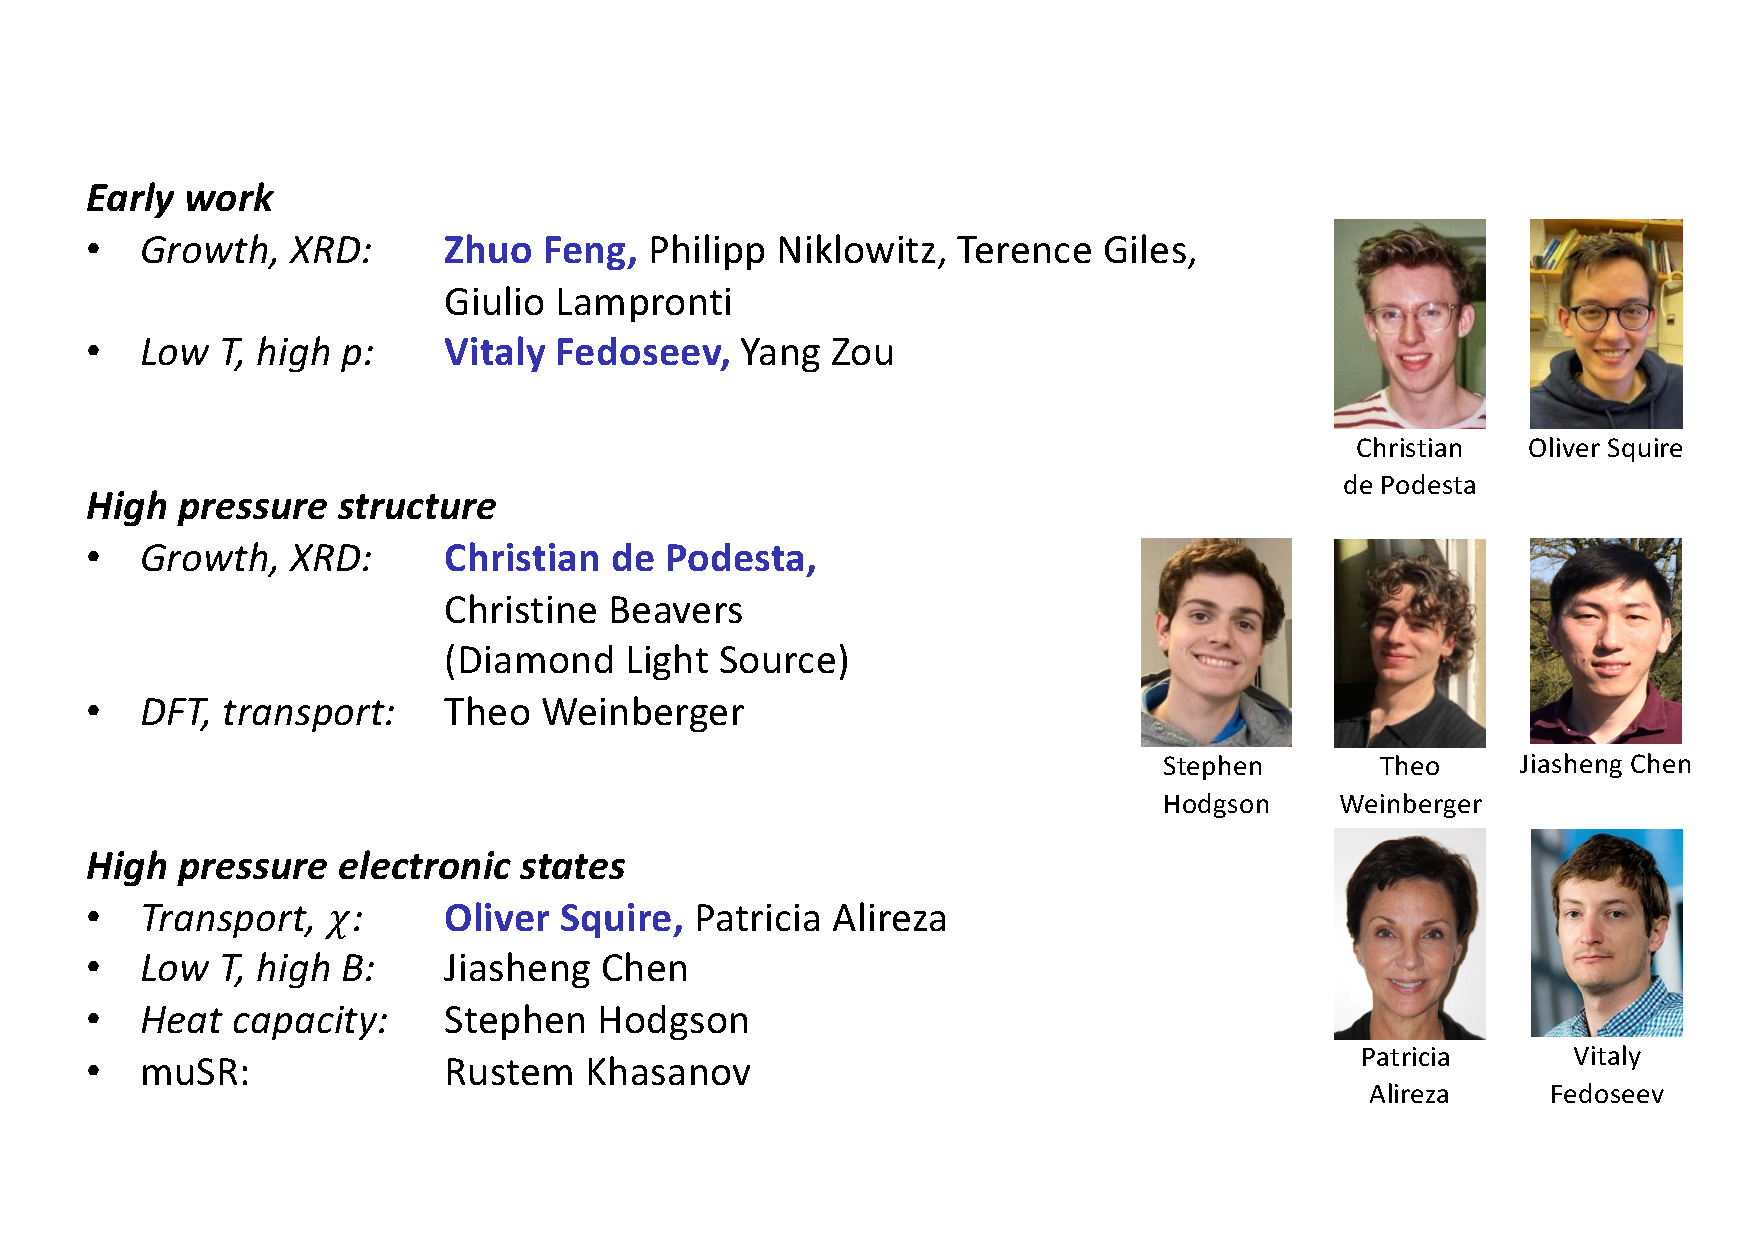
\includegraphics[width=1.25\textwidth]{GroupList}
\end{frame}

%%%%%%%%%%%%%%%%%%%%%%%%%%%%%%%%%%%%%%%%%%%%%%%%%%%%%%%%%%%%%%%%%%%%%%

\begin{frame}[plain,label=Conc]
\frametitle {Key contributors}
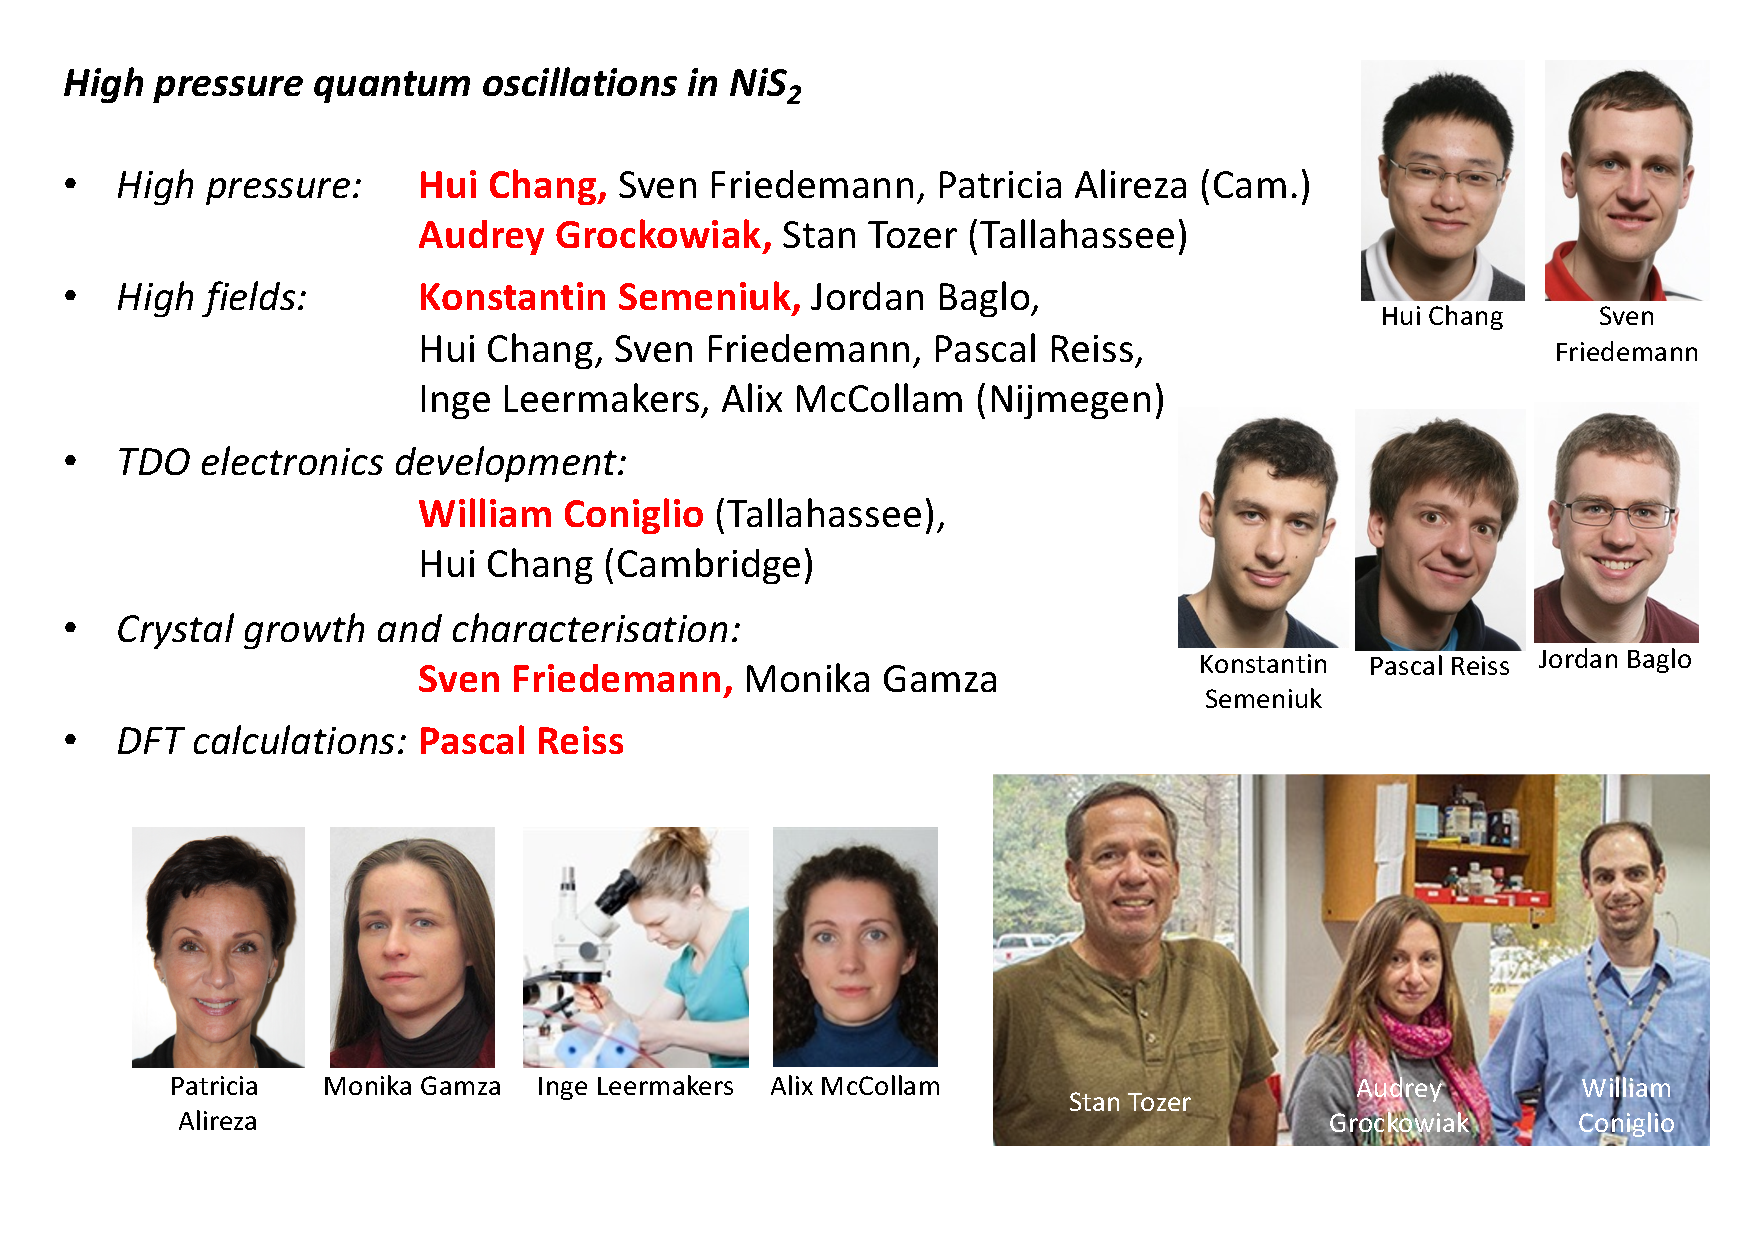
\includegraphics[width=1.25\textwidth]{GroupListNiS2}
%{\scriptsize
% \hl{YFe$_2$Ge$_2$}
% \begin{itemize}
% %\setlength{\baselineskip}{1.4em}
% \item{Samples:} \hfill
% \hl{Jiasheng Chen,} Zhuo Feng 
% %% \\ \raggedleft{Geetha Balakrishnan  (Warwick)}

% \item{Measurements:} \hfill  \hl{Konstantin Semeniuk,} Phil Brown %, Yang Zou, Peter Logg
% % \item{Low-$T$ magnetic susceptibility:} \hfill Christopher Harrison, \\
% %   \raggedleft{\hl{Philipp Niklowitz} (RHUL), Jordan Baglo}

% %\item{Band structure calculations:} \hfill {Pascal Reiss}
% \end{itemize}

% \hl{R$_3$T$_4$Sn$_{13}$}
% \begin{itemize}
% \setlength{\baselineskip}{1.4em}
% \item{Crystals:} \hfill
% J. Yang, B. Chen, \raggedleft{\hl{K. Yoshimura} (Kyoto and Hangzhou)}

% \item{High pressure:} \hfill
% \hl{Swee Goh,} Lina Klintberg
% \item{X-ray diffraction:} \hfill \hl{Paul Saines} 
% \end{itemize}

% \vspace{1em}


%  \hl{Bi-III}
% \begin{itemize}
% \item{Measurements:} \hfill 
% \hl {Phil Brown,} Konstantin Semeniuk, Alex Vasiljkovic

% \item{DFT calculations} \hfill
% \hl{Bartomeu Monserrat,} Chris Pickard, Diandian Wang
% \end{itemize}

% \vspace{1em}

% \hl{Fermi surface of pressure-metallised NiS$_2$}
% \begin{itemize}
% \item{Crystals:} \hfill \hl{Sven Friedemann,} Monika Gamza
% \item{High $p$ quantum oscillations:} \hfill \hl{Hui Chang, Sven Friedemann,} \\
% \raggedleft {Konstantin Semeniuk,} Jordan Baglo
% \item {High field measurements:} \hfill \hl{A. Grockowiak,} W. Coniglio, S. Tozer
%   (Tallahassee), \\ \raggedleft{I. Leermakers, A.
%   McCollam (Nijmegen)}

% \item{DFT calculations:} \hfill
% Pascal Reiss
%\end{itemize}

% \hl{NbFe$_2$}
% \begin{itemize}
% \setlength{\baselineskip}{1.4em}
% \item{Single crystals:} \hfill
% \hl{Will Duncan,} Andreas Neubauer,  \\ \raggedleft{Christian Pfleiderer
%   (RHUL, Munich)}


% % \item{$\mu$SR:} \hfill \hl{Daniela Rauch,} Stefan S\"ullow, \\
% % \raggedleft{M. Kraken, H. Luetkens, Jochen Litterst (Braunschweig)}

% % \item{ESR, dilatometry:} \hfill Thomas Bauer, \\ 
% % \raggedleft{Tobias F\"orster,  \hl{Manuel Brando} (Dresden)}

% \item{Magnetometry, resistivity:} \hfill
% \hl{Sven Friedemann,} Max Hirschberger
%   (Cambridge)

% \item{Neutron scattering:} \hfill
% \hl{Philipp Niklowitz,} Marijn Lucas (RHUL), Max Hirschberger, \\ 
% \raggedleft{Astrid
%   Schneidewind, Petr Cermak, Enrico Faulhaber (Munich)}
% \end{itemize}

% \hl{CeSb$_2$}
% \begin{itemize}
% \item{Crystals:} \hfill \hl{Zhuo Feng,} Takao
%   Ebihara (Shizuoka)

% \item{Measurements:} \hfill 
% \hl {Vitaly Fedoseev}, Yang Zou

% \item{High-$p$ x-rays:} \hfill
% \hl{Philipp Niklowitz,} Terence Giles, \raggedleft{Heribert Wilhelm}
% \end{itemize}

%\vspace{1em}


% \rule{\textwidth}{0.4pt}
% \begin{itemize}

% % \item{X-ray diffraction:} \hfill
% % Giulio Lampronti, Paul Saines 

% \item{High pressure training and support:} \hfill
% Patricia Alireza

% \item{Discussions, motivation and ideas:} \hfill
% \hl{Gil Lonzarich} % \\ \raggedleft{Philipp Niklowitz (RHUL)}

% \end{itemize}

%}

% \item{Discussions, motivation and ideas:} \hfill
% \hl{Gil Lonzarich,} \\ \raggedleft{Christoph Geibel, Manuel Brando, Sven Friedemann}

% \item{Neutron scattering:} \hfill
% \hl{Philipp Niklowitz (RHUL),} \\ 
% \raggedleft{Max Hirschberger, Astrid
%   Schneidewind, Enrico Faulhaber (Munich)}
%\end{itemize}


% \item{SQUID anvil cells, mini-coils:} \hfill
% \hl{Patricia Alireza}



% \item{High field measurements:} \hfill
% Mike Sutherland
%
%\begin{textblock}{4}(4, -5.2)
%\visible<2->{
%\begin{beamercolorbox}{postit}
%\begin{center}
%\textcolor{red}{Probably won't \\ get this far...}
%\end{center}
%\end{beamercolorbox}
%}
%\end{textblock}

\end{frame}







%%% Local Variables: 
%%% mode: latex
%%% TeX-master: "GroTalk.ho"
%%% End: 

%%%%%%%%%%%%%%%%%%%%%%%%%%%%%%%%%%%%%%%%%%%%%%%%%%%%%%%%%%%%%%%%%%%%%%%
%\section{Quantum Matter Gruppe}
%%%%%%%%%%%%%%%%%%%%%%%%%%%%%%%%%%%%%%%%%%%%%%%%%%%%%%%%%%%%%%%%%%%%%%

\begin{frame}[plain,label=Group]
\frametitle {Cambridge Quantum Matter Gruppe}
\centerline{\hspace{5em}\includegraphics[width=1.2\columnwidth]{\Figures/photos/Group/QM/GroupPicture2015.pdf}}
%\centerline{\hspace{5em}\small + 16 new PhD students since 2013}
\end{frame}

%%%%%%%%%%%%%%%%%%%%%%%%%%%%%%%%%%%%%%%%%%%%%%%%%%%%%%%%%%%%%%%%%%%%%%
%\section{Research Highlights}
%%%%%%%%%%%%%%%%%%%%%%%%%%%%%%%%%%%%%%%%%%%%%%%%%%%%%%%%%%%%%%%%%%%%%%
\begin{frame}[label=ResearchHighlights]
  %\frametitle{Forschungsthemen der Quantum Matter Gruppe}
\centerline{\includegraphics[width=1\textwidth]{\Figures/GroupAdvertising/ResearchHighlights}}
\becbox{1}{178 publications since 2011,\\ 8 Nature group, 15
  APL, 14 PRL, 1 PNAS}
\encbox

%\centerline{Approaching \pounds 5 Mio. external support since 2008}

\end{frame}

%%%%%%%%%%%%%%%%%%%%%%%%%%%%%%%%%%%%%%%%%%%%%%%%%%%%%%%%%%%%%%%%%%%%%%
\begin{frame}[label=ResearchSuccess]
%  \frametitle{Measures of success}
\hl{Recent fellowships}
\begin{small}
\begin{itemize}
\addtolength{\itemsep}{-0.3\baselineskip}
\item Stephen Rowley -- JRF Emmanuel College
\item Robert Smith -- JRF St. Catherine's College
\item Suchitra Sebastian -- JRF Trinity College, URF, King's Fellow
\item Swee Goh -- JRF Trinity College
\item Lina Klintberg -- JRF Newnham College
\item Sven Friedemann -- Feodor Lynen Fellow, Marie Curie Fellow
\item Sian Dutton -- Winton Fellow
\item Emma Pugh -- URF and Girton Fellow
\item Michael Sutherland -- URF, Corpus Christi Fellow
\end{itemize}
\end{small}

% \hl{186 publications} since 2008, \hl{3800 citations}
% \begin{small}
% \begin{itemize}
% \addtolength{\itemsep}{-0.3\baselineskip}
% \item
% 16 Applied Physics Letters
% \item
% 3 Nature and 8 Nature group
% \item
% 11 Physical Review Letters
% \item
% 2 Proceedings of the National Academy of Science
% \end{itemize}
% \end{small}


\hl{>100 invited plenary talks} since 2008
\begin{small}
\begin{itemize}
\addtolength{\itemsep}{-0.3\baselineskip}
\item
Gil Lonzarich: IOP Guthrie Medal and Royal Society Rumford Medal
\item
James Scott: MRS gold Medal
\item
Montu Saxena: IUPAP Young Scientist Medal, Presidential Medals Kaz. and Uzb.
\item 
Suchitra Sebastian: IUPAP Young Scientist Medal, IOP Moseley Medal
\end{itemize}
\end{small}
\end{frame}

%%% Local Variables: 
%%% mode: latex
%%% TeX-master: "GroTalk"
%%% End: 

%

%%%%%%%%%%%%%%%%%%%%%%%%%%%%%%%%%%%%%%%%%%%%%%%%%%%%%%%%%%%%%%%%%%%%%%
% \section{Quantum criticality -- more info}
% \subsection{Relaxation rates}
%%%%%%%%%%%%%%%%%%%%%%%%%%%%%%%%%%%%%%%%%%%%%%%%%%%%%%%%%%%%%%%%%%%%%%
\begin{frame}[label=quancrit1]
\frametitle{Quantum criticality-1}

\begin{columns}[t]
\column{0.6\textwidth}
\centerline{~}

Fluctuating \hl{local order parameter} $m(\vec r, \vec t)$, response
function (susceptibility)
\[ \chi_{\vec q \omega} = \chi_{\vec q} \frac{1}{1-i\omega/\Gamma_\vec q} \]

\begin{itemize}
\item Relaxation rate $\Gamma_\vec q \sim {\chi_\vec q}^{-1}$
\item $\Gamma_\vec q \rightarrow 0$ at $T_N$, $\bf q=\vec Q$
\end{itemize}

\column{0.4\textwidth}
\centerline{~}
\includegraphics[width=\columnwidth,clip=on]{\Figures/QuanCrit/GammaQ-0}
\end{columns}

\vspace{4ex}
\centerline{\hl{Power spectrum} of $m$:
$\langle |m_{\vec q\omega}|^2 \rangle = \left(n_\omega + \frac{1}{2}\right) \Im(\chi_{\vec q \omega})$}

\end{frame}


%%%%%%%%%%%%%%%%%%%%%%%%%%%%%%%%%%%%%%%%%%%%%%%%%%%%%%%%%%%%%%%%%%%%%%
% \subsection{Thermal excitation}
%%%%%%%%%%%%%%%%%%%%%%%%%%%%%%%%%%%%%%%%%%%%%%%%%%%%%%%%%%%%%%%%%%%%%%
\begin{frame}[label=quancrit2]{Quantum criticality-2}

\begin{columns}[t]
  \column{0.6\textwidth}
  \centerline{~}
  \[ \chi_{\vec q \omega} = \chi_{\vec q} \frac{1}{1-i\omega/\Gamma_\vec q} \]

  \[ \langle |m_{\vec q\omega}|^2 \rangle = \left(n_\omega + \frac{1}{2}\right) \Im(\chi_{\vec q \omega}) \]

\begin{itemize}
\item<2->
  Integrals over $\vec q$ and $\omega$, e.g.
\end{itemize}

  \column{0.4\textwidth}
  \centerline{~}
  \multiinclude[<visible@+- | +->][graphics={width=\columnwidth,clip=on},format=pdf]{\Figures/QuanCrit/GammaQ}

\end{columns}
\visible<2->{\[ \langle m(\vec r) m(0) \rangle \propto \int{d^3 \vec q \chi_\vec q e^{-i \vec q \vec r}} \int {d\omega \left(n_\omega + \frac {1}{2}\right) \frac{\omega/\Gamma_\vec q}{1+\omega^2/\Gamma_\vec q^2}} \]

\raggedleft{(Bose-factor $n_\omega \rightarrow \frac{k_B T}{\hbar\omega}$ if $k_B
T >> \hbar \omega$)}}

\begin{itemize}
\item<3->
  \hl{Classical} critical behaviour: $k_B T >> \hbar \Gamma_\vec q$ for
  critical modes $\vec q$.  Integrals separable, frequency integral
  gives $k_B T$ (\hl{equipartition}). Only static susc.  $\chi_\vec q$
  survives.  

\item<4->
  \hl{Quantum critical} behaviour: $k_B T$ falls inside dispersion
  $\Gamma_\vec q$.  Dynamics (via $\Gamma_\vec q$) influence result.
\end{itemize}

\end{frame}



%%% Local Variables: 
%%% mode: latex
%%% TeX-master: "GroTalk"
%%% End: 

%%%%%%%%%%%%%%%%%%%%%%%%%%%%%%%%%%%%%%%%%%%%%%%%%%%%%%%%%%%%%%%%%%%%%%
%\section{Novel electronic states}

%%%%%%%%%%%%%%%%%%%%%%%%%%%%%%%%%%%%%%%%%%%%%%%%%%%%%%%%%%%%%%%%%%%%%
\subsection{Tunability of correlated electron systems}
%%%%%%%%%%%%%%%%%%%%%%%%%%%%%%%%%%%%%%%%%%%%%%%%%%%%%%%%%%%%%%%%%%%%%%
\begin{frame}[label=ElecLiquid]
\frametitle{Tunability of correlated systems}

\centerline{\multiinclude[<visible@+-| +->][format=pdf,graphics={width=0.9\columnwidth}]{\Figures/FreeElec/ElecLiquid}}
\vspace{2ex}

\visible<3-> {\centerline{\parbox{0.9\columnwidth}{High quality crystals
      $\rightarrow$ tune to border of low temperature order
      $\rightarrow$ anomalous metallic state or new ordered phase.}}}


\end{frame}

%%%%%%%%%%%%%%%%%%%%%%%%%%%%%%%%%%%%%%%%%%%%%%%%%%%%%%%%%%%%%%%%%%%%%%
%\subsection{Superconductivity and magnetism}
%%%%%%%%%%%%%%%%%%%%%%%%%%%%%%%%%%%%%%%%%%%%%%%%%%%%%%%%%%%%%%%%%%%%%%

% %%%%%%%%%%%%%%%%%%%%%%%%%%%%%%%%%%%%%%%%%%%%%%%%%%%%%%%%%%%%%%%%%%%%%%
% \subsection{CePd$_2$Si$_2$}
%%%%%%%%%%%%%%%%%%%%%%%%%%%%%%%%%%%%%%%%%%%%%%%%%%%%%%%%%%%%%%%%%%%%%%
\begin{frame}[label=CPS]
\frametitle{CePd$_2$Si$_2$: heavy-fermion magnet to unconventional superconductor}
\begin{columns}[t]
  \column{0.37\textwidth}
  \begin{itemize}
  \item<1-> Antiferro\-magnet below $T_N\simeq 10 ~\mathrm K$.

  \item<1-> $T_N$ depends on pressure.

  \item<1->  Magnetism suppressed near 2.8 GPa.

  \item<1-> Anomalous resistivity $T$-dependence.
  \end{itemize}

\vspace{1em}
\centerline{\scriptsize [Mathur {\em et al.}, Nature {\bf 394,} (1998) 39]}
  \column{0.63\textwidth}
\vspace{0em}
  \centerline{\multiinclude[<visible@1-|1->][graphics={width=0.95\columnwidth},format=pdf]{\Figures/cps/cpsphasesnormal}}
 
\end{columns}
%\onslide+<1->
\begin{center}
\hl{Superconductivity and anomalous normal state.}
\end{center}
\end{frame}


%%%%%%%%%%%%%%%%%%%%%%%%%%%%%%%%%%%%%%%%%%%%%%%%%%%%%%%%%%%%%%%%%%%%%%
\begin{frame}[label=ThreshMagn]
\frametitle{Magnetic interaction model}

\centerline{\includegraphics[width=\textwidth]{\Figures/CritConcepts/MagnInter2}}

\end{frame}



%%%%%%%%%%%%%%%%%%%%%%%%%%%%%%%%%%%%%%%%%%%%%%%%%%%%%%%%%%%%%%%%%%%%%%
\begin{frame}[label=CPS]
\frametitle{From narrow band, $f$-electron, low-$T_c$ to
  $d$-electron high-$T_c$}
\centerline{\includegraphics[width=0.9\textwidth]{\Figures/Phasedias/CePd2Si2/cpsbfaComparison}}

\begin{columns}[t]
\column{0.5\textwidth}
\centerline{\scriptsize \hspace{5em} [Mathur {\em et al.}, Nature {\bf 394,} 39  (1998)]}

\column{0.5\textwidth}
\centerline{\scriptsize [from Hashimoto Science {\bf 336,} 1554 (2012)]}
\end{columns}
\end{frame}

%%%%%%%%%%%%%%%%%%%%%%%%%%%%%%%%%%%%%%%%%%%%%%%%%%%%%%%%%%%%%%%%%%%%%%
\begin{frame}[label=phasedias]
%\frametitle{Phase diagrams in correlated quantum systems}
%\frametitle{Examine Fermi surface evolution near quantum phase transitions}
%\vspace{-3ex}
\centerline{%
\includegraphics[width=\columnwidth,clip=on]{\Figures/Phasedias/phasedias10}}
\end{frame}



%%%%%%%%%%%%%%%%%%%%%%%%%%%%%%%%%%%%%%%%%%%%%%%%%%%%%%%%%%%%%%%%%%%%%
\subsection{Material space}
%%%%%%%%%%%%%%%%%%%%%%%%%%%%%%%%%%%%%%%%%%%%%%%%%%%%%%%%%%%%%%%%%%%%%

\begin{frame}[label=Diversity]

\frametitle{Plenty of room in material space}
\only<beamer>{%
\only<1>{%
\vspace{2em}
\centerline{\includegraphics[angle=90,width=0.9\columnwidth]{\Figures/Diversity/PerSysen.jpg}}
}
}
\pause                          
%\centerline{\multiinclude[<visible@1->][graphics={width=0.9\columnwidth},format=pdf]{\Figures/Diversity/Diversity}}
\centerline{\multiinclude[<visible@+-| +->][graphics={width=0.9\columnwidth},format=pdf]{\Figures/Diversity/Diversity}}

\end{frame}



% %%%%%%%%%%%%%%%%%%%%%%%%%%%%%%%%%%%%%%%%%%%%%%%%%%%%%%%%%%%%%%%%%%%%%%
% \begin{frame}[label=Funding]
% \frametitle{Networks, fellowships and funding}

% \begin{itemize}
% \item \hl{International networks}: ICAM, 
% \begin{itemize}
% \item
% ICAM

% \end{frame}

% %%%%%%%%%%%%%%%%%%%%%%%%%%%%%%%%%%%%%%%%%%%%%%%%%%%%%%%%%%%%%%%%%%%%%%
% \subsection{Fermi surface instabilities}
% %%%%%%%%%%%%%%%%%%%%%%%%%%%%%%%%%%%%%%%%%%%%%%%%%%%%%%%%%%%%%%%%%%%%%%
% \begin{frame}[label=FermiSurface]
%   \frametitle{Fermi surface: surface in momentum space on which low energy excitations are possible}
% \only<1>{
% \vspace{5em}
% \centerline{\includegraphics[width=\columnwidth]{\Figures/Lectures/ElecGas/FermiSea.jpg}}
% %\centerline{\small A. Schofield (1998)}
% }

% \begin{columns}[t]
% \column{0.5\textwidth}
% \visible<2->{
% \centerline{\includegraphics[height=0.98\columnwidth]{\Figures/FreeElec/copper.jpg}}
% \centerline{Copper}}

% \column{0.5\textwidth}
% \visible<3->{
% \centerline{\includegraphics[height=0.98\columnwidth]{\Figures/NbFe2Overview/band84}}
% \centerline{NbFe$_2$}}
% \end{columns}

% \end{frame}







%%% Local Variables: 
%%% mode: latex
%%% TeX-master: "GroTalk"
%%% End: 



%%%%%%%%%%%%%%%%%%%%%%%%%%%%%%%%%%%%%%%%%%%%%%%%%%%%%%%%%%%%%%%%%%%%%
\savegeometry{beamergeo}
\begin{emptyframe}
    \frametitle{Truncated mass divergence in the Mott metal NiS$_2$}
    \centerline{ \includegraphics[width=0.95\columnwidth]{\data/NiS2/FiguresNiS2/NiS2Summary.pdf}}
\vspace{-1 em}
\vfill
\centerline{\makebox[\linewidth]{\rule{0.85\textwidth}{0.4pt}}}
\centerline{\scriptsize Semeniuk {\it et al.} PNAS e2301456120 (2023)}
\end{emptyframe}
\loadgeometry{beamergeo}

%%%%%%%%%%%%%%%%%%%%%%%%%%%%%%%%%%%%%%%%%%%%%%%%%%%%%%%%%%%%%%%%%%%%%
\savegeometry{beamergeo}
\begin{emptyframe}
    \frametitle{Superconductivity in the Hund's metals (Y/Lu)Fe$_2$Ge$_2$}
    \centerline{ \includegraphics[width=0.85\columnwidth]{\data/YFe2Ge2/FiguresYFG/Overview/YFe2Ge2Summary.pdf}}
\vspace{-1 em}
\vfill 
\centerline{\makebox[\linewidth]{\rule{0.85\textwidth}{0.4pt}}}
\centerline{\scriptsize Chen {\it et al.} PRL {\bf 125,} 237002 (2020), Baglo {\it et al.} PRL {\bf 129,} 046402 (2022)}
\end{emptyframe}
\loadgeometry{beamergeo}

%%%%%%%%%%%%%%%%%%%%%%%%%%%%%%%%%%%%%%%%%%%%%%%%%%%%%%%%%%%%%%%%%%%%%
\savegeometry{beamergeo}
\begin{emptyframe}
    \frametitle{Quantum oscillations in the new superconductor UTe$_2$}
    \centerline{ \includegraphics[width=0.75\columnwidth]{\data/UTe2/FiguresUTe2/Overview/SummaryUTe2-2.png}}
\vspace{-1 em}
\vfill 
\centerline{\makebox[\linewidth]{\rule{0.85\textwidth}{0.4pt}}}
\centerline{\scriptsize Eaton Nature Comm., arXiv:2302.04758 (2023), Wu arXiv:2305.19033 (2023), Weinberger arXiv:2307.00568 (2023)}
\end{emptyframe}
\loadgeometry{beamergeo}



%%%%%%%%%%%%%%%%%%%%%%%%%%%%%%%%%%%%%%%%%%%%%%%%%%%%%%%%%%%%%%%%%%%%%
\savegeometry{beamergeo}
\begin{emptyframe}
%\begin{frame}[plain,label=TitlePage]
\begin{center}
\textcolor{Blue}{Electronic and structural instabilities} \\
\vspace{0.5em}
{\footnotesize F. M. Grosche} \\
{\footnotesize \em Cavendish Laboratory, Cambridge} \\
\vspace{0.1em}
\end{center}
\vspace{0.0em}
%\centerline{\multiinclude[<visible@+-| +->][format=pdf,graphics={width=\columnwidth}]{\Figures/FermInstab/QPTScenariosHostGuest2}}
\setbeamercovered{invisible}
\begin{tikzpicture}
    \node[anchor=south west,inner sep=0] (image) at (0,0) {
        \centerline{ \includegraphics[width=\columnwidth]{IntroPicture1}}
    };
    \pause
    \begin{scope}[x={(image.south east)},y={(image.north west)}]
        \draw[Blue,line width=1 mm] (0, 1)--(1, 0);
        \draw[Blue,line width=1 mm] (0, 0)--(1, 1);
    \end{scope}
\end{tikzpicture}

\begin{itemize}
    \item<1-> Projects in Quantum Matter group, happy to discuss
    \item<2-> Focus instead on CeSb$_2$, new high pressure superconductor
    \item<3-> And on anomalous low-$T$ resistivity in quasiperiodic systems
\end{itemize}
\setbeamercovered{transparent}
\end{emptyframe}
\loadgeometry{beamergeo}



%%% Local Variables: 
%%% mode: latex
%%% TeX-master: "GroTalk.ho"
%%% End: 

%%%%%%%%%%%%%%%%%%%%%%%%%%%%%%%%%%%%%%%%%%%%%%%%%%%%%%%%%%%%%%%%%%%%%%
\savegeometry{beamergeo}
\begin{emptyframe}
    \frametitle{Truncated mass divergence in the Mott metal NiS$_2$}
    \centerline{ \includegraphics[width=0.95\columnwidth]{\data/NiS2/FiguresNiS2/NiS2Summary.pdf}}
\vspace{-1 em}
\vfill
\centerline{\makebox[\linewidth]{\rule{0.85\textwidth}{0.4pt}}}
\centerline{\scriptsize Semeniuk {\it et al.} PNAS e2301456120 (2023)}
\end{emptyframe}
\loadgeometry{beamergeo}

%%%%%%%%%%%%%%%%%%%%%%%%%%%%%%%%%%%%%%%%%%%%%%%%%%%%%%%%%%%%%%%%%%%%%
\savegeometry{beamergeo}
\begin{emptyframe}
    \frametitle{Superconductivity in the Hund's metals (Y/Lu)Fe$_2$Ge$_2$}
    \centerline{ \includegraphics[width=0.85\columnwidth]{\data/YFe2Ge2/FiguresYFG/Overview/YFe2Ge2Summary.pdf}}
\vspace{-1 em}
\vfill 
\centerline{\makebox[\linewidth]{\rule{0.85\textwidth}{0.4pt}}}
\centerline{\scriptsize Chen {\it et al.} PRL {\bf 125,} 237002 (2020), Baglo {\it et al.} PRL {\bf 129,} 046402 (2022)}
\end{emptyframe}
\loadgeometry{beamergeo}

%%%%%%%%%%%%%%%%%%%%%%%%%%%%%%%%%%%%%%%%%%%%%%%%%%%%%%%%%%%%%%%%%%%%%
\savegeometry{beamergeo}
\begin{emptyframe}
    \frametitle{Quantum oscillations in the new superconductor UTe$_2$}
    \centerline{ \includegraphics[width=0.75\columnwidth]{\data/UTe2/FiguresUTe2/Overview/SummaryUTe2-2.png}}
\vspace{-1 em}
\vfill 
\centerline{\makebox[\linewidth]{\rule{0.85\textwidth}{0.4pt}}}
\centerline{\scriptsize Eaton Nature Comm., arXiv:2302.04758 (2023), Wu arXiv:2305.19033 (2023), Weinberger arXiv:2307.00568 (2023)}
\end{emptyframe}
\loadgeometry{beamergeo}



<<<<<<< HEAD
\section{High-$p$ QO}


%%%%%%%%%%%%%%%%%%%%%%%%%%%%%%%%%%%%%%%%%%%%%%%%%%%%%%%%%%%%%%%%%%%%%%

\begin{frame}[plain,label=Conc2]
\frametitle {Mass renormalisation on the threshold of Mott localisation}
\includegraphics[width=1.2\textwidth]{\data/NiS2/FiguresNiS2/CollaboratorsNiS2/CollaboratorsNiS2.pdf}
\end{frame}

%%%%%%%%%%%%%%%%%%%%%%%%%%%%%%%%%%%%%%%%%%%%%%%%%%%%%%%%%%%%%%%%%%%%%%
\subsection{Mott Isolator NiS$_2$}
%%%%%%%%%%%%%%%%%%%%%%%%%%%%%%%%%%%%%%%%%%%%%%%%%%%%%%%%%%%%%%%%%%%%%%
\begin{frame}[label=NiS2-1]
\frametitle{Charge transfer Mott insulator Ni(S/Se)$_2$}
\begin{columns}[t]
\column{0.5\textwidth}
\centerline{~}
\centerline{\includegraphics[width=0.8\columnwidth]{\Figures/Structures/NiS2/NiS2.png}}

\begin{itemize}

\item
Descended from NiO
\item
fcc lattice of Ni in $d^8$ configuration.
\item
Charge gap between $3d$ UHB and S/Se $p$ states. 

\end{itemize}
\column{0.5\textwidth}
\centerline{~}
\centerline{\includegraphics[width=\columnwidth]{\data/NiS2/FiguresNiS2/BackgroundInfo/NiS2MiyasakaAnn}}
\end{columns}
\vspace{0.5em}
\centerline{Tuneable by isoelectronic Se doping or by pressure.}
\vspace*{\fill}
\vspace{-0.25em}
%\vspace{3.5em}
\centerline{\makebox[\linewidth]{\rule{0.85\textwidth}{0.4pt}}}
\centerline{\scriptsize Miyasaka et al, JPSJ {\bf 69,} 3166 (2000)}
\end{frame}





%%%%%%%%%%%%%%%%%%%%%%%%%%%%%%%%%%%%%%%%%%%%%%%%%%%%%%%%%%%%%%%%%%%%%%
\subsection{High pressure NiS$_2$}
%%%%%%%%%%%%%%%%%%%%%%%%%%%%%%%%%%%%%%%%%%%%%%%%%%%%%%%%%%%%%%%%%%%%%%
\begin{frame}[label=NiS2-1]
\frametitle{Pressure induced Mott metal-insulator transition in NiS$_2$}
%\centerline{\includegraphics[width=\columnwidth]{\Figures/NiS2/PhaseDiaNiS2.pdf}}
\centerline{\includegraphics[width=0.8\columnwidth]{\data/NiS2/FiguresNiS2/Resistivity/SvenRes}}
\begin{itemize}
\item
Resistivity, liquid pressure medium, patterned anvils.

\item
Metallisation above 3 GPa in flux-grown high quality samples,
$\rho_0 < 1~\mu \Omega \mathrm {cm}$.

\item 
Search for quantum oscillations.

% \item
% AFM qcp at 8 GPa.
\end{itemize}
\vspace*{\fill}
\vspace{-0.25em}
%\vspace{3.5em}
\centerline{\makebox[\linewidth]{\rule{0.85\textwidth}{0.4pt}}}
\centerline{\scriptsize S. Friedemann Sci. Rep. {\bf 6,} 2535 (2016)}
\end{frame}

%%%%%%%%%%%%%%%%%%%%%%%%%%%%%%%%%%%%%%%%%%%%%%%%%%%%%%%%%%%%%%%%%%%%%
\subsection{High pressure QO}
%%%%%%%%%%%%%%%%%%%%%%%%%%%%%%%%%%%%%%%%%%%%%%%%%%%%%%%%%%%%%%%%%%%%%%
\begin{frame}[label=QuantOsc]
\frametitle{Quantum oscillations}
%\frametitle{Quantenoszillationen}

\visible<1->{\centerline{\includegraphics[width=0.8\columnwidth]{\Figures/Lectures/QuantOsc/Sr2RuO4Osc}}}


\visible<2->{
\centerline{\includegraphics[width=0.9\textwidth]{\Figures/FermInstab/QuantOsc-Xray.pdf}}}

\end{frame}

%%%%%%%%%%%%%%%%%%%%%%%%%%%%%%%%%%%%%%%%%%%%%%%%%%%%%%%%%%%%%%%%%%%%%%
%\subsection{rf methods}
%%%%%%%%%%%%%%%%%%%%%%%%%%%%%%%%%%%%%%%%%%%%%%%%%%%%%%%%%%%%%%%%%%%%%%
%%%%%%%%%%%%%%%%%%%%%%%%%%%%%%%%%%%%%%%%%%%%%%%%%%%%%%%%%%%%%%%%%%%%%%
\begin{frame}[label=DACcoil]
\frametitle{Quantum oscillation measurements at high pressure}

\centerline{\includegraphics[width=0.9\columnwidth]{\Figures/Pressure/TDO/QO-DAC-TDO}}
\begin{itemize}

\item
%Developed for magnetic susceptibility measurements, 
Coil in sample space, filling factor $\sim 0.3$

\item
At high frequency, probe metallic skin depth $s \propto
\sqrt{\rho/\omega}$.

\item 
Skin depth $\rightarrow$ excluded sample volume $\rightarrow$ \\ \raggedleft{coil
self-inductance $\rightarrow$ resonance frequency.}
% Resolution $\delta L/L \simeq f \frac{s}{r} \delta \rho/\rho$.\\ {\small ($f =$ coil filling factor, $r = $ sample radius)} 
\end{itemize}


\vspace*{\fill}
%\vspace{3.5em}
\centerline{\makebox[\linewidth]{\rule{0.85\textwidth}{0.4pt}}}
\centerline{\scriptsize Alireza, Rev. Sci. Inst. {\bf 74,} 4728 (2003)}

\end{frame}


%%%%%%%%%%%%%%%%%%%%%%%%%%%%%%%%%%%%%%%%%%%%%%%%%%%%%%%%%%%%%%%%%%%%%
\subsection{NiS$_2$ Quantum oscillations}
%%%%%%%%%%%%%%%%%%%%%%%%%%%%%%%%%%%%%%%%%%%%%%%%%%%%%%%%%%%%%%%%%%%%%
\begin{frame}[label=NiS2Mass]
  \frametitle{Fermi surface and effective mass in pressure metallised NiS$_2$}
\centerline{\includegraphics[width=\columnwidth]{\data/NiS2/FiguresNiS2/HomeDetail/QOPlot3FigText}}
%
%\begin{itemize}
%\item Amplitude boosted compared to lower pressure measurement.
%\item 6 kT frequency $\rightarrow$ large hole pocket as in DFT calculation. 
%
%\item Mass $\simeq 5\times$ band mass.
%%\item Amplitude much higher than at lower $p$ near Mott transition:
% %  phase coexistence at low $p$?
%\end{itemize}


\vspace*{\fill}
\centerline{\makebox[\linewidth]{\rule{0.85\textwidth}{0.4pt}}}
\begin{center}
{\scriptsize K. Semeniuk, H. Chang, J. Baglo, S. Friedemann, A. Grockowiak, \\
A. McCollam et al (Nijmegen/Tallahassee/Cambridge),  \hlb{PNAS e2301456120 (2023)}}
\end{center}

\end{frame}





%%%%%%%%%%%%%%%%%%%%%%%%%%%%%%%%%%%%%%%%%%%%%%%%%%%%%%%%%%%%%%%%%%%%%
\subsection{Mass and frequency vs. $p$}
% %%%%%%%%%%%%%%%%%%%%%%%%%%%%%%%%%%%%%%%%%%%%%%%%%%%%%%%%%%%%%%%%%%%%%
\begin{frame}[label=QONiS2]
\frametitle{Evolution of Fermi surface and effective mass in NiS$_2$}
\vspace{0.5em}

\centerline{\includegraphics[width=0.9\columnwidth]{\data/NiS2/FiguresNiS2/PressureDependence/Fig3_PressureDep4FignoLabels}}
\begin{itemize}
\item
Fermi surface stays large on approaching Mott transition, but
effective mass rises.
\item
Divergence \hl{inside} insulating region.
\end{itemize}

\vspace*{\fill}
\centerline{\makebox[\linewidth]{\rule{0.85\textwidth}{0.4pt}}}
\begin{center}
{\scriptsize K. Semeniuk, H. Chang, J. Baglo, S. Friedemann, A. Grockowiak, \\
A. McCollam et al (Nijmegen/Tallahassee/Cambridge),  \hlb{PNAS e2301456120 (2023)}}
\end{center}

\end{frame}


%%%%%%%%%%%%%%%%%%%%%%%%%%%%%%%%%%%%%%%%%%%%%%%%%%%%%%%%%%%%%%%%%%%%%
%\subsection{Quantum oscillations in NiS$_2$}
% %%%%%%%%%%%%%%%%%%%%%%%%%%%%%%%%%%%%%%%%%%%%%%%%%%%%%%%%%%%%%%%%%%%%%
\begin{frame}[label=QONiS2-2]
  \frametitle{Truncated mass divergence in Mott metal NiS$_2$}
  
  \centerline{\includegraphics[width=0.9\columnwidth]{\data/NiS2/FiguresNiS2/PhaseDiaOverview/Fig1_PhaseDiaWideFig}}
  %\centerline{\includegraphics[width=0.8\columnwidth]{\data/NiS2/FiguresNiS2/}}
  \begin{itemize}
  \item<1->
  {Inverse mass extrapolates to zero on insulating side.}
  % \item
  % Mott transition first order even for $T\rightarrow 0$?
  \item<visible@2->
  {Divergence inaccessible (first order transition, DMFT).}
  
  \end{itemize}
  
  \vspace*{\fill}
  \vspace{-0.25em}
  %\vspace{3.5em}
  \centerline{\makebox[\linewidth]{\rule{0.85\textwidth}{0.4pt}}}
  %\centerline{\scriptsize K. Semeniuk, J. Baglo, A. Grockowiak,
  %  S. Tozer, NHMFL 2017}
  \centerline{\scriptsize Georges, Kotliar, Krauth, Rozenberg
    Rev. Mod. Phys. {\bf 68,} 13 (1996)}
  \end{frame}
  
  


<<<<<<< HEAD
=======
\section{Host-guest structures}
=======
\section{Structural quantum critical point}
%%%%%%%%%%%%%%%%%%%%%%%%%%%%%%%%%%%%%%%%%%%%%%%%%%%%%%%%%%%%%%%%%%%%%%

%\subsection{(Sr/Ca)$_3$Ir$_4$Sn$_{13}$}
%\section{Structure}

% %%%%%%%%%%%%%%%%%%%%%%%%%%%%%%%%%%%%%%%%%%%%%%%%%%%%%%%%%%%%%%%%%%%%%%
% \begin{frame}[label=CIS-1]
% \frametitle{Quasiskutterudite material family R$_3$T$_4$X$_{13}$}
% \begin{columns}[t]
% \column{0.5\textwidth}
% \begin{itemize}
% % \item
% % R = earth alkaline or rare earth, T = transition metal, X = group-4 (Ge, Sn).
% \item
% Combination of filled skutterudite (LaRu$_4$P$_{12}$) and A15 structure (Nb$_3$Sn): (X'R$_3$) T$_4$X$_{12}$. 
% \item
% Two structure types, both cubic: phase $I$ and $I'$. In $I'$ the lattice constant is doubled: superlattice distortion on $I$. 
% \item
% Here, investigate Sr$_3$Ir$_4$Sn$_{13}$ and substitution series to  Ca$_3$Ir$_4$Sn$_{13}$.

% \item
% Transition $I \rightarrow I'$ on cooling, superlattice formation.
% \end{itemize}
% {\small \centerline{[Klintberg PRL (2012)]}}
% \column{0.5\textwidth}
% \centerline{~}
% \centerline {\includegraphics[width=\columnwidth]{\Figures/R3T4X13/Superlattice_QCP_resub_Figure1}}
% \end{columns}
% \end{frame}

%%%%%%%%%%%%%%%%%%%%%%%%%%%%%%%%%%%%%%%%%%%%%%%%%%%%%%%%%%%%%%%%%%%%%%
\begin{frame}[plain,label=Conc]
\frametitle {Soft phonons at structural qcp and in quasiperiodic materials}
\includegraphics[width=1.2\textwidth]{\data/R3Ir4Sn13/Collaborators/CollabCISblue}
\end{frame}


%%%%%%%%%%%%%%%%%%%%%%%%%%%%%%%%%%%%%%%%%%%%%%%%%%%%%%%%%%%%%%%%%%%%%%
\subsection{Structural transition in R$_3$T$_4$Sn$_{13}$}
%%%%%%%%%%%%%%%%%%%%%%%%%%%%%%%%%%%%%%%%%%%%%%%%%%%%%%%%%%%%%%%%%%%%%%
\begin{frame}[label=CIS-1]
\frametitle{Cubic quasi-skutterudites R$_3$T$_4$Sn$_{13}$}
%\frametitle{(Sr/Ca)$_3$Ir$_4$Sn$_{13}$}

\centerline{\includegraphics[width=0.8\columnwidth]{\Figures/R3T4X13/Sr3Ir4Sn13_amb-Struct3}}
\begin{itemize}
\item
Second-order lattice instability at $T^* \simeq 147~\rm K$ in
Sr$_3$Ir$_4$Sn$_{13}$, superconductivity at $T_c \simeq 5~\rm K$.
%\item
% Investigate Sr$_3$Ir$_4$Sn$_{13}$ and substitution series to  Ca$_3$Ir$_4$Sn$_{13}$.

\end{itemize}
\vspace*{\fill}
%\vspace{3.5em}
\centerline{\makebox[\linewidth]{\rule{0.85\textwidth}{0.4pt}}}
\centerline{\scriptsize L. Klintberg, S. Goh et al. PRL  {\bf 109,} 237008 (2012)}
\end{frame}




%%%%%%%%%%%%%%%%%%%%%%%%%%%%%%%%%%%%%%%%%%%%%%%%%%%%%%%%%%%%%%%%%%%%%%
\subsection{Structural qcp, $\rho \propto T$}
%%%%%%%%%%%%%%%%%%%%%%%%%%%%%%%%%%%%%%%%%%%%%%%%%%%%%%%%%%%%%%%%%%%%%%
\begin{frame}[label=CIS-2]
\frametitle{Superlattice transition and superconductivity are tuned by
  composition and pressure in (Sr/Ca)$_3$Ir$_4$Sn$_{13}$}
\begin{columns}[t]
\column{0.5\textwidth}
\vspace{-1.25em}
\centerline{~}
%\vspace{2em}
\centerline{\includegraphics[height=0.96\columnwidth]{\Figures/R3T4X13/Superlattice_QCP_resub_Figure2-annot}}
\column{0.5\textwidth}
\centerline{~}
\visible<2->{\centerline {\includegraphics[height=0.98\columnwidth]{\Figures/R3T4X13/CISRTnoInsetLabel}}}
\end{columns}

\begin{itemize}
\item
\visible<1->{Structural transition $T^*$ reduced by Ca-substitution
  and pressure.}
\item
\visible<2->{$T_c$ rises on approaching critical pressure.}
\item
\visible<3->{\hl {$T$-linear
  resistivity at $p_c$.}}
\end{itemize}

\vspace*{\fill}
%\vspace{3.5em}
\centerline{\makebox[\linewidth]{\rule{0.85\textwidth}{0.4pt}}}
\centerline{\scriptsize L. Klintberg, S. Goh et al. PRL  {\bf 109,} 237008 (2012)}
\end{frame}

%%%%%%%%%%%%%%%%%%%%%%%%%%%%%%%%%%%%%%%%%%%%%%%%%%%%%%%%%%%%%%%%%%%%%%
%\subsection{Phonon softening}
\begin{frame}[label=CIS-phonons]
\frametitle{Role of phonon dispersion near critical pressure in (Sr/Ca)$_3$Ir$_4$Sn$_{13}$}
\centerline{\includegraphics[width=0.8\columnwidth]{\Figures/R3T4X13/Phonons}}
\begin{itemize}
\item
Optical mode associated with superlattice transition goes soft near
$p_c$.

% \item
% Dispersion presumably linear, but entire, narrow-width branch is
% lowered.

\item
Can cause linear $\rho(T)$ for $k_B T>\hbar \Omega$ (frequency scale
of soft branch), as
\end{itemize}
\begin{align*} \Delta\rho_{ph}(T) \propto \sum_{\bf q} \alpha_{(tr) \bf q}^2 &T (\partial  \underuparrow{n_{\bf q}}/\partial T )_{\omega_{\bf q}} \rightarrow  T \sum
  \omega_{\bf q}^{-1} (\propto T \lambda ) \\
&{\scriptstyle \left(e^{\hbar \omega /k_B T} - 1\right)^{-1}  }
\end{align*}



\end{frame}





%%% Local Variables: 
%%% mode: latex
%%% TeX-master: "GroTalk"
%%% End: 

\section{Quasiperiodic structures}
>>>>>>> fa24158 (Wed morning Shanghai talk)
\begin{frame}[plain,label=Conc]
  \frametitle {Soft phonons at structural qcp and in quasiperiodic materials}
  \includegraphics[width=1.2\textwidth]{\data/R3Ir4Sn13/Collaborators/CollabCISblue}
\end{frame}  

%%%%%%%%%%%%%%%%%%%%%%%%%%%%%%%%%%%%%%%%%%%%%%%%%%%%%%%%%%%%%%%%%%%%%%
\subsection{High pressure structures}
%%%%%%%%%%%%%%%%%%%%%%%%%%%%%%%%%%%%%%%%%%%%%%%%%%%%%%%%%%%%%%%%%%%%%%
\begin{frame}[label=BiRes]
\frametitle{High pressure phases of Bismuth}
%\vspace{-3em}
\centerline{\multiinclude[<+- | visible@+>] [graphics={width=0.9\columnwidth},format=pdf]{\Figures/Bi/Bi3/BiOverviewLog}}

%\vspace{-2em}
\begin{itemize}
\item <visible@1-> Semimetal with $\sim 1$ e$^-$ per $10^5$ atoms at
  low pressure.

\item <visible@2-> Carrier concentration drops with increasing pressure.

\item <visible@6-> Bi-II, III: high carrier concentration, superconductivity.

% \item <visible@6-> High carrier concentration in high-pressure structure.
\end{itemize}

\vspace*{\fill}
\centerline{\makebox[\linewidth]{\rule{0.85\textwidth}{0.4pt}}}
\centerline{\scriptsize P. Brown Physics Procedia {\bf 75,} 29 (2015), Li PRB {\bf 95,} 024510  (2017)}
\end{frame}

%%%%%%%%%%%%%%%%%%%%%%%%%%%%%%%%%%%%%%%%%%%%%%%%%%%%%%%%%%%%%%%%%%%%%%
\subsection{$\rho \propto T$, quasiperiodic structure}
%%%%%%%%%%%%%%%%%%%%%%%%%%%%%%%%%%%%%%%%%%%%%%%%%%%%%%%%%%%%%%%%%%%%%%

\begin{frame}[label=BiSuper1]
\frametitle{Superconductivity and $T$-linear resistivity in high pressure Bi-III}
\centerline{\multiinclude[<+- | visible@+>] [graphics={width=0.95\columnwidth},format=pdf]{\Figures/Bi/Bi3/BiRes1Figure}}
%\centerline{\scriptsize poster by Phil Brown, \hl{P6.3 on Thursday afternoon}}

\begin{itemize}
\item $T_c \simeq 7.2 ~ \text{K}$, linear $\rho(T)$ at low $T$.
% \item Upper critical field $B_{c2}\simeq 2~\text{T}$, suggesting
% type-II.
\item Compare to Pb, neighbour in periodic table, $T_c \simeq 7.2~\text{K}$.
\item<visible@2-> Incommensurate host-guest structure of Bi-III.

\end{itemize}

% \vspace*{\fill}
% %\vspace{0.5em}
% \centerline{\makebox[\linewidth]{\rule{0.85\textwidth}{0.4pt}}}
% \centerline{\scriptsize also Li PRB {\bf 95,} 024510  (2017)}
\vspace*{\fill}
\centerline{\makebox[\linewidth]{\rule{0.85\textwidth}{0.4pt}}}
\centerline{\hlb{\scriptsize P. Brown Sci. Adv. {\bf 4:}eaao4793 (2018)}}
\end{frame}

%%%%%%%%%%%%%%%%%%%%%%%%%%%%%%%%%%%%%%%%%%%%%%%%%%%%%%%%%%%%%%%%%%%%%%
\subsection{Sliding mode}
%%%%%%%%%%%%%%%%%%%%%%%%%%%%%%%%%%%%%%%%%%%%%%%%%%%%%%%%%%%%%%%%%%%%%%
\begin{frame}[label=BiIntro]
\frametitle{Bi-III phase: host-guest structure}
\centerline{\includegraphics[width=0.85\columnwidth]{\Figures/Structures/Bismuth/Bi3Struct}}

\visible<2->{

\centerline{\includegraphics[width=\columnwidth]{\Figures/Bi/PhasonModecrop}}
}

\begin{itemize}
\item <visible@2->Phason is like fourth acoustic mode (but damped).

\end{itemize}

\vspace*{\fill}
\vspace{1.5em}
\centerline{\makebox[\linewidth]{\rule{0.85\textwidth}{0.4pt}}}
\centerline{\scriptsize McMahon, Degtyareva, Nelmes PRL {\bf 85}, 4896
  (2000), Reed and Ackland, PRL {\bf 84,} 5580 (2000)}
\end{frame}


%%%%%%%%%%%%%%%%%%%%%%%%%%%%%%%%%%%%%%%%%%%%%%%%%%%%%%%%%%%%%%%%%%%%%%
%\subsection{Phonon dispersion}
%%%%%%%%%%%%%%%%%%%%%%%%%%%%%%%%%%%%%%%%%%%%%%%%%%%%%%%%%%%%%%%%%%%%%%
\begin{frame}
\frametitle{Bi-III phason branch: flat and soft}
\centerline{\includegraphics[width=0.7\textwidth]{\Figures/Bi/Bi3/Phonons/Monserrat0217/PhononDispersionFigure}}
\begin{itemize}
\item
Low-lying phason modes (2 chains per unit cell) in
42-atom approximant
\item
Little dispersion perpendicular to $c$-axis. % , monatomic-chain dispersion
% parallel $c$.
\item
1D dispersion $\rightarrow$ large contribution to e$^-$-phonon $\lambda$.
\end{itemize}

\end{frame}



%%%%%%%%%%%%%%%%%%%%%%%%%%%%%%%%%%%%%%%%%%%%%%%%%%%%%%%%%%%%%%%%%%%%%%
\subsection{Role of approximants}
%%%%%%%%%%%%%%%%%%%%%%%%%%%%%%%%%%%%%%%%%%%%%%%%%%%%%%%%%%%%%%%%%%%%%%
\begin{frame}
\frametitle{Role of approximants, demonstrated in potassium}

\centerline{\includegraphics[width=0.9\textwidth]{\data/K/PhononCalc/Approximants}}

\begin{itemize}
\item
Low-lying phason (sliding) modes in large approximants.
\end{itemize}

\vspace*{\fill}
\centerline{\makebox[\linewidth]{\rule{0.85\textwidth}{0.4pt}}}
\centerline{\scriptsize K. Atalar to be published (2023)}

\end{frame}

%%%%%%%%%%%%%%%%%%%%%%%%%%%%%%%%%%%%%%%%%%%%%%%%%%%%%%%%%%%%%%%%%%%%%%
\begin{frame}
\frametitle{e-ph coupling in potassium approximants}

\centerline{\includegraphics[width=0.9\textwidth]{\data/K/PhononCalc/Lambda}}

\begin{itemize}
\item
Obtain $\lambda$ directly from the calculated phonon spectrum.
\item
Soft modes in large approximants produce $\lambda > 2$.

\end{itemize}

\vspace*{\fill}

\centerline{\makebox[\linewidth]{\rule{0.85\textwidth}{0.4pt}}}
\centerline{\scriptsize K. Atalar to be published (2023)}

\end{frame}



%%% Local Variables: 
%%% mode: latex
%%% TeX-master: "GroTalk.tex"
%%% End: 

<<<<<<< HEAD
>>>>>>> 9a4db31 (iterate Wed morning)

\section{YFe$_2$Ge$_2$}
%%%%%%%%%%%%%%%%%%%%%%%%%%%%%%%%%%%%%%%%%%%%%%%%%%%%%%%%%%%%%%%%%%%%%%

\begin{frame}[plain,label=YFGCollab]
\frametitle {Mass renormalisation in the Hund's metal YFe$_2$Ge$_2$}
\vspace{1em}
\includegraphics[width=\textwidth]{\data/yfe2ge2/FiguresYFG/Collaborators/GroupListYFG}
%\vspace*{\fill}
%\vspace{0.5em}
%%\centerline{\makebox[\linewidth]{\rule{0.85\textwidth}{0.4pt}}}
%\begin{center}
%{\scriptsize [ Baglo PRL {\bf 129,} 046402 (2022)]}
%  \end{center}
\end{frame}

%%%%%%%%%%%%%%%%%%%%%%%%%%%%%%%%%%%%%%%%%%%%%%%%%%%%%%%%%%%%%%%%%%%%%%
\subsection{YFe$_2$Ge$_2$}
%%%%%%%%%%%%%%%%%%%%%%%%%%%%%%%%%%%%%%%%%%%%%%%%%%%%%%%%%%%%%%%%%%%%%%
\begin{frame}[label=YFGIntro]
\frametitle{Superconductivity and anomalous normal state in YFe$_2$Ge$_2$}
%\frametitle{Quantenoszillationen}

\centerline{\includegraphics[width=\textwidth]{\data/yfe2ge2/FiguresYFG/GrowthHorizontalFlux2019/Transition} }
\begin{itemize}
\item
Iron-based superconductor with a group-4 element
\item
Comparatively 3D Fermi surface structure 
\item
High Sommerfeld coefficient, $C/T \simeq \SI{100}{\mJ/(\mol\kelvin^2)}$
\end{itemize}
\centerline{\hl{Origin of high $C/T$?}}

\vspace*{\fill}
%\vspace{3.5em}
\centerline{\makebox[\linewidth]{\rule{0.85\textwidth}{0.4pt}}}
\begin{center}
{\scriptsize [Zou Phys Status Solidi (RRL) {\bf 8,} 928
  (2014); Chen PRL {\bf 116,} 127001 (2016), Chen PRB {\bf 99,} 020501 (R) (2019), Chen PRL {\bf 125,} 237002 (2020), \hlb{Baglo PRL {\bf 129,} 046402 (2022)}]}
  \end{center}
\end{frame}





%%%%%%%%%%%%%%%%%%%%%%%%%%%%%%%%%%%%%%%%%%%%%%%%%%%%%%%%%%%%%%%%%%%%%%
\begin{frame}[plain,label=YFGFermiSurface]
\frametitle{DFT Fermi surface in YFe$_2$Ge$_2$}
\includegraphics[width=1.2\textwidth]{\data/yfe2ge2/FiguresYFG/BandStruct/Wien2kSummary.pdf}
\end{frame}

%%%%%%%%%%%%%%%%%%%%%%%%%%%%%%%%%%%%%%%%%%%%%%%%%%%%%%%%%%%%%%%%%%%%%%
\subsection{QO results}
%%%%%%%%%%%%%%%%%%%%%%%%%%%%%%%%%%%%%%%%%%%%%%%%%%%%%%%%%%%%%%%%%%%%%%%
%\begin{frame}[label=QuantOsc]
%\frametitle{Quantum oscillations}
%%\frametitle{Quantenoszillationen}
%
%\visible<1->{\centerline{\includegraphics[width=0.8\columnwidth]{\Figures/Lectures/QuantOsc/Sr2RuO4Osc}}}
%
%
%\visible<2->{
%\centerline{\includegraphics[width=0.9\textwidth]{\Figures/FermInstab/QuantOsc-Xray.pdf}}}
%
%\end{frame}


%%%%%%%%%%%%%%%%%%%%%%%%%%%%%%%%%%%%%%%%%%%%%%%%%%%%%%%%%%%%%%%%%%%%%%
\begin{frame}[plain,label=YFGQO]
\frametitle{Quantum oscillations in YFe$_2$Ge$_2$}
\includegraphics[width=1.2\textwidth]{\data/yfe2ge2/FiguresYFG/QO/QOPlotFig.pdf}

\begin{itemize}
\item Cambridge 20.4 Tesla cryomagnet (Julian/Lonzarich)
\item de Haas-van Alphen study in mutual inductance setup
\item Rotator with three sample stages
\end{itemize}
\end{frame}

%%%%%%%%%%%%%%%%%%%%%%%%%%%%%%%%%%%%%%%%%%%%%%%%%%%%%%%%%%%%%%%%%%%%%%
\begin{frame}[plain,label=YFGRot]
\frametitle{Resolving the Fermi surface in YFe$_2$Ge$_2$}
\includegraphics[width=1.2\textwidth]{\data/yfe2ge2/FiguresYFG/QO/Waterfall_cFig}

\vspace{2em}
\centerline{Track signatures of three pockets with angle against $c$-axis}
%\vspace*{\fill}
%\vspace{3.5em}
%\centerline{\makebox[\linewidth]{\rule{0.85\textwidth}{0.4pt}}}
%\begin{center}
%{\scriptsize [Baglo arXiv 2104.11791 (2021)]}
%  \end{center}
\end{frame}

%%%%%%%%%%%%%%%%%%%%%%%%%%%%%%%%%%%%%%%%%%%%%%%%%%%%%%%%%%%%%%%%%%%%%%
\subsection{Fermiology in YFe$_2$Ge$_2$}
%%%%%%%%%%%%%%%%%%%%%%%%%%%%%%%%%%%%%%%%%%%%%%%%%%%%%%%%%%%%%%%%%%%%%%
\begin{frame}[plain,label=YFGOverviewFS]
\frametitle{Fermi surface and carrier masses in YFe$_2$Ge$_2$}
%\frametitle{Electron counting in YFe$_2$Ge$_2$}
\includegraphics[width=1.2\textwidth]{\data/yfe2ge2/FiguresYFG/QO/MassStudyComments}

\visible<2->{
\mbox{Masses \hl{uniformly} renormalised $\rightarrow$ 
 \hl{local} mechanism causes narrow bands.}
}

\end{frame}






%%% Local Variables: 
%%% mode: latex
%%% TeX-master: "GroTalk.ho"
%%% End: 


\section{LuFe$_2$Ge$_2$}
%%%%%%%%%%%%%%%%%%%%%%%%%%%%%%%%%%%%%%%%%%%%%%%%%%%%%%%%%%%%%%%%%%%%%%
\begin{frame}[label=YFGIntro2b]

\frametitle{Magnetic quantum phase transition in (Lu/Y)Fe$_2$Ge$_2$}
\centerline{\includegraphics[width=0.9\columnwidth]{\data/yfe2ge2/FiguresYFG/PhaseDiaAnnotPerSys2.pdf}}
\begin{itemize}
\item 
LuFe$_2$Ge$_2$ magnetic order: FM planes, stacked antiferromagnetically
%\item
%$V_0 ($YFe$_2$Ge$_2) = 164.8 \Ang^3$, $V_0 ($LuFe$_2$Ge$_2) =
%159.3 \Ang^3$ 
%
%\hfill $\implies \Delta V_0/V_0 \simeq 3.5 \%$
%(corresponds to about 4 GPa).
%%\item Require around 3 GPa to tune YFe$_2$Ge$_2$ to qcp.
\end{itemize}
\end{frame}

%%%%%%%%%%%%%%%%%%%%%%%%%%%%%%%%%%%%%%%%%%%%%%%%%%%%%%%%%%%%%%%%%%%%%%
\subsection{Crystal growth}
%%%%%%%%%%%%%%%%%%%%%%%%%%%%%%%%%%%%%%%%%%%%%%%%%%%%%%%%%%%%%%%%%%%%%%
\begin{frame}[label=LFGGrowth]
\frametitle{LuFe$_2$Ge$_2$ high quality crystal growth using liquid transport method}
\centerline{\includegraphics[width=\columnwidth]{\data/LuFe2Ge2/FiguresLFG/CrystalGrowth/LiquidTransportLFG2}}

\begin{center}
Liquid transport (horizontal flux) method boosts ratio flux/solute \\
and reduces precipitation temperature.
\end{center}
\vspace*{\fill}
%\vspace{3.5em}
\centerline{\makebox[\linewidth]{\rule{0.85\textwidth}{0.4pt}}}
\centerline{\scriptsize Chen PRL {\bf 125,} 237002 (2020)}
\end{frame}



%%%%%%%%%%%%%%%%%%%%%%%%%%%%%%%%%%%%%%%%%%%%%%%%%%%%%%%%%%%%%%%%%%%%%%
\subsection{SDW + superconductivity}
%%%%%%%%%%%%%%%%%%%%%%%%%%%%%%%%%%%%%%%%%%%%%%%%%%%%%%%%%%%%%%%%%%%%%%
\begin{frame}[label=LFGAnomalies]
\frametitle{Magnetism and superconductivity in LuFe$_2$Ge$_2$}
\centerline{\multiinclude[<+-|visible@+>][format=pdf,graphics={width=0.9\textwidth}]{\data/LuFe2Ge2/FiguresLFG/SDW/Transitions}}

\begin{itemize}
\item <1-> In clean crystals: sharp SDW transition at $T_N \simeq \SI{7}{\kelvin}$.
\item <2-> Superconductivity at $T_c \simeq \SI{0.8}{\kelvin}$.
\end{itemize}
\end{frame}

%%%%%%%%%%%%%%%%%%%%%%%%%%%%%%%%%%%%%%%%%%%%%%%%%%%%%%%%%%%%%%%%%%%%%%
\subsection{QCP}
%%%%%%%%%%%%%%%%%%%%%%%%%%%%%%%%%%%%%%%%%%%%%%%%%%%%%%%%%%%%%%%%%%%%%%
\begin{frame}[label=QCP]
\frametitle{Is there a quantum critical point in LuFe$_2$Ge$_2$?}
\centerline{\includegraphics[width=\textwidth]{\data/LuFe2Ge2/FiguresLFG/SDW/qcp}}

\begin{itemize}
\item
Single crystals from (Y/Lu)Fe$_2$Ge$_2$ substitution series
\item
$\chi$ shows strongest $T$-dependence where $T_N \rightarrow 0$.
\item
Much weaker $T$-dependence at other compositions suggests low-$T$ tail in $\chi$ is intrinsic, not caused by magnetic impurities.
\end{itemize}
\end{frame}


%%%%%%%%%%%%%%%%%%%%%%%%%%%%%%%%%%%%%%%%%%%%%%%%%%%%%%%%%%%%%%%%%%%%%%
\subsection{Superconductivity}
%%%%%%%%%%%%%%%%%%%%%%%%%%%%%%%%%%%%%%%%%%%%%%%%%%%%%%%%%%%%%%%%%%%%%%
\begin{frame}[label=LFGSupercon]
\frametitle{Evidence for superconductivity in LuFe$_2$Ge$_2$}
\centerline{\includegraphics[width=\textwidth]{\data/LuFe2Ge2/FiguresLFG/Supercon/Superconductivity1}}

In clean crystals:
\begin{columns}[t]
\column{0.5\textwidth}
\begin{itemize}
\item Resistive transition $T_c \simeq \SI{0.8}{\kelvin}$
\item Tiny heat capacity signature
\end{itemize}
\column{0.5\textwidth}
\begin{itemize}
\item DC magnetisation weak
\item $B_{c2}'/T_c$ same as in YFe$_2$Ge$_2$
\end{itemize}
\end{columns}

\begin{center}
{Small superconducting fraction similar to early YFe$_2$Ge$_2$.} \\
\end{center}

$B_{c2} \simeq \SI{0.43}{\tesla} \implies \xi \simeq \SI{280}{\angstrom}$ twice that of YFe$_2$Ge$_2$ \\
\raggedleft $\rightarrow$ need longer mean free path. 
\end{frame}




% 
%%%%%%%%%%%%%%%%%%%%%%%%%%%%%%%%%%%%%%%%%%%%%%%%%%%%%%%%%%%%%%%%%%%%%%%
%\subsection{New superconductors}
%%%%%%%%%%%%%%%%%%%%%%%%%%%%%%%%%%%%%%%%%%%%%%%%%%%%%%%%%%%%%%%%%%%%%%%
%\begin{frame}[label=LaH10]
%\frametitle{Record $T_c$ in high-pressure LaH$_{10}$}
%\centerline{\includegraphics[width=\textwidth]{\Figures/Phasedias/UnconvSupercon/LaH10}}
%%\vspace{0em}
%
%\begin{center}
%$T_c$ extends up to \SI{283}{\kelvin}, {\bf maybe much higher}
%
%\end{center}
%\small{
%\begin{itemize}
%%Success of computationally assisted materials discovery.
%\item
%Can LaH$_{10}$-style superconductivity extend to ambient pressure?
%\item
%Probably not; such high phonon frequencies require compression.
%\item
%\textcolor{red}{Need alternative pairing interaction with high energy scale:} \\
%\textcolor{red}{\bf magnetic interaction in metals reaches
%  up to 3,000 K.}
%\end{itemize}}
%\end{frame}
%
%%%%%%%%%%%%%%%%%%%%
\begin{frame}[label=KFA-YFG-Motivation]
\frametitle{From KFe$_2$As$_2$ to YFe$_2$Ge$_2$}
\centerline{\includegraphics[width=\textwidth]{\data/yfe2ge2/FiguresYFG/Overview/KFA-YFG-Motivation-crop}}

\vspace{2em}

\begin{itemize}
\item
Search for analogues to Fe-As superconductors.

\item
KFe$_2$As$_2$ ($T_c \simeq 3.8 ~\text{K}$): high $C/T \simeq 100
~\text{mJ/mol K}^{2}$.

\item
YFe$_2$Ge$_2$ has similarly high $C/T$, apparently same Fe oxidation
number as in
KFe$_2$As$_2$.
\end{itemize}
\centerline{\hl{Origin of high $C/T$?}}
%\centerline{among the highest in transition metal compounds?}

\vspace*{\fill}
% \vspace{1.5em}
\centerline{\makebox[\linewidth]{\rule{0.85\textwidth}{0.4pt}}}
\centerline{\scriptsize Reid Supercond. Sci. Technol. {\bf 25,} 084013 (2012), Avila JMMM {\bf 270,} 51 (2004)}
\end{frame}


%%%%%%%%%%%%%%%%%%%%%%%%%%%%%%%%%%%%%%%%%%%%%%%%%%%%%%%%%%%%%%%%%%%%%%
\subsection{The route to YFe$_2$Ge$_2$}
%%%%%%%%%%%%%%%%%%%%%%%%%%%%%%%%%%%%%%%%%%%%%%%%%%%%%%%%%%%%%%%%%%%%%%
\begin{frame}[label=YFGIntro1]
\frametitle{From narrow-band, $f$-electron low-$T_c$ to $d$-electron high-$T_c$}
\centerline{\includegraphics[width=\columnwidth]{\Figures/PhaseDias/CePd2Si2/cpsbfaComparison}}

\vspace{1em}
\centerline{We need more unconventional superconductors!}

\vspace*{\fill}
%\vspace{3.5em}
\centerline{\makebox[\linewidth]{\rule{0.85\textwidth}{0.4pt}}}
\centerline{\scriptsize Mathur Nature {\bf 394,} 39 (1998), Hashimoto
  Science {\bf 336,} 1554 (2012)}
\end{frame}



%%%%%%%%%%%%%%%%%%%%%%%%%%%%%%%%%%%%%%%%%%%%%%%%%%%%%%%%%%%%%%%%%%%%%%
\subsection{The (Lu/Y)Fe$_2$Ge$_2$ system}
%%%%%%%%%%%%%%%%%%%%%%%%%%%%%%%%%%%%%%%%%%%%%%%%%%%%%%%%%%%%%%%%%%%%%%
\begin{frame}[label=EarlyWork]
\frametitle{Early work on (Y/Lu)Fe$_2$Ge$_2$}
\centerline{\includegraphics[width=\textwidth]{\data/yfe2ge2/FiguresYFG/Overview/YFGEarlyWork}}
\begin{itemize} %\itemsep 8pt
\item
Antiferromagnetic transition in LuFe$_2$Ge$_2$ near 10 K.

% Unusually high $\gamma = C/T$ of about 100 mJ/mol K$^2$.
% \item
% $V_0 ($YFe$_2$Ge$_2) = 164.8 \Ang^3$, $V_0 ($LuFe$_2$Ge$_2) =
% 159.3 \Ang^3$ 

% \hfill $\implies \Delta V_0/V_0 \simeq 3.5 \%$
% (corresponds to about 4 GPa).
%\item Require around 3 GPa to tune YFe$_2$Ge$_2$ to qcp.

\item
Magnetic susceptibility $\chi_{SI} \sim 10^{-3}$. \\ Moderately enhanced Wilson ratio $R_W \simeq 2.5$.

% \item
% Fe oxidation state appears same as in KFe$_2$As$_2$ ($+2.5$).

\end{itemize}
\end{frame}

%%%%%%%%%%%%%%%%%%%%%%%%%%%%%%%%%%%%%%%%%%%%%%%%%%%%%%%%%%%%%%%%%%%%%%


%%%%%%%%%%%%%%%%%%%%%%%%%%%%%%%%%%%%%%%%%%%%%%%%%%%%%%%%%%%%%%%%%%%%%
\begin{frame}[label=YFGIntro2]
  \frametitle{Magnetism and enhanced $C/T$ in  (Lu/Y)Fe$_2$Ge$_2$}
  \centerline{\includegraphics[width=\columnwidth]{\data/yfe2ge2/FiguresYFG/YFGLFGCompare-crop.pdf}}
  \begin{itemize} %\itemsep 8pt
  \item LuFe$_2$Ge$_2$ transition at $T_N \sim \SI{10}{\kelvin}$, YFe$_2$Ge$_2$ no magnetic order
  \item
  Unusually high $\gamma = C/T$ of about 100 mJ/mol K$^2$.
  \item
  $V_0 ($YFe$_2$Ge$_2) = 164.8 \Ang^3$, $V_0 ($LuFe$_2$Ge$_2) =
  159.3 \Ang^3$ 
  
  \hfill $\implies \Delta V_0/V_0 \simeq 3.5 \%$
  (corresponds to about 4 GPa).
  %\item Require around 3 GPa to tune YFe$_2$Ge$_2$ to qcp.
  
  \item
  Magnetic susceptibility $\chi_{SI} \sim 10^{-3}$. \\ Moderately enhanced Wilson ratio $R_W \simeq 2.5$.
  
  %\item
  %Fe oxidation state appears same as in KFe$_2$As$_2$ ($+2.5$).
  
  \end{itemize}
  \end{frame}

%%%%%%%%%%%%%%%%%%%%%%%%%%%%%%%%%%%%%%%%%%%%%%%%%%%%%%%%%%%%%%%%%%%%%%
\subsection{Neutrons}
%%%%%%%%%%%%%%%%%%%%%%%%%%%%%%%%%%%%%%%%%%%%%%%%%%%%%%%%%%%%%%%%%%%%%%
\begin{frame}[label=YFGNeutrons]
\frametitle{Neutron scattering in YFe$_2$Ge$_2$}
\centerline{\includegraphics[width=\columnwidth]{\data/yfe2ge2/FiguresYFG/Neutrons/Wo19}}

\end{frame}



%%%%%%%%%%%%%%%%%%%%%%%%%%%%%%%%%%%%%%%%%%%%%%%%%%%%%%%%%%%%%%%%%%%%%%
\subsection{First-generation samples}
%%%%%%%%%%%%%%%%%%%%%%%%%%%%%%%%%%%%%%%%%%%%%%%%%%%%%%%%%%%%%%%%%%%%%%
\begin{frame}[label=YFGFirstGen]
\frametitle{Superconductivity in YFe$_2$Ge$_2$, first-generation samples}
\centerline{\includegraphics[width=\columnwidth]{\data/yfe2ge2/FiguresYFG/SampleSummaries/FirstGenSamples/FirstGenSamplesSummary}}
\begin{itemize}
\item
Polycrystals (induction-furnace) or single crystals (flux).
\item
Resistance ratios $< 60$. 
\item
Resistive transitions but no heat capacity anomaly at $T_c$.
\end{itemize}

\vspace*{\fill}
% \vspace{1.5em}
\centerline{\makebox[\linewidth]{\rule{0.85\textwidth}{0.4pt}}}
\centerline{\scriptsize [Zou Phys Status Solidi (RRL) {\bf 8,} 928
  (2014); Kim Phil. Mag. {\bf 95,} 804 (2015)]}
\end{frame}


%%%%%%%%%%%%%%%%%%%%%%%%%%%%%%%%%%%%%%%%%%%%%%%%%%%%%%%%%%%%%%%%%%%%%%
\subsection{Growth studies}
%%%%%%%%%%%%%%%%%%%%%%%%%%%%%%%%%%%%%%%%%%%%%%%%%%%%%%%%%%%%%%%%%%%%%%
\begin{frame}[label=YFGSecondGen]
\frametitle{Growth improvements lead to bulk superconductivity in polycrystals}
\centerline{\includegraphics[width=\columnwidth]{\data/yfe2ge2/FiguresYFG/SampleSummaries/SecondGenSamples/SecondGenSamplesOverview}}


\end{frame}

%%%%%%%%%%%%%%%%%%%%%%%%%%%%%%%%%%%%%%%%%%%%%%%%%%%%%%%%%%%%%%%%%%%%%%
\begin{frame}[label=YFGSecondGen]
\frametitle{Growth study in YFe$_2$Ge$_2$ polycrystals}
% \framezoom<1><2>(0cm,0cm)(2cm,1.5cm)
% \framezoom<1><3>(1cm,3cm)(2cm,1.5cm)
% \framezoom<1><4>(3cm,2cm)(3cm,2cm)
%\TPGrid{10}{10}
\centerline{\includegraphics[width=\columnwidth]{\data/yfe2ge2/FiguresYFG/SampleSummaries/SecondGenSamples/GrowthStudyResults.png}}
\begin{textblock}{4}[0.5, 0.5](7, -6.5)
\visible<2->{
\begin{beamercolorbox}{postit}
\begin{center}
\textcolor{red}{\small Fe-rich melt\\
ensures full \\occupation of Fe-site}
\end{center}
\end{beamercolorbox}
}
\end{textblock}
\end{frame}




%%%%%%%%%%%%%%%%%%%%%%%%%%%%%%%%%%%%%%%%%%%%%%%%%%%%%%%%%%%%%%%%%%%%%%
\subsection{High purity YFe$_2$Ge$_2$}
%%%%%%%%%%%%%%%%%%%%%%%%%%%%%%%%%%%%%%%%%%%%%%%%%%%%%%%%%%%%%%%%%%%%%%
\begin{frame}[label=YFGThirdGen]
\frametitle{Towards high quality single crystals of YFe$_2$Ge$_2$}

\begin{columns}[T]
\column{0.7\textwidth}
\begin{itemize}
\item
{\small Sn flux growth from high quality polycrystals (grown from Fe-rich melt).

\item
Experimenting with temperature profiles, crucible orientation, growth protocol has gradually produced \hl{RRR $\mathbf{\sim 500}$.}

\item
Sharp bulk transitions. Resistivity still $T^{3/2}$. }
\end{itemize}

\column{0.3\textwidth}
\centerline{\includegraphics[width=\columnwidth]{\data/yfe2ge2/FiguresYFG/SampleSummaries/GrowthSpring19/SamplesPhoto}}
\end{columns}

\vspace{1em}
{\includegraphics[width=1.02\columnwidth]{\data/yfe2ge2/FiguresYFG/SampleSummaries/GrowthSpring19/HeatCapResistivity}}


\end{frame}

%%%%%%%%%%%%%%%%%%%%%%%%%%%%%%%%%%%%%%%%%%%%%%%%%%%%%%%%%%%%%%%%%%%%%%
\subsection{Crystal growth}
%%%%%%%%%%%%%%%%%%%%%%%%%%%%%%%%%%%%%%%%%%%%%%%%%%%%%%%%%%%%%%%%%%%%%%
\begin{frame}[plain,label=YFGBulkSupercon]
\frametitle{Bulk superconductivity in high quality single crystals of YFe$_2$Ge$_2$}
\includegraphics[width=1.2\textwidth]{\data/yfe2ge2/FiguresYFG/GrowthHorizontalFlux2019/BulkSupercon}
\end{frame}


%%%%%%%%%%%%%%%%%%%%%%%%%%%%%%%%%%%%%%%%%%%%%%%%%%%%%%%%%%%%%%%%%%%%%%
\subsection{Heat capacity}
%%%%%%%%%%%%%%%%%%%%%%%%%%%%%%%%%%%%%%%%%%%%%%%%%%%%%%%%%%%%%%%%%%%%%%
\begin{frame}[label=YFGHeatCapKFA]
\frametitle{Heat capacity to very low temperatures}

\centerline{\includegraphics[width=\columnwidth]{\data/yfe2ge2/FiguresYFG/HeatCap/Dresden0519/HCYFGKFACompare}}
\begin{itemize}
\item
Dilution fridge measurements confirm sharp bulk transition in new
generation of YFe$_2$Ge$_2$ single crystals.
\item
Upturn at low temperature (nuclear contribution) prevents definitive
conclusion about gap structure and residual $\gamma$.
\item
Similarity with KFe$_2$As$_2$. 
\end{itemize}

\end{frame}


%%%%%%%%%%%%%%%%%%%%%%%%%%%%%%%%%%%%%%%%%%%%%%%%%%%%%%%%%%%%%%%%%%%%%%
\subsection{muSR}
%%%%%%%%%%%%%%%%%%%%%%%%%%%%%%%%%%%%%%%%%%%%%%%%%%%%%%%%%%%%%%%%%%%%%%
\begin{frame}[label=YFGmuSRIntro]
\frametitle{Transverse field muSR measurements}
\[
A_{TF} = A_0 \exp(-(\sigma t)^2/2) \cos\left(\gamma \mu
  \langle  B\rangle t+\phi\right )
+ A_{bg} \cos\left(\gamma \mu B_{bg} t + \phi \right)
\]
\centerline{\includegraphics[width=0.9\columnwidth]{\data/yfe2ge2/FiguresYFG/muSR2019/muSRtDependence}}
\centerline{First attempt at ISIS with Pabitra Biswas and Adroja Devashibhai}
\end{frame}


%%%%%%%%%%%%%%%%%%%%%%%%%%%%%%%%%%%%%%%%%%%%%%%%%%%%%%%%%%%%%%%%%%%%%%
\begin{frame}[label=YFGmuSRSummary]
\frametitle{Transverse field muSR}

\centerline{\includegraphics[width=\columnwidth]{\data/yfe2ge2/FiguresYFG/muSR2019/muSRResultSummary}}
\end{frame}

%%%%%%%%%%%%%%%%%%%%%%%%%%%%%%%%%%%%%%%%%%%%%%%%%%%%%%%%%%%%%%%%%%%%%%
%\subsection{Comparison to KFe$_2$As$_2$}
\subsection{Fermi surface structure}
%\subsection{$c-$axis contraction}
%%%%%%%%%%%%%%%%%%%%%%%%%%%%%%%%%%%%%%%%%%%%%%%%%%%%%%%%%%%%%%%%%%%%%%
\begin{frame}[label=CollapsedTetragonala]
\frametitle{High pressure KFe$_2$As$_2$ similar to YFe$_2$Ge$_2$}

\centerline{\includegraphics[width=0.95\columnwidth]{\data/yfe2ge2/FiguresYFG/FermiSurface/CompareKFA-YFG4}}

%\becbox{0.9}
\begin{center}
YFe$_2$Ge$_2$ Fermi surface resembles that of
  KFe$_2$As$_2$ in \hl{collapsed tetragonal} phase.
\end{center}
%\encbox
\vspace{-2em}
{\small 
\begin{columns}[c]
\column{0.65\textwidth}
\begin{center}
\begin{tabular}{l|c|c}
%\begin{tabular}{|l|D{.}{.}{2.3}|D{.}{.}{2.3}|}
RFe$_2$X$_2$ & \multicolumn{1}{c|}{$c/a$} &\multicolumn{1}{c}{X-X dist. (\AA)} \\
\hline
uct KFe$_2$As$_2$ ($p = 0$) & 3.608 & 4.089  \\
ct KFe$_2$As$_2$ (21 GPa) &  2.491 & 2.544 \\
YFe$_2$Ge$_2$ & 2.639 & 2.721 \\
%Covalent bond & & 2.46 \\
\hline
\end{tabular}
\end{center}

\column{0.35\textwidth}
~\vspace{2em}
\begin{center}
Ge-Ge or As-As bond: \\
Fe $d^{5.5} \rightarrow d^{6.5}$
\end{center}
\end{columns}
}
\end{frame}


%%%%%%%%%%%%%%%%%%%%%%%%%%%%%%%%%%%%%%%%%%%%%%%%%%%%%%%%%%%%%%%%%%%%%%
\begin{frame}[label=YFGFermiSurface]
\frametitle{YFe$_2$Ge$_2$ calculated Fermi surface sheets}

\begin{columns}[T]
\column{0.55\textwidth}
\centerline{~}
\centerline{\includegraphics[width=\columnwidth]{\data/yfe2ge2/FiguresYFG/YFGFS.pdf}}

\column{0.45\textwidth}
\centerline{\includegraphics[width=0.9\columnwidth]{\data/yfe2ge2/FiguresYFG/QO/QOTable}}
\centerline{(our Wien2k calc.)}
\vspace{0.5em}

{\small DFT predicts $\gamma \simeq 16 ~\text{mJ/molK}^2$ vs. measured
$100~\text{mJ/molK}^2$. \\
\vspace{1.5em}
Expect measured masses of order $10~m_e$.
}

% \begin{itemize} \itemsep 20pt
% \item
% Dominant feature: large hole pocket (4) enclosing face of BZ.

% \item
% Plus cylindrical electron pocket in corner of BZ.

% \item
% Very different from standard iron-arsenide case.


% \item short c-axis causes 3D FS.

% \item
% Covalent Ge-Ge bonds $\rightarrow$ Fe oxidation state differs from
% that in KFe$_2$As$_2$.

%\end{itemize}

\end{columns}



\vspace*{\fill}
%\vspace{3.5em}
\centerline{\makebox[\linewidth]{\rule{0.85\textwidth}{0.4pt}}}
\centerline{\scriptsize[Singh PRB {\bf 89,} 024505, Subedi PRB {\bf
    89,} 024504 (2014)]}
\end{frame}



%%%%%%%%%%%%%%%%%%%%%%%%%%%%%%%%%%%%%%%%%%%%%%%%%%%%%%%%%%%%%%%%%%%%%%
\begin{frame}[label=YFGQO0519]
\frametitle{May 2019 quantum oscillation data}

\centerline{\includegraphics[width=\columnwidth]{\data/yfe2ge2/FiguresYFG/QO/QO0519Results}}
\end{frame}


%%%%%%%%%%%%%%%%%%%%%%%%%%%%%%%%%%%%%%%%%%%%%%%%%%%%%%%%%%%%%%%%%%%%%%
\begin{frame}[label=TorqueInteraction]
\frametitle{Origin of the nonlinear torque interaction}

\begin{itemize}
\item For torque $\tau$, cantilever floppiness $\alpha$, unperturbed rotation angle $\theta_0$
\end{itemize}
\[
\tau(\theta)=\tau(\theta_0+\alpha\tau) \simeq \tau(\theta_0)[1+\alpha \partial \tau/\partial\theta]
\]

\begin{itemize}
\item 
Nonlinear term $\tau \partial \tau/\partial\theta$ mixes oscillations at different frequencies $F_i$, if QO frequencies themselves depend strongly on rotation angle:
\end{itemize}
\begin{eqnarray*}
    \tilde\tau(\theta)&=&\sum_i R_i \sin\left(\frac{2\pi F_i}{B}\right) + \nonumber \\
    && \frac{\alpha\pi}{B}\sum_{ij} R_i R_j \frac{\partial F_j}{\partial \theta}\sin\left(\frac{2\pi}{B}(F_i+F_j)\right) + \nonumber \\
    && \frac{\alpha\pi}{B}\sum_{ij} R_i R_j \frac{\partial F_j}{\partial \theta}\sin\left(\frac{2\pi}{B}(F_i-F_j)\right) \quad .
\end{eqnarray*}

\vspace*{\fill}
%\vspace{3.5em}
\centerline{\makebox[\linewidth]{\rule{0.85\textwidth}{0.4pt}}}
\begin{center}
{\scriptsize[e.g. Shoenberg, Magnetic Oscillations in Metals, 1st ed. (Cambridge University Press, Cambridge, 1988), J. Vanderkooy and W. R. Datars, Can. J. Phys. 46, 1215 (1968)]}
\end{center}


\end{frame}


%%%%%%%%%%%%%%%%%%%%%%%%%%%%%%%%%%%%%%%%%%%%%%%%%%%%%%%%%%%%%%%%%%%%%%
\subsection{KFe$_2$As$_2$ / YFe$_2$Ge$_2$}
%%%%%%%%%%%%%%%%%%%%%%%%%%%%%%%%%%%%%%%%%%%%%%%%%%
%%%%%%%%%%%%%%%%%%%%%%%%%%%%%%%%%%%%%%%%%%%%%%%%%%%%%%%%%%%%%%%%%%%%%%
\begin{frame}[label=YFGIntro2b]
\frametitle{Magnetic quantum phase transition in (Lu/Y)Fe$_2$Ge$_2$}
\centerline{\includegraphics[width=0.9\columnwidth]{\data/yfe2ge2/FiguresYFG/PhaseDiaAnnotPerSys.pdf}}
\begin{itemize}
\item
$V_0 ($YFe$_2$Ge$_2) = 164.8 \Ang^3$, $V_0 ($LuFe$_2$Ge$_2) =
159.3 \Ang^3$ 

\hfill $\implies \Delta V_0/V_0 \simeq 3.5 \%$
(corresponds to about 4 GPa).
%\item Require around 3 GPa to tune YFe$_2$Ge$_2$ to qcp.
\end{itemize}
\end{frame}



% %%%%%%%%%%%%%%%%%%%%%%%%%%%%%%%%%%%%%%%%%%%%%%%%%%%%%%%%%%%%%%%%%%%%%%
% \begin{frame}[label=YFG}
% % \column{0.36\textwidth}
% \begin{itemize}
% \item 
% Upper critical field gives short coherence length $\xi \simeq 120 \Ang$.

% \item
% High $C/T \implies$ $\xi \sim 166 \Ang$.

% \end{itemize}
% % \item<2->
% % \vspace{0.2em}
% % But lack of heat capacity anomaly in flux-grown 
% %   crystals  
% % {\small [Ran arXiv:1408.3319]}
% % \end{itemize}
% % \end{columns} 
% \end{frame}



%%%%%%%%%%%%%%%%%%%%%%%%%%%%%%%%%%%%%%%%%%%%%%%%%%%%%%%%%%%%%%%%%%%%%%
%\section{2nd generation}
%\subsection{Transport}
%%%%%%%%%%%%%%%%%%%%%%%%%%%%%%%%%%%%%%%%%%%%%%%%%%%%%%%%%%%%%%%%%%%%%%
\begin{frame}[label=YFGRes211]
\frametitle{Superconductivity and anomalous normal state in YFe$_2$Ge$_2$}
% \begin{columns}[t]
% \column{0.64\textwidth}
% \centerline{~}
\centerline{\includegraphics[width=0.9\columnwidth]{\data/yfe2ge2/FiguresYFG/Res/RF34Spring2015/Vx2upsm20T.pdf}}
%\begin{turn}{90} {\hspace{5em} \scriptsize[Chen PRL {\bf 116,} 127001 (2016)]} \end{turn}}

%\centerline{\scriptsize[Chen PRL {\bf 116,} 127001 (2016)]}

% \column{0.36\textwidth}
\begin{itemize}
\item
Sharp superconducting transition with $T_c =
1.83~\mathrm{K}$.

\item
 Anomalous normal state: $\rho(T) \sim \rho_0 + T^{3/2}$ %, \\
%High $C/T \sim 100~{\rm mJ/(molK^2)}$.

%\end{itemize}
% \item<2->
% %\vspace{0.2em}
% Lack of heat capacity anomaly in flux-grown 
%   crystals  \\
% {\scriptsize [Kim Phil. Mag. {\bf 95} 804 (2015)]}
\item<2->
Growth improvements (Fe-rich melt, annealing) $\rightarrow$ \\ bulk superconductivity and RRR $100-200$.
\end{itemize}
% \end{columns} 

% \visible<2->{
% \centerline{Konstantin Semeniuk \hl{P6.1 on Thursday afternoon}}}

\vspace*{\fill}
\centerline{\makebox[\linewidth]{\rule{0.85\textwidth}{0.4pt}}}
\centerline{\scriptsize Chen PRL {\bf 116,} 127001 (2016)}
\end{frame}



%\subsection{High-$p$ s/c in KFe$_2$As$_2$}
%%%%%%%%%%%%%%%%%%%%%%%%%%%%%%%%%%%%%%%%%%%%%%%%%%%%%%%%%%%%%%%%%%%%%%
\begin{frame}[label=CollapsedTetragonalSupercon]
\frametitle{Superconductivity in high pressure KFe$_2$As$_2$}

\begin{columns}[c]
\column{0.55\textwidth}
\centerline{~}
\centerline{\includegraphics[width=\columnwidth]{\data/yfe2ge2/FiguresYFG/KFAYingComposite}}
% \centerline{\small[Ying arXiv:1501.00330 (2015)]}
% \centerline{\small[Nakajima PRB {\bf 91,} 060508 (2015)]}

\column{0.44\textwidth}
\begin{itemize} \itemsep 7pt
\item
Superconductivity at $\sim 10~ \text{K}$ in high pressure
KFe$_2$As$_2$.

\item
Jump in $T_c$ coincides with transition to collapsed tetragonal
structure.

\item
Enhancement caused by appearance of electron pockets in
BZ corners. \\
% {\small[Guterding PRB {\bf 91,} 140503 (2015).]} 

\item
As and Ge p-states affect magnetism differently. 


\item
High $C/T \implies$ $\xi \sim 166 \Ang$.


\end{itemize}

%\vspace{1.5em}
\end{columns}
 

\vspace*{\fill}
\vspace{1.5em}
\centerline{\makebox[\linewidth]{\rule{0.85\textwidth}{0.4pt}}}
\centerline{\scriptsize Ying arXiv:1501.00330 (2015), Nakajima PRB
  {\bf 91,} 060508 (2015)}
\centerline{\scriptsize  Guterding PRB {\bf 91,} 140503 (2015), PRL
  {\bf 118,} 017204 (2017)}
\end{frame}





%\subsection{Multiband superconductivity?}
%%%%%%%%%%%%%%%%%%%%%%%%%%%%%%%%%%%%%%%%%%%%%%%%%%%%%%%%%%%%%%%%%%%%%%
\begin{frame}[label=YFGHeatCap3]
\frametitle{Multiband superconductivity in YFe$_2$Ge$_2$?}
\centerline{\includegraphics[width=\columnwidth]{\data/yfe2ge2/FiguresYFG/HeatCap/RF34B05/HCPlotNoInsetKFA.pdf}}

\begin{itemize}
\item 
Extrapolated residual $\gamma \simeq 40~{\rm mJ/(mol K^2)}$.

\item
True $C/T$ for $T \rightarrow 0$ may be lower -- see KFe$_2$As$_2$.

\end{itemize}

\end{frame}




%%%%%%%%%%%%%%%%%%%%%%%%%%%%%%%%%%%%%%%%%%%%%%%%%%%%%%%%%%%%%%%%%%%%%%
\begin{frame}[label=YFGIntro1]
\frametitle{Superconductivity on the threshold of antiferromagnetism}
\centerline{\includegraphics[width=\columnwidth]{\Figures/PhaseDias/CPSFeAsCompare-crop2}}

\begin{itemize}
% \item
% ThCr$_2$Si$_2$ structure.

\item
Search for analogues to Fe-As superconductors.

\item
KFe$_2$As$_2$ ($T_c \simeq 3.8 ~\text{K}$): high $C/T \simeq 100
~\text{mJ/mol K}^{2}$.

\item
YFe$_2$Ge$_2$ has similarly high $C/T$, apparently same Fe oxidation
number as in
KFe$_2$As$_2$.

\end{itemize}

\vspace*{\fill}
%\vspace{3.5em}
\centerline{\makebox[\linewidth]{\rule{0.85\textwidth}{0.4pt}}}
\centerline{\scriptsize Mathur Nature {\bf 394,} 39 (1998), Nandi PRL
  {\bf 104,} 057006 (2010)}
\centerline{\scriptsize Avila JMMM {\bf 270,} 51 (2004)}
\end{frame}

%%%%%%%%%%%%%%%%%%%%%%%%%%%%%%%%%%%%%%%%%%%%%%%%%%%%%%%%%%%%%%%%%%%%%%
\begin{frame}[label=YFGIntro2]
\frametitle{Magnetism and enhanced $C/T$ in  (Lu/Y)Fe$_2$Ge$_2$}
\centerline{\includegraphics[width=\columnwidth]{\data/yfe2ge2/FiguresYFG/YFGLFGCompare-crop.pdf}}
\begin{itemize} \itemsep 8pt
\item
Unusually high $\gamma = C/T$ of about 100 mJ/mol K$^2$.
\item
$V_0 ($YFe$_2$Ge$_2) = 164.8 \Ang^3$, $V_0 ($LuFe$_2$Ge$_2) =
159.3 \Ang^3$ 

\hfill $\implies \Delta V_0/V_0 \simeq 3.5 \%$
(corresponds to about 4 GPa).
%\item Require around 3 GPa to tune YFe$_2$Ge$_2$ to qcp.

\item
Magnetic susceptibility $\chi_{SI} \sim 10^{-3}$. \\ Moderately enhanced Wilson ratio $R_W \simeq 2.5$.

\item
Fe oxidation state appears same as in KFe$_2$As$_2$ ($+2.5$).

\end{itemize}
\end{frame}



%%%%%%%%%%%%%%%%%%%%%%%%%%%%%%%%%%%%%%%%%%%%%%%%%%%%%%%%%%%%%%%%%%%%%%
\begin{frame}[label=KFAYFGComparison1]
\frametitle{YFe$_2$Ge$_2$ vs. KFe$_2$As$_2$: role of X-X bonds}

\centerline{\includegraphics[width=0.95\columnwidth]{\data/yfe2ge2/FiguresYFG/FermiSurface/CompareKFA-YFG1}}

%\vspace{1em}

\begin{center}
\begin{tabular}{l|c|c}
RFe$_2$X$_2$ & $c/a$ & X-X dist. (\AA) \\
\hline
YFe$_2$Ge$_2$ & 2.638 & 2.721 \\
KFe$_2$As$_2$ & 3.608 & 4.089  \\
\hline
\end{tabular}
\end{center}
%\centerline{\small YFe$_2$Ge$_2$ Theorie: [Singh PRB {\bf 89,} 024505, Subedi PRB {\bf
%    89,} 024504 (2014)]}


\end{frame}


\subsection{Growth improvements}
%%%%%%%%%%%%%%%%%%%%%%%%%%%%%%%%%%%%%%%%%%%%%%%%%%%%%%%%%%%%%%%%%%%%%%
\begin{frame}[label=YFGSampleGrowth]
\frametitle{YFe$_2$Ge$_2$ optimising sample growth}
\centerline{\includegraphics[width=0.76\columnwidth]{\data/yfe2ge2/FiguresYFG/Overview/RRR-Tc2-mod}}

\begin{itemize}
\item 
Induction furnace. Prereaction. Annealing
1h at 1250$^\circ$, \\ 1 week at 800$^\circ$. 

\item
From RRR > 70, observe sharp resistive transitions and superconducting
heat capacity anomalies.

\end{itemize}

\end{frame}

%%%%%%%%%%%%%%%%%%%%%%%%%%%%%%%%%%%%%%%%%%%%%%%%%%%%%%%%%%%%%%%%%%%%%%
\begin{frame}[label=CompositionOverview]
\frametitle{YFe$_2$Ge$_2$ annealing and composition tuning}
\includegraphics[width=\textwidth]{\data/yfe2ge2/FiguresYFG/SampleSummaries/RRRsTcsSummary.pdf}
\vspace{1em}
\begin{itemize}
\item
Fe-rich nominal composition crucial for high
RRR and bulk superconductivity.
\item
Similarities with complexity encountered in CeCu$_2$Si$_2$.
\end{itemize}

\end{frame}


%%%%%%%%%%%%%%%%%%%%%%%%%%%%%%%%%%%%%%%%%%%%%%%%%%%%%%%%%%%%%%%%%%%%%%
\subsection{Heat capacity}
%%%%%%%%%%%%%%%%%%%%%%%%%%%%%%%%%%%%%%%%%%%%%%%%%%%%%%%%%%%%%%%%%%%%%%
\begin{frame}[label=YFGHeatCap2]
\frametitle{YFe$_2$Ge$_2$ superconducting heat capacity anomaly}
\centerline{\includegraphics[width=0.86\columnwidth]{\data/yfe2ge2/FiguresYFG/HeatCap/RF34B05/HCPlotInsetMag2}}




\begin{itemize}
% \item 
% Improved resistivity ratio (RRR $> 100$).
\item
Residual $\gamma < 50~{\rm mJ/(mol K^2)}$:
Alien phase unlikely.

\item 
Upper critical field gives short coherence length $\xi \simeq 120
\Ang$.
\end{itemize}
\end{frame}

%%%%%%%%%%%%%%%%%%%%%%%%%%%%%%%%%%%%%%%%%%%%%%%%%%%%%%%%%%%%%%%%%%%%%%
%\subsection{$c$-axis contraction}
%%%%%%%%%%%%%%%%%%%%%%%%%%%%%%%%%%%%%%%%%%%%%%%%%%%%%%%%%%%%%%%%%%%%%%
\begin{frame}[label=CollapsedTetragonal]
\frametitle{KFe$_2$As$_2$ pressure-induced $c$-axis collapse}

\centerline{\includegraphics[width=0.65\columnwidth]{\data/yfe2ge2/FiguresYFG/CollapsedTetragonal}}

\begin{itemize}
\item 
c-axis contraction: As-As dimerisation \\
{\small [e.g. Hoffmann J. Phys. Chem. 1985].} \\
As-As distance = $4.09 \Ang$ $\rightarrow$ $2.54
\Ang$. \\
 Covalent bond distance is $2.46 \Ang$

\item
Bond formation releases two electrons per f.u. $\rightarrow$ changes band
filling as well as $c$-axis hopping.
% YFe$_2$Ge$_2$ Fermi surface resembles that of
%   KFe$_2$As$_2$ in \hl{collapsed tetragonal} phase.
\end{itemize}

\end{frame}



\subsection{YFe$_2$Ge$_2$ growth}
%%%%%%%%%%%%%%%%%%%%%%%%%%%%%%%%%%%%%%%%%%%%%%%%%%%%%%%%%%%%%%%%%%%%%%
\begin{frame}[label=YFGPrep]
\frametitle{YFe$_2$Ge$_2$ growth and characterisation}

\centerline{\includegraphics[width=\columnwidth]{\data/yfe2ge2/FiguresYFG/YFGPrepare-crop.pdf}}
\begin{itemize}
\item
Flux growth (with Sn) or radio-frequency induction melting. 
\item
Resistance ratios $\sim 50$ after annealing at $> 800 ~^\circ$C. Can reach
RRR $>100$.
\item 
EDX and x-ray; occasional $\alpha$-Fe inclusions $\sim 1\%$.
\end{itemize}
\end{frame}


%%%%%%%%%%%%%%%%%%%%%%%%%%%%%%%%%%%%%%%%%%%%%%%%%%%%%%%%%%%%%%%%%%%%%%
\subsection{Motivation}

%%%%%%%%%%%%%%%%%%%%%%%%%%%%%%%%%%%%%%%%%%%%%%%%%%%%%%%%%%%%%%%%%%%%%%
%\subsection{The (Lu/Y)Fe$_2$Ge$_2$ system}
%%%%%%%%%%%%%%%%%%%%%%%%%%%%%%%%%%%%%%%%%%%%%%%%%%%%%%%%%%%%%%%%%%%%%%



%%%%%%%%%%%%%%%%%%%%%%%%%%%%%%%%%%%%%%%%%%%%%%%%%%%%%%%%%%%%%%%%%%%%%%
\subsection{Evidence for superconductivity}
%%%%%%%%%%%%%%%%%%%%%%%%%%%%%%%%%%%%%%%%%%%%%%%%%%%%%%%%%%%%%%%%%%%%%%
\begin{frame}[label=YFGSupercon]
\frametitle{YFe$_2$Ge$_2$ superconductivity -- first
  generation samples}

\centerline{\includegraphics[width=0.9\columnwidth]{\data/yfe2ge2/FiguresYFG/YFGSuperconMag-crop.pdf}}
\centerline{\small [Zou, Physica Status Solidi (RRL) {\bf 8,} 928
  (2014)]}
\begin{itemize}
\item
Superconducting below $\simeq 1.5~\rm K$. $T_c$ and jump height depend on RRR.
\item
Large volume fractions observed in zfc magnetometry.
\end{itemize}
\end{frame}


%%%%%%%%%%%%%%%%%%%%%%%%%%%%%%%%%%%%%%%%%%%%%%%%%%%%%%%%%%%%%%%%%%%%%%
\begin{frame}[label=YFGCritField211]
\frametitle{Upper critical field and coherence length}
% \begin{columns}[t]
% \column{0.64\textwidth}
% \centerline{~}
\centerline{\includegraphics[width=0.9\columnwidth]{\data/yfe2ge2/FiguresYFG/Res/RF34Spring2015/YFGResHc2InsetLine.pdf}}

\centerline{\small[Chen PRL {\bf 116,} 127001 (2016)]}

\end{frame}

%%%%%%%%%%%%%%%%%%%%%%%%%%%%%%%%%%%%%%%%%%%%%%%%%%%%%%%%%%%%%%%%%%%%%%
%\subsection{The (Lu/Y)Fe$_2$Ge$_2$ system}
%%%%%%%%%%%%%%%%%%%%%%%%%%%%%%%%%%%%%%%%%%%%%%%%%%%%%%%%%%%%%%%%%%%%%%
\begin{frame}[label=YFGMagn]
\frametitle{YFe$_2$Ge$_2$ magnetic properties}

\centerline{\includegraphics[width=\columnwidth]{\data/yfe2ge2/FiguresYFG/MagNormal.pdf}}
\begin{itemize}
\item
Magnetisation consistent with literature reports: \\ moderately enhanced paramagnet.
\item
Weak ferromagnetic signature indicates small amount of iron-rich alien phase.
\end{itemize}
\end{frame}





%%%%%%%%%%%%%%%%%%%%%%%%%%%%%%%%%%%%%%%%%%%%%%%%%%%%%%%%%%%%%%%%%%%%%%
%\subsection{The (Lu/Y)Fe$_2$Ge$_2$ system}
%%%%%%%%%%%%%%%%%%%%%%%%%%%%%%%%%%%%%%%%%%%%%%%%%%%%%%%%%%%%%%%%%%%%%%
\begin{frame}[label=YFGCritField]
\frametitle{YFe$_2$Ge$_2$ resistive upper critical field $H_{c2}$}
\begin{columns}[t]
\column{0.64\textwidth}
\centerline{~}
\centerline{\includegraphics[width=\columnwidth]{\data/yfe2ge2/FiguresYFG/YFGCritField2.pdf}}

\column{0.36\textwidth}
\begin{itemize}
\item \itemsep 20pt
$B_{c2}$ gives $\xi \simeq 105 \Ang$.

\item
High $C/T \implies$ expect $\xi \sim 130 \Ang$.

\item
Anomalous normal state: \\$\rho(T) \sim \rho_0 + T^{3/2}$

\item<2->
\vspace{0.2em}
But lack of heat capacity anomaly in flux-grown 
  crystals  
{\small [Ran arXiv:1408.3319]}
\end{itemize}
\end{columns} 
\end{frame}



%%%%%%%%%%%%%%%%%%%%%%%%%%%%%%%%%%%%%%%%%%%%%%%%%%%%%%%%%%%%%%%%%%%%%%
%\subsection{The (Lu/Y)Fe$_2$Ge$_2$ system}
%%%%%%%%%%%%%%%%%%%%%%%%%%%%%%%%%%%%%%%%%%%%%%%%%%%%%%%%%%%%%%%%%%%%%%
\begin{frame}[label=YFGHeatCap1]
\frametitle{YFe$_2$Ge$_2$ superconducting heat capacity anomaly in a
  different batch, isotropic gap}
\centerline{\includegraphics[width=0.86\columnwidth]{\data/yfe2ge2/FiguresYFG/HeatCap/RF32A03/YFGRF32A03B}}

\begin{itemize}
\item 
Improved resistivity ratio (RRR $\simeq 100$).
%\item
Residual $\gamma \simeq 50~{\rm mJ/(mol K^2)}$.


\end{itemize}

\end{frame}



%%%%%%%%%%%%%%%%%%%%%%%%%%%%%%%%%%%%%%%%%%%%%%%%%%%%%%%%%%%%%%%%%%%%%%
\subsection{Low-$T$ extrapolation}
%%%%%%%%%%%%%%%%%%%%%%%%%%%%%%%%%%%%%%%%%%%%%%%%%%%%%%%%%%%%%%%%%%%%%%
\begin{frame}[label=YFGHeatCap3]
\frametitle{YFe$_2$Ge$_2$ superconducting heat capacity anomaly -- 2}
\centerline{\includegraphics[width=0.86\columnwidth]{\data/yfe2ge2/FiguresYFG/HeatCap/RF34B05/HCComparison}}

\begin{center}
\begin{tabular}{l|c}
Extrapolation scheme & normal fraction \\
\hline
Linear (line nodes) & $24 \%$ \\
Quadratic (point nodes) & $42 \%$  \\
BCS (isotropic) & $53 \%$ \\
\hline
\end{tabular}
\end{center}

\begin{itemize}
\item Rise starts at resistive $T_c$, but main anomaly is at $\sim
  1~\mathrm{K}$.
\end{itemize}
\end{frame}


%%%%%%%%%%%%%%%%%%%%%%%%%%%%%%%%%%%%%%%%%%%%%%%%%%%%%%%%%%%%%%%%%%%%%%
\begin{frame}[label=YFGHeatCap]
\frametitle{YFe$_2$Ge$_2$ superconducting heat capacity anomaly in a
 different batch}
\centerline{\includegraphics[width=0.86\columnwidth]{\data/yfe2ge2/FiguresYFG/HeatCap/RF32A03/HCPlot}}

\begin{itemize}
\item 
Improved resistivity ratio (RRR $\simeq 100$).
%\item
Residual $\gamma \simeq 50~{\rm mJ/(mol K^2)}$.


\end{itemize}

\end{frame}




%%%%%%%%%%%%%%%%%%%%%%%%%%%%%%%%%%%%%%%%%%%%%%%%%%%%%%%%%%%%%%%%%%%%%%
\section{Search for a qcp}
%\subsection{The (Lu/Y)Fe$_2$Ge$_2$ system}
%%%%%%%%%%%%%%%%%%%%%%%%%%%%%%%%%%%%%%%%%%%%%%%%%%%%%%%%%%%%%%%%%%%%%%
\begin{frame}[label=YFGIntro2b]
\frametitle{Approach magnetic quantum phase transition in
  (Lu/Y)Fe$_2$Ge$_2$ by applied pressure?}
\centerline{\includegraphics[width=0.9\columnwidth]{\data/yfe2ge2/FiguresYFG/PhaseDiaAnnotPerSys.pdf}}

\begin{itemize}
\item
$V_0 ($YFe$_2$Ge$_2) = 164.8 \Ang^3$, $V_0 ($LuFe$_2$Ge$_2) =
159.3 \Ang^3$ 

\hfill $\implies \Delta V_0/V_0 \simeq 3.5 \%$
(corresponds to about 4 GPa).

\item Require around 3 GPa to tune YFe$_2$Ge$_2$ to qcp.
\end{itemize}
\end{frame}



\subsection{High $p$}
%%%%%%%%%%%%%%%%%%%%%%%%%%%%%%%%%%%%%%%%%%%%%%%%%%%%%%%%%%%%%%%%%%%%%%
\begin{frame}[label=YFGHighP]
\frametitle{YFe$_2$Ge$_2$ superconductivity at high pressure}
\centerline{\includegraphics[width=0.86\columnwidth]{\data/yfe2ge2/FiguresYFG/HighP/YFGPressureResCurve.pdf}}

\centerline{\small[Konstantin Semeniuk, Poster Mo. A-P70]}

\begin{itemize}
\item 
$T_c$ rises with pressure by about $15 \%$, then flattens
off. Transition becomes sharper.

\item
Normal state $\rho(T)$ slope decreases with pressure.

\end{itemize}

\end{frame}


%%%%%%%%%%%%%%%%%%%%%%%%%%%%%%%%%%%%%%%%%%%%%%%%%%%%%%%%%%%%%%%%%%%%%%
%\subsection{The (Lu/Y)Fe$_2$Ge$_2$ system}
%%%%%%%%%%%%%%%%%%%%%%%%%%%%%%%%%%%%%%%%%%%%%%%%%%%%%%%%%%%%%%%%%%%%%%
\begin{frame}[label=CollapsedTetragonal1]
\frametitle{KFe$_2$As$_2$ c-axis collapse}

\centerline{\includegraphics[width=0.75\columnwidth]{\data/yfe2ge2/FiguresYFG/CollapsedTetragonal}}

\begin{itemize}
\item
YFe$_2$Ge$_2$ Fermi surface resembles that of
  KFe$_2$As$_2$ in \hl{collapsed tetragonal} phase.
\end{itemize}

\end{frame}

%%%%%%%%%%%%%%%%%%%%%%%%%%%%%%%%%%%%%%%%%%%%%%%%%%%%%%%%%%%%%%%%%%%%%%
\begin{frame}[plain,label=YFGCounting]
\frametitle{Resolving the Fermi surface in YFe$_2$Ge$_2$}
%\frametitle{Electron counting in YFe$_2$Ge$_2$}
\includegraphics[width=1.2\textwidth]{\data/yfe2ge2/FiguresYFG/QO/ElectronCounting}
\end{frame}

%%%%%%%%%%%%%%%%%%%%%%%%%%%%%%%%%%%%%%%%%%%%%%%%%%%%%%%%%%%%%%%%%%%%%%
\begin{frame}[plain,label=YFGMass]
\frametitle{Mass study in YFe$_2$Ge$_2$}
\includegraphics[width=1.2\textwidth]{\data/yfe2ge2/FiguresYFG/QO/MassStudy}
\end{frame}



%%%%%%%%%%%%%%%%%%%%%%%%%%%%%%%%%%%%%%%%%%%%%%%%%%%%%%%%%%%%%%%%%%%%%%
\begin{frame}[plain,label=YFGCounting]
\frametitle{Electron counting in YFe$_2$Ge$_2$}
\includegraphics[width=1.2\textwidth]{\data/yfe2ge2/FiguresYFG/QO/ElectronCounting}
\end{frame}


%%%%%%%%%%%%%%%%%%%%%%%%%%%%%%%%%%%%%%%%%%%%%%%%%%%%%%%%%%%%%%%%%%%%%%
\begin{frame}[label=YFGEPocket]
\frametitle{Finding the electron pocket in YFe$_2$Ge$_2$}
\includegraphics[width=\textwidth]{\data/yfe2ge2/FiguresYFG/QO/HFMLQOPlotFig}

\begin{itemize}
\item
Nijmegen 10/'20 and 6/'21 torque magnetometry in dilution fridge, 38 T system
\item
Side-lobes, caused by nonlinear torque interaction
\item
Demonstrate low frequency $\delta \simeq \SI{400}{\tesla} \rightarrow$  electron pocket D
\end{itemize}
\end{frame}

%%%%%%%%%%%%%%%%%%%%%%%%%%%%%%%%%%%%%%%%%%%%%%%%%%%%%%%%%%%%%%%%%%%%%%
\begin{frame}[plain,label=YFGEPocket2]
\frametitle{Electron pocket in YFe$_2$Ge$_2$}
\includegraphics[width=1.2\textwidth]{\data/yfe2ge2/FiguresYFG/QO/HFMLDeltaFreq3Fig}
\begin{itemize}
\item
Side-lobes (empty circles) and low-frequency oscillations (full circles) suggest \hl{cylindrical shape; high mass} % $\sim 10 m_e$ consistent with prior expectations. 
\item
Electron pocket duckbill outgrowth, sensitive to band filling or structural details, \hl{large variation in DOS} contribution
\end{itemize}

\end{frame}



%%%%%%%%%%%%%%%%%%%%%%%%%%%%%%%%%%%%%%%%%%%%%%%%%%%%%%%%%%%%%%%%%%%%%%
%\subsection{X-X dimerisation}


%%%%%%%%%%%%%%%%%%%%%%%%%%%%%%%%%%%%%%%%%%%%%%%%%%%%%%%%%%%%%%%%%%%%%%
%\section{Summary}
%%%%%%%%%%%%%%%%%%%%%%%%%%%%%%%%%%%%%%%%%%%%%%%%%%%%%%%%%%%%%%%%%%%%%%
%\begin{frame}[label=Summary]
%\frametitle{Superconducting YFe$_2$Ge$_2$ -- reference compound for
%  high pressure collapsed
%  tetragonal KFe$_2$As$_2$}
%
%\centerline{\includegraphics[width=\columnwidth]{Summary}}
%
%
%
%\end{frame}


%%%%%%%%%%%%%%%%%%%%%%%%%%%%%%%%%%%%%%%%%%%%%%%%%%%%%%%%%%%%%%%%%%%%%%
%\subsection{YFG Summary}
%%%%%%%%%%%%%%%%%%%%%%%%%%%%%%%%%%%%%%%%%%%%%%%%%%%%%%%%%%%%%%%%%%%%%%
\begin{frame}[plain,label=YFGSummary]
\frametitle{Summary YFe$_2$Ge$_2$}

\includegraphics[width=1.2\columnwidth]{\data/yfe2ge2/FiguresYFG/Overview/Summary2}
%
%% \centerline{New crystals enable detailed study of superconducting and normal state.}
%\vspace{1.5em}
%\begin{itemize}
%\item
%Origin of high heat capacity?%: consistent with magnetic fluctuation spectrum?
%% \item
%% Do quasiparticle masses agree with heat capacity?
%\item
%Superconductivity: residual $\gamma$ or tiny second gap? Nodes?
%\item
%Origin of anomalous $T^{3/2}$ normal state resistivity?
%\item
%\hl{Bulk properties as in KFe$_2$As$_2$ -- }\\ 
%\hfill \raggedleft {\hl{but different Fermi surface.}}
%\end{itemize}
\end{frame}





\section{ADR}
%%%%%%%%%%%%%%%%%%%%%%%%%%%%%%%%%%%%%%%%%%%%%%%%%%%%%%%%%%%%%%%%%%%%%%
\begin{frame}[plain,label=Workhorse]
\frametitle{ADR is workhorse for fundamental research at low temperatures}

\includegraphics[width=1.2\columnwidth]{\data/Figures/Apparatus/ADR/ADRSuccesses}

\end{frame}


%%%%%%%%%%%%%%%%%%%%%%%%%%%%%%%%%%%%%%%%%%%%%%%%%%%%%%%%%%%%%%%%%%%%%%
\begin{frame}
\frametitle{Cambridge PPMS adiabatic demagnetisation module}

\includegraphics[width=0.95\textwidth]{\data/Figures/Apparatus/ADR/PPMSModule2c}

\end{frame}

% %%%%%%%%%%%%%%%%%%%%%%%%%%%%%%%%%%%%%%%%%%%%%%%%%%%%%%%%%%%%%%%%%%%%%%
% \begin{frame}[plain,label=Module2]
% \frametitle{Cambridge PPMS adiabatic demagnetisation module}

% \includegraphics[width=1.2\columnwidth]{\data/Figures/Apparatus/ADR/PPMSModule2}

% \end{frame}
=======

%%%%%%%%%%%%%%%%%%%%%%%%%%%%%%%%%%%%%%%%%%%%%%%%%%%%%%%%%%%%%%%%%%%%%%
%\subsection{In$_5$Bi$_3$ and Sb-II}
%%%%%%%%%%%%%%%%%%%%%%%%%%%%%%%%%%%%%%%%%%%%%%%%%%%%%%%%%%%%%%%%%%%%%%
\begin{frame}[label=In5Bi3]
\frametitle{Commensurate approximant structure In$_5$Bi$_3$}
%\vspace{-3em}

\centerline{\includegraphics[width=0.95\columnwidth]{\data/In5Bi3/In5Bi3/In5Bi3FigLabels}}
%\centerline{\scriptsize poster by Phil Brown, \hl{P6.3 on Thursday afternoon}}

\begin{itemize}
\item In$_5$Bi$_3$ structure similar to 32-atom approximant for Bi-III.
\item $T_c \simeq \SI{4.2}{\kelvin}$, \hlb{$\rho(T) \propto T^2$ at low $T$.}
\item Structure stabilised by spin-orbit coupling

\end{itemize}


\vspace*{\fill}
\centerline{\makebox[\linewidth]{\rule{0.85\textwidth}{0.4pt}}}
\centerline{\scriptsize S. Chen J. Phys. Mater. {\bf 3,} 015007 (2020)}

\end{frame}

%%%%%%%%%%%%%%%%%%%%%%%%%%%%%%%%%%%%%%%%%%%%%%%%%%%%%%%%%%%%%%%%%%%%%%
\begin{frame}[label=SbRes]
    %\frametitle{High pressure incommensurate host-guest structure Antimony-II}
\frametitle{Antimony and further examples}
    %\vspace{-3em}
    
    
\centerline{\includegraphics[width=0.95\columnwidth]{\data/Sb/FiguresSb/105kbar/Res105Fig2}}
    
    %\centerline{\scriptsize poster by Phil Brown, \hl{P6.3 on Thursday afternoon}}
    
\begin{itemize}
    \item Structural transition (Sb-II $\rightarrow$ Sb-IV)
    \item $T_c \simeq 3.5 ~ \text{K}$,  \hlb{$\rho(T)\propto T^2$ at low $T$} $\leftarrow$ damped phonons(?)
    \item Next: Ba, Rb, K, Sc, As, Sr, Nowotny phases
    % \item Upper critical field $B_{c2}\simeq 2~\text{T}$, suggesting
    % type-II.
    %\item Compare to Pb, neighbour in periodic table, $T_c \simeq 7.2~\text{K}$.
    %\item<visible@2-> Incommensurate host-guest structure of Bi-III.
    
\end{itemize}
% \vspace*{\fill}
% %\vspace{0.5em}
% \centerline{\makebox[\linewidth]{\rule{0.85\textwidth}{0.4pt}}}
% \centerline{\scriptsize also Li PRB {\bf 95,} 024510  (2017)}
%\vspace*{\fill}
%\centerline{\makebox[\linewidth]{\rule{0.85\textwidth}{0.4pt}}}
%\centerline{\scriptsize P. Brown Sci. Adv. {\bf 4:}eaao4793 (2018)}
\end{frame}


%%%%%%%%%%%%%%%%%%%%%%%%%%%%%%%%%%%%%%%%%%%%%%%%%%%%%%%%%%%%%%%%%%%%%%
\begin{frame}[label=T2Origin]
%\frametitle{High pressure incommensurate host-guest structure Antimony-II}
\frametitle{Damped phonons: $\rho \propto T^2$ at low $T$, $\propto T$ for $k_B T>\hbar \omega$}

\begin{columns}[t]
\column {0.5\textwidth}
\centerline{~}
\vspace{-1.5em}
\begin{itemize}
\item Consequences of phonon damping:
\item
e$^-$-phonon scattering
\[
\Delta\rho \propto \sum_q q^k T \frac{\partial}{\partial T} \overline{x_T(q)^2}
\]
\item
Fluctuation-dissipation theorem 
\[
\overline{x_T(q)^2} = \frac{2}{\pi}\int_0^\infty \chi''_{q\omega} n_{\omega} d\omega
\]

\item
Damped oscillator response $\chi''_{q\omega}/\omega =\text{const.}$ at low $\omega$.

\end{itemize}
\vspace{1em}
\[
\hspace{5em}\Delta\rho \propto \int_0^\infty \omega n_\omega d\omega = \int_0^\infty \frac{\omega}{e^{\hbar \omega/k_B T}-1} d\omega \propto T^2
\]


\column {0.5\textwidth}
\centerline{~}
\centerline{\includegraphics[width=0.95\columnwidth]{\data/Figures/Lectures/e-phonon/StructFact.pdf}}

\end{columns}
\end{frame}


\subsection{Overdamped phonons}
%%%%%%%%%%%%%%%%%%%%%%%%%%%%%%%%%%%%%%%%%%%%%%%%%%%%%%%%%%%%%%%%%%%%%%
\begin{frame}[label=T1Origin]
    %\frametitle{High pressure incommensurate host-guest structure Antimony-II}
    \frametitle{Overdamped phonons: crossover temperature to $\rho \propto  T$ reduced}
    
    \begin{columns}[t]
    \column {0.5\textwidth}
    \centerline{~}
    \vspace{-1.5em}
 
    \begin{itemize}
        \setlength\itemsep{0.5em}
    \item
    Observed $\rho \propto T \rightarrow$ \\
    phonon spectrum must be concentrated at low $\omega$
    \item \hl{Overdamped} phonons: 
    Poles shift from $\pm\omega_q$ to $-i\Gamma$ with $\Gamma=\omega_q^2/\gamma$
    \item
    Because $\Gamma \ll \omega_q$, enter $T$-linear regime at lower $T$ than without damping.
    \item Details matter for asymp\-totic low-$T$ form (as for magnetic case).
    \item Also want $C(T)$, $\kappa(T)$, superconductivity.
    \end{itemize}
    
    
    \column {0.5\textwidth}
    \centerline{~}
    \centerline{\includegraphics[width=0.95\columnwidth]{\data/Figures/Lectures/e-phonon/StructFactOverDampedFig.pdf}}
    
    \end{columns}
    \vspace*{\fill}
%\vspace{0.5em}
    \centerline{\makebox[\linewidth]{\rule{0.85\textwidth}{0.4pt}}}
    \centerline{\scriptsize also Ochoa and Fernandes PRB {\bf 108,} 075168 (2023), Jiang PRB {\bf 108,} 054203 (2023)}
\end{frame}
    
    

% \vspace*{\fill}
% %\vspace{0.5em}
% \centerline{\makebox[\linewidth]{\rule{0.85\textwidth}{0.4pt}}}
% \centerline{\scriptsize also Li PRB {\bf 95,} 024510  (2017)}
%\vspace*{\fill}
%\centerline{\makebox[\linewidth]{\rule{0.85\textwidth}{0.4pt}}}
%\centerline{\scriptsize P. Brown Sci. Adv. {\bf 4:}eaao4793 (2018)}
% \end{frame}



%%% Local Variables: 
%%% mode: latex
%%% TeX-master: "GroTalk.tex"
%%% End: 

>>>>>>> fa24158 (Wed morning Shanghai talk)




\section{Kondo lattice}


%%%%%%%%%%%%%%%%%%%%%%%%%%%%%%%%%%%%%%%%%%%%%%%%%%%%%%%%%%%%%%%%%%%%%%

\begin{frame}[plain,label=CeSb2Grouplist]
    \frametitle {\mbox{Superconductivity beyond the Pauli limit in high-pressure CeSb2}}
    \includegraphics[width=1.2\textwidth]{\data/CeSb2/FiguresCeSb2/Collaborators/CeSb2CollaboratorsBlue.pdf}
    %\vspace{0 em}
    %\centerline{\makebox[\linewidth]{\rule{0.85\textwidth}{0.4pt}}}
    %%\centerline{\scriptsize L. Klintberg Phys. Rev. Lett. {\bf 109,} 237008 (2012), S. Goh Phys. Rev. Lett. {\bf 114,} 097002 (2015)}
    % \centerline{\scriptsize O. Squire (2022), C. de Podesta (2022)}
    \vfill
\centerline{\makebox[\linewidth]{\rule{0.85\textwidth}{0.4pt}}}

\centerline{\scriptsize Squire PRL {\bf 131,} 026001 (2023), de Podesta (2023)}

    \end{frame}
    
     

%%%%%%%%%%%%%%%%%%%%%%%%%%%%%%%%%%%%%%%%%%%%%%%%%%%%%%%%%%%%%%%%%%%%%%
%\section{CeSb$_2$ Structure}

\subsection{FM Kondo lattice at $p=0$}
%%%%%%%%%%%%%%%%%%%%%%%%%%%%%%%%%%%%%%%%%%%%%%%%%%%%%%%%%%%%%%%%%%%%%%
\begin{frame}[label=CeSb2Intro]
\frametitle{Ferromagnetic Kondo lattice CeSb$_2$}
\centerline{\includegraphics[width=\columnwidth]{\data/CeSb2/FiguresCeSb2/OverviewMagnetic}}

\vspace{1.5em}
\begin{itemize}
\item Orthorhombic structure, same as LaSb$_2$, SmSb$_2$.

\item Reported ferromagnetic below $T_c \simeq 15~\rm K$, at least two more low-$T$ transitions.
%
%\item Ferromagnetism disappears at moderate $p_c \simeq 20~{\rm kbar}$.
%\item Can we observe a ferromagnetic qcp?
\end{itemize}

\vspace{3 em}
\centerline{\makebox[\linewidth]{\rule{0.85\textwidth}{0.4pt}}}

\centerline{\scriptsize Bud'ko PRB {\bf 57} 13624 (1998)}
\end{frame}


\subsection{High-$p$ structural change}
%%%%%%%%%%%%%%%%%%%%%%%%%%%%%%%%%%%%%%%%%%%%%%%%%%%%%%%%%%%%%%%%%%%%%%
\begin{frame}[label=CeSb2Res]
\frametitle{High pressure resistivity in CeSb$_2$}
\vspace{0em}
%\centerline{\multiinclude[<+- | visible@+>] [graphics={width=\columnwidth},format=pdf]{\data/CeSb2/FiguresCeSb2/p30b/CeSb2RTmagn} }
\centerline{\multiinclude[<+- | visible@+>] [graphics={width=0.8\columnwidth},format=pdf]{\data/CeSb2/FiguresCeSb2/HighTHighPResist/CeSb2StructTransFig}}

\vspace{0em}
\begin{itemize}
\item <visible@1-> Low $T$ magnetic transitions.

\item <visible@2-> Transitions shift little initially, then abrupt change.

%\item <visible@3-> Hysteresis at high temperature, moving to lower $T$.

\item <visible@3-> Strong hysteresis. Pressure-induced structural transition?!
\end{itemize}

\end{frame}



\subsection{Structure resolution}

%%%%%%%%%%%%%%%%%%%%%%%%%%%%%%%%%%%%%%%%%%%%%%%%%%%%%%%%%%%%%%%%%%%%%%
\begin{frame}[label=CeSb2xray-0]
\frametitle{High pressure x-ray diffration in CeSb$_2$}
\centerline{\includegraphics[width=\columnwidth]{\data/CeSb2/FiguresCeSb2/DLS2022/PatternsFig}}

\vspace{0em}
\centerline{\makebox[\linewidth]{\rule{0.85\textwidth}{0.4pt}}}
\centerline{\scriptsize C. de Podesta, T. Weinberger, C. Beavers, Diamond Light Source 2022}


\end{frame}


%%%%%%%%%%%%%%%%%%%%%%%%%%%%%%%%%%%%%%%%%%%%%%%%%%%%%%%%%%%%%%%%%%%%%%
\begin{frame}[label=CeSb2xray-1]
\frametitle{RSb$_2$ structures, Lanthanide contraction}
\centerline{\includegraphics[width=0.75\columnwidth]{\data/CeSb2/FiguresCeSb2/DLS2022/StructureTypes}}

\end{frame}


%%%%%%%%%%%%%%%%%%%%%%%%%%%%%%%%%%%%%%%%%%%%%%%%%%%%%%%%%%%%%%%%%%%%%%
\begin{frame}[label=CeSb2muSR]
    \frametitle{High pressure muSR in CeSb$_2$}
    \vspace{0em}
    \centerline{\includegraphics[width=\columnwidth]{\data/CeSb2/FiguresCeSb2/muSR/muSRSummary}}
    
    \begin{itemize}
    \item Zero-field asymmetry signal suggests magnetic order.
    \item Probably incommensurate SDW.
    \end{itemize}
    
    
    \vspace{0em}
    \centerline{\makebox[\linewidth]{\rule{0.85\textwidth}{0.4pt}}}
    %\centerline{\scriptsize L. Klintberg Phys. Rev. Lett. {\bf 109,} 237008 (2012), S. Goh Phys. Rev. Lett. {\bf 114,} 097002 (2015)}
    
    \centerline{\scriptsize [C. de Podesta, R. Khassanov, PSI (2022)]}
    
\end{frame}

%%%%%%%%%%%%%%%%%%%%%%%%%%%%%%%%%%%%%%%%%%%%%%%%%%%%%%%%%%%%%%%%%%%%%%
\begin{frame}[plain]
    \frametitle{The high-pressure structure of CeSb$_2$ could be interesting}
    \hspace{5em}{\includegraphics[width=1.2\columnwidth]{EndingPicture1}}
    %\vspace{-1em}
    %\begin{center}
    % Soft modes are built into some quasiperiodic structures. \\
      \mbox{\small Pressure-induced structural transition $\rightarrow$ correlated, magnetic high pressure state. }
    %\end{center}
    % \vspace*{\fill}
    % \centerline{\makebox[\linewidth]{\rule{0.85\textwidth}{0.4pt}}}
    % \centerline{\scriptsize P. Brown Sci. Adv. (2018)}
\end{frame}
    

    


%%% Local Variables: 
%%% mode: latex
%%% TeX-master: "GroTalk.tex"
%%% End: 


%%%%%%%%%%%%%%%%%%%%%%%%%%%%%%%%%%%%%%%%%%%%%%%%%%%%%%%%%%%%%%%%%%%%%%%
%\begin{frame}[plain,label=TitlePage]
\begin{frame}[label=TitlePage]
\begin{center}
\textcolor[rgb]{0.2,0.2,0.7}{\small Superconductivity beyond the Pauli limit in high pressure CeSb$_2$} \\
\vspace{0.5em}
{\footnotesize Oliver Squire, c/o Malte Grosche} \\
{\footnotesize \em Cavendish Laboratory, Cambridge} \\
\vspace{0.1em}
\end{center}
\vspace{0.0em}
%\centerline{\multiinclude[<visible@+-| +->][format=pdf,graphics={width=\columnwidth}]{\Figures/FermInstab/QPTScenariosHostGuest2}}
\centerline{ \includegraphics[width=0.75\columnwidth]{GroupPhoto}}

\centerline{\scriptsize The speakers (Christian and Oliver) are still at NHMFL Tallahassee (Cavendish expedition 03/23)}

\vspace{0em}
\centerline{\makebox[\linewidth]{\rule{0.85\textwidth}{0.4pt}}}
%\centerline{\scriptsize L. Klintberg Phys. Rev. Lett. {\bf 109,} 237008 (2012), S. Goh Phys. Rev. Lett. {\bf 114,} 097002 (2015)}

\centerline{\scriptsize O. Squire arXiv 2211.00975 (2022)}

\end{frame}

%%%%%%%%%%%%%%%%%%%%%%%%%%%%%%%%%%%%%%%%%%%%%%%%%%%%%%%%%%%%%%%%%%%%%%%
%\begin{frame}[label=QPT]
%\frametitle{Long-range interactions near quantum critical point}
%%\vspace{-3em}
%\centerline{\includegraphics[width=0.9\columnwidth]{\Figures/Phasedias/CePd2Si2/cpsbfaComparison}}
%
%%\vspace{-2em}
%\begin{itemize}
%\item <visible@1-> Long-ranged magnetic correlations near qcp.  %reach to \hl{low energies.}
%
%\item <visible@1-> Mediate pairing interaction, non-Fermi liquid ($\rho \simeq T^{1+\delta}$).
%
%\item <visible@2->  Fine-tuned interaction arising from built-in narrow bands. %Soft modes of the lattice similar?
%
%% \item <visible@6-> High carrier concentration in high-pressure structure.
%\end{itemize}
%
%\vspace*{\fill}
%\centerline{\makebox[\linewidth]{\rule{0.85\textwidth}{0.4pt}}}
%\centerline{\scriptsize Mathur Nature {\bf 394}, 39 (1998), Hashimoto Science {\bf 336,} 1554 (2012))}
%\end{frame}
%
%
%
%
%%%%%%%%%%%%%%%%%%%%%%%%%%%%%%%%%%%%%%%%%%%%%%%%%%%%%%%%%%%%%%%%%%%%%%%
%\begin{frame}[label=LocalMechs]
%\frametitle{Narrow bands via local interactions}
%%\vspace{-3em}
%\begin{columns}[t]
%\column{0.4\textwidth}
%\centerline{~}
%\centerline{\includegraphics[width=\columnwidth]{\data/Figures/Lectures/Mott/MottDOS}}
%\column{0.6\textwidth}
%\centerline{~}
%\begin{itemize}
%\setlength{\itemsep}{1em}
%\item
%Mott: $ U n_{i\uparrow} n_{i\downarrow}$ \\
%$W \rightarrow 0$ at critical $U$
%\item
%Anderson: $ U n_{i\uparrow} n_{i\downarrow} + \text{extra bands}$  \\
%renormalised bands picture
%\item
%Kondo: $J_K S_i s_i $ \\
% $W \sim W_0 \exp({-1/J_K g_0})$
%\item
%Hund's-Kondo: $J'_K \simeq J_K/(2S+1)^2$, $W \sim W_0 \exp({-1/J'_K g_0})$
%\end{itemize}
%\end{columns}
%\end{frame}
%

%%%%%%%%%%%%%%%%%%%%%%%%%%%%%%%%%%%%%%%%%%%%%%%%%%%%%%%%%%%%%%%%%%%%%
% \begin{frame}[plain,label=TitlePage]
% \frametitle{Quantum Matter group}
% \hspace{5em}\includegraphics[width=1.2\columnwidth]{\Figures/GroupAdvertising/GruppenBilder2018}

% \end{frame}







%%% Local Variables: 
%%% mode: latex
%%% TeX-master: "GroTalk.ho"
%%% End: 

%%%%%%%%%%%%%%%%%%%%%%%%%%%%%%%%%%%%%%%%%%%%%%%%%%%%%%%%%%%%%%%%%%%%%%
\subsection{High $p$ phase}
%%%%%%%%%%%%%%%%%%%%%%%%%%%%%%%%%%%%%%%%%%%%%%%%%%%%%%%%%%%%%%%%%%%%%%

\begin{frame}[label=NormalState]
%\frametitle{High pressure incommensurate host-guest structure Antimony-II}
\frametitle{Electronic states in the high pressure structure of CeSb$_2$}
%\vspace{-3em}

\centerline{\includegraphics[width=0.95\columnwidth]{\data/CeSb2/FiguresCeSb2/2022Paper/NormalState}}
%\centerline{\scriptsize poster by Phil Brown, \hl{P6.3 on Thursday afternoon}}

\begin{itemize}
\item \hl{Superconductivity} below \SI{250}{\milli\kelvin}.
\item Increasing $p \rightarrow$ rapid reduction of low-$T$ scattering. %, $\rho(T)$ flattens.
\item $T-$linear resistivity at critical pressure.

\end{itemize}


\end{frame}




%%%%%%%%%%%%%%%%%%%%%%%%%%%%%%%%%%%%%%%%%%%%%%%%%%%%%%%%%%%%%%%%%%%%%%
\subsection{Phase diagram}
%%%%%%%%%%%%%%%%%%%%%%%%%%%%%%%%%%%%%%%%%%%%%%%%%%%%%%%%%%%%%%%%%%%%%%

\begin{frame}[label=PhaseDia]
%\frametitle{High pressure incommensurate host-guest structure Antimony-II}
\frametitle{Phase diagram and quantum critical point in CeSb$_2$}
%\vspace{-3em}

%\framezoom<1><2>[border=4](6.8cm,1.2cm)(1.4cm,1.5cm)
\centerline{\includegraphics[width=0.95\columnwidth]{\data/CeSb2/FiguresCeSb2/2022Paper/PhaseDia}}
%\centerline{\scriptsize poster by Phil Brown, \hl{P6.3 on Thursday afternoon}}

\begin{itemize}
\item Transition signatures in high $p$ heat capacity and resistivity.
\item Extrapolate to qcp near $\SI{32}{\kilo\bar}$, superconducting dome.
\item Structure locally non-centrosymmetric around Ce.
% \item Upper critical field $B_{c2}\simeq 2~\text{T}$, suggesting
% type-II.
%\item Compare to Pb, neighbour in periodic table, $T_c \simeq 7.2~\text{K}$.
%\item<visible@2-> Incommensurate host-guest structure of Bi-III.

\end{itemize}

\vfill
\centerline{\makebox[\linewidth]{\rule{0.85\textwidth}{0.4pt}}}

\centerline{\scriptsize Squire PRL {\bf 131,} 026001 (2023)}

\end{frame}


\subsection{$T_c$, high $B_{c2}$, $\rho \propto T$}
%%%%%%%%%%%%%%%%%%%%%%%%%%%%%%%%%%%%%%%%%%%%%%%%%%%%%%%%%%%%%%%%%%%%%%

\begin{frame}[label=KeyResult]
\frametitle{Superconductivity, low coherence temperature, high critical field }
%\vspace{-3em}

\centerline{\includegraphics[width=0.9\columnwidth]{\data/CeSb2/FiguresCeSb2/2022Paper/Super31p6Fig}}
\begin{itemize}
\item $T$-linear resistivity, quickly saturates below $\SI{20}{\kelvin}$.
\item $B_{c2}$ is high, $>8\times$ Pauli limit.
\item Inverted S-shape of critical field curve.
\end{itemize}
\end{frame}


\subsection{Critical field with $p$}
%%%%%%%%%%%%%%%%%%%%%%%%%%%%%%%%%%%%%%%%%%%%%%%%%%%%%%%%%%%%%%%%%%%%%%
\begin{frame}[label=CriticalFields]
\frametitle{Superconducting upper critical fields in CeSb$_2$}
%\vspace{-3em}

%\begin{columns}[t]
%\column{0.7\textwidth}
%\centerline{~}
\centerline{\includegraphics[width=0.7\columnwidth]{\data/CeSb2/FiguresCeSb2/2022Paper/CritFields}}
%\centerline{\scriptsize poster by Phil Brown, \hl{P6.3 on Thursday afternoon}}

%\column{0.3\textwidth}
%\centerline{~}
%
%\end{columns}
\begin{itemize}
\item Magnetoresistance anomaly $\leftrightarrow$ S-structure in $B_{c2}$.
\item S-structure disappears beyond the qcp \\ \raggedleft $\rightarrow$ induced by magnetic order?! %, $\rho(T)$ flattens.

\end{itemize}

\end{frame}

\subsection{Pauli limit violation}
%%%%%%%%%%%%%%%%%%%%%%%%%%%%%%%%%%%%%%%%%%%%%%%%%%%%%%%%%%%%%%%%%%%%%%
\begin{frame}[label=SuperconTable]
\frametitle{Enhanced critical fields in strongly correlated electron systems}
\begin{columns}[t]
\column{0.66\textwidth}
\centerline{~}
\includegraphics[width=\textwidth]{\data/CeSb2/FiguresCeSb2/PauliLimiting/Table}

\begin{itemize}
\item
Conventional: $B_\text{Pauli} \simeq 1.84 T_c \SI{}{\tesla/\kelvin}$
\item
Heavy fermion materials \\
violate Pauli limit
\item
Strong coupling: $B^*_\text{Pauli} \rightarrow 1.5 (1+\lambda) T_c (\SI{}{\tesla/\kelvin})$
\end{itemize}
\column{0.34\textwidth}
\centerline{~}
\includegraphics[width=0.9\textwidth]{\data/CeSb2/FiguresCeSb2/PauliLimiting/Aperis}
\end{columns}

%\begin{itemize}
%\item
\vspace{1em}
\begin{center}
Even-frequency singlet and odd-frequency triplet mix in field.
%\item 
Pauli limiting in heavy fermions  needs more work.
\end{center}
%\end{itemize}


\vspace{0em}
\centerline{\makebox[\linewidth]{\rule{0.85\textwidth}{0.4pt}}}

\centerline{\scriptsize Schossmann \& Carbotte, PRB {\bf 39,} 4210 (1989)}


\end{frame}


%%% Local Variables: 
%%% mode: latex
%%% TeX-master: "GroTalk.tex"
%%% End: 


\section{Summary}


\savegeometry{beamergeo}
\begin{emptyframe}
\frametitle{Summary}
\centerline{\includegraphics[width=\columnwidth]{EndingPicture3.pdf}}
%\vspace{-1em}
%\begin{center}
% Soft modes are built into some quasiperiodic structures. \\
%\mbox{\small QCP $\rightarrow$ superconductivity. Low-energy, (over)damped excitations $\rightarrow$ nFL transport}
\centerline{\small High-$p$ QO in Mott metal; non-Fermi liquid transport and superconductivity}

% \begin{itemize}
%   \item Fe-based superconductors YFe$_2$Ge$_2$ and LuFe$_2$Ge$_2$
%   \item Superconductivity in high-pressure CeSb$_2$, high $B_{c2}$
%   \item Integrated search loop for materials discovery
% \end{itemize}
% \vfill
% \centerline{\makebox[\linewidth]{\rule{0.85\textwidth}{0.4pt}}}

% \centerline{\scriptsize Squire PRL {\bf 131,} 026001 (2023)}


%\end{center}
% \vspace*{\fill}
% \centerline{\makebox[\linewidth]{\rule{0.85\textwidth}{0.4pt}}}
% \centerline{\scriptsize P. Brown Sci. Adv. (2018)}
\end{emptyframe}
%\restoregeometry
\loadgeometry{beamergeo}

%%% Local Variables: 
%%% mode: latex
%%% TeX-master: "GroTalk"
%%% End: 



\appendix


\section{High-$p$ QO}


%%%%%%%%%%%%%%%%%%%%%%%%%%%%%%%%%%%%%%%%%%%%%%%%%%%%%%%%%%%%%%%%%%%%%%

\begin{frame}[plain,label=Conc2]
\frametitle {Mass renormalisation on the threshold of Mott localisation}
\includegraphics[width=1.2\textwidth]{\data/NiS2/FiguresNiS2/CollaboratorsNiS2/CollaboratorsNiS2.pdf}
\end{frame}

%%%%%%%%%%%%%%%%%%%%%%%%%%%%%%%%%%%%%%%%%%%%%%%%%%%%%%%%%%%%%%%%%%%%%%
\subsection{Mott Isolator NiS$_2$}
%%%%%%%%%%%%%%%%%%%%%%%%%%%%%%%%%%%%%%%%%%%%%%%%%%%%%%%%%%%%%%%%%%%%%%
\begin{frame}[label=NiS2-1]
\frametitle{Charge transfer Mott insulator Ni(S/Se)$_2$}
\begin{columns}[t]
\column{0.5\textwidth}
\centerline{~}
\centerline{\includegraphics[width=0.8\columnwidth]{\Figures/Structures/NiS2/NiS2.png}}

\begin{itemize}

\item
Descended from NiO
\item
fcc lattice of Ni in $d^8$ configuration.
\item
Charge gap between $3d$ UHB and S/Se $p$ states. 

\end{itemize}
\column{0.5\textwidth}
\centerline{~}
\centerline{\includegraphics[width=\columnwidth]{\data/NiS2/FiguresNiS2/BackgroundInfo/NiS2MiyasakaAnn}}
\end{columns}
\vspace{0.5em}
\centerline{Tuneable by isoelectronic Se doping or by pressure.}
\vspace*{\fill}
\vspace{-0.25em}
%\vspace{3.5em}
\centerline{\makebox[\linewidth]{\rule{0.85\textwidth}{0.4pt}}}
\centerline{\scriptsize Miyasaka et al, JPSJ {\bf 69,} 3166 (2000)}
\end{frame}





%%%%%%%%%%%%%%%%%%%%%%%%%%%%%%%%%%%%%%%%%%%%%%%%%%%%%%%%%%%%%%%%%%%%%%
\subsection{High pressure NiS$_2$}
%%%%%%%%%%%%%%%%%%%%%%%%%%%%%%%%%%%%%%%%%%%%%%%%%%%%%%%%%%%%%%%%%%%%%%
\begin{frame}[label=NiS2-1]
\frametitle{Pressure induced Mott metal-insulator transition in NiS$_2$}
%\centerline{\includegraphics[width=\columnwidth]{\Figures/NiS2/PhaseDiaNiS2.pdf}}
\centerline{\includegraphics[width=0.8\columnwidth]{\data/NiS2/FiguresNiS2/Resistivity/SvenRes}}
\begin{itemize}
\item
Resistivity, liquid pressure medium, patterned anvils.

\item
Metallisation above 3 GPa in flux-grown high quality samples,
$\rho_0 < 1~\mu \Omega \mathrm {cm}$.

\item 
Search for quantum oscillations.

% \item
% AFM qcp at 8 GPa.
\end{itemize}
\vspace*{\fill}
\vspace{-0.25em}
%\vspace{3.5em}
\centerline{\makebox[\linewidth]{\rule{0.85\textwidth}{0.4pt}}}
\centerline{\scriptsize S. Friedemann Sci. Rep. {\bf 6,} 2535 (2016)}
\end{frame}

%%%%%%%%%%%%%%%%%%%%%%%%%%%%%%%%%%%%%%%%%%%%%%%%%%%%%%%%%%%%%%%%%%%%%
\subsection{High pressure QO}
%%%%%%%%%%%%%%%%%%%%%%%%%%%%%%%%%%%%%%%%%%%%%%%%%%%%%%%%%%%%%%%%%%%%%%
\begin{frame}[label=QuantOsc]
\frametitle{Quantum oscillations}
%\frametitle{Quantenoszillationen}

\visible<1->{\centerline{\includegraphics[width=0.8\columnwidth]{\Figures/Lectures/QuantOsc/Sr2RuO4Osc}}}


\visible<2->{
\centerline{\includegraphics[width=0.9\textwidth]{\Figures/FermInstab/QuantOsc-Xray.pdf}}}

\end{frame}

%%%%%%%%%%%%%%%%%%%%%%%%%%%%%%%%%%%%%%%%%%%%%%%%%%%%%%%%%%%%%%%%%%%%%%
%\subsection{rf methods}
%%%%%%%%%%%%%%%%%%%%%%%%%%%%%%%%%%%%%%%%%%%%%%%%%%%%%%%%%%%%%%%%%%%%%%
%%%%%%%%%%%%%%%%%%%%%%%%%%%%%%%%%%%%%%%%%%%%%%%%%%%%%%%%%%%%%%%%%%%%%%
\begin{frame}[label=DACcoil]
\frametitle{Quantum oscillation measurements at high pressure}

\centerline{\includegraphics[width=0.9\columnwidth]{\Figures/Pressure/TDO/QO-DAC-TDO}}
\begin{itemize}

\item
%Developed for magnetic susceptibility measurements, 
Coil in sample space, filling factor $\sim 0.3$

\item
At high frequency, probe metallic skin depth $s \propto
\sqrt{\rho/\omega}$.

\item 
Skin depth $\rightarrow$ excluded sample volume $\rightarrow$ \\ \raggedleft{coil
self-inductance $\rightarrow$ resonance frequency.}
% Resolution $\delta L/L \simeq f \frac{s}{r} \delta \rho/\rho$.\\ {\small ($f =$ coil filling factor, $r = $ sample radius)} 
\end{itemize}


\vspace*{\fill}
%\vspace{3.5em}
\centerline{\makebox[\linewidth]{\rule{0.85\textwidth}{0.4pt}}}
\centerline{\scriptsize Alireza, Rev. Sci. Inst. {\bf 74,} 4728 (2003)}

\end{frame}


%%%%%%%%%%%%%%%%%%%%%%%%%%%%%%%%%%%%%%%%%%%%%%%%%%%%%%%%%%%%%%%%%%%%%
\subsection{NiS$_2$ Quantum oscillations}
%%%%%%%%%%%%%%%%%%%%%%%%%%%%%%%%%%%%%%%%%%%%%%%%%%%%%%%%%%%%%%%%%%%%%
\begin{frame}[label=NiS2Mass]
  \frametitle{Fermi surface and effective mass in pressure metallised NiS$_2$}
\centerline{\includegraphics[width=\columnwidth]{\data/NiS2/FiguresNiS2/HomeDetail/QOPlot3FigText}}
%
%\begin{itemize}
%\item Amplitude boosted compared to lower pressure measurement.
%\item 6 kT frequency $\rightarrow$ large hole pocket as in DFT calculation. 
%
%\item Mass $\simeq 5\times$ band mass.
%%\item Amplitude much higher than at lower $p$ near Mott transition:
% %  phase coexistence at low $p$?
%\end{itemize}


\vspace*{\fill}
\centerline{\makebox[\linewidth]{\rule{0.85\textwidth}{0.4pt}}}
\begin{center}
{\scriptsize K. Semeniuk, H. Chang, J. Baglo, S. Friedemann, A. Grockowiak, \\
A. McCollam et al (Nijmegen/Tallahassee/Cambridge),  \hlb{PNAS e2301456120 (2023)}}
\end{center}

\end{frame}





%%%%%%%%%%%%%%%%%%%%%%%%%%%%%%%%%%%%%%%%%%%%%%%%%%%%%%%%%%%%%%%%%%%%%
\subsection{Mass and frequency vs. $p$}
% %%%%%%%%%%%%%%%%%%%%%%%%%%%%%%%%%%%%%%%%%%%%%%%%%%%%%%%%%%%%%%%%%%%%%
\begin{frame}[label=QONiS2]
\frametitle{Evolution of Fermi surface and effective mass in NiS$_2$}
\vspace{0.5em}

\centerline{\includegraphics[width=0.9\columnwidth]{\data/NiS2/FiguresNiS2/PressureDependence/Fig3_PressureDep4FignoLabels}}
\begin{itemize}
\item
Fermi surface stays large on approaching Mott transition, but
effective mass rises.
\item
Divergence \hl{inside} insulating region.
\end{itemize}

\vspace*{\fill}
\centerline{\makebox[\linewidth]{\rule{0.85\textwidth}{0.4pt}}}
\begin{center}
{\scriptsize K. Semeniuk, H. Chang, J. Baglo, S. Friedemann, A. Grockowiak, \\
A. McCollam et al (Nijmegen/Tallahassee/Cambridge),  \hlb{PNAS e2301456120 (2023)}}
\end{center}

\end{frame}


%%%%%%%%%%%%%%%%%%%%%%%%%%%%%%%%%%%%%%%%%%%%%%%%%%%%%%%%%%%%%%%%%%%%%
%\subsection{Quantum oscillations in NiS$_2$}
% %%%%%%%%%%%%%%%%%%%%%%%%%%%%%%%%%%%%%%%%%%%%%%%%%%%%%%%%%%%%%%%%%%%%%
\begin{frame}[label=QONiS2-2]
  \frametitle{Truncated mass divergence in Mott metal NiS$_2$}
  
  \centerline{\includegraphics[width=0.9\columnwidth]{\data/NiS2/FiguresNiS2/PhaseDiaOverview/Fig1_PhaseDiaWideFig}}
  %\centerline{\includegraphics[width=0.8\columnwidth]{\data/NiS2/FiguresNiS2/}}
  \begin{itemize}
  \item<1->
  {Inverse mass extrapolates to zero on insulating side.}
  % \item
  % Mott transition first order even for $T\rightarrow 0$?
  \item<visible@2->
  {Divergence inaccessible (first order transition, DMFT).}
  
  \end{itemize}
  
  \vspace*{\fill}
  \vspace{-0.25em}
  %\vspace{3.5em}
  \centerline{\makebox[\linewidth]{\rule{0.85\textwidth}{0.4pt}}}
  %\centerline{\scriptsize K. Semeniuk, J. Baglo, A. Grockowiak,
  %  S. Tozer, NHMFL 2017}
  \centerline{\scriptsize Georges, Kotliar, Krauth, Rozenberg
    Rev. Mod. Phys. {\bf 68,} 13 (1996)}
  \end{frame}
  
  

%\section{NiS$_2$ extra}
%%%%%%%%%%%%%%%%%%%%%%%%%%%%%%%%%%%%%%%%%%%%%%%%%%%%%%%%%%%%%%%%%%%%%%
\subsection{Metallising NiS$_2$}
%%%%%%%%%%%%%%%%%%%%%%%%%%%%%%%%%%%%%%%%%%%%%%%%%%%%%%%%%%%%%%%%%%%%%%
\begin{frame}[label=NiS2-2]
\frametitle{Metallising NiS$_2$ by applied pressure}

\centerline{\includegraphics[width=0.8\columnwidth]{\data/NiS2/FiguresNiS2/BackgroundInfo/TakeshitaPhaseDiaAnn.png}}

\centerline{Residual resistivity $< 1 \mu\Omega \text{cm}  \rightarrow$ quantum oscillations feasible}
\vspace*{\fill}
\vspace{-0.25em}
%\vspace{3.5em}
\centerline{\makebox[\linewidth]{\rule{0.85\textwidth}{0.4pt}}}
\centerline{\scriptsize Takeshita et al, arxiv 0704.059 (2007)}
\end{frame}

%%%%%%%%%%%%%%%%%%%%%%%%%%%%%%%%%%%%%%%%%%%%%%%%%%%%%%%%%%%%%%%%%%%%%%
\subsection{NiS$_2$ crystal growth}
%%%%%%%%%%%%%%%%%%%%%%%%%%%%%%%%%%%%%%%%%%%%%%%%%%%%%%%%%%%%%%%%%%%%%%
\begin{frame}[label=NiS2Growth]
\frametitle{Growing high quality NiS$_2$ single crystals}

\centerline{\includegraphics[width=0.9\columnwidth]{\data/NiS2/FiguresNiS2/Crystals/Growth}}

\begin{itemize}
\item
Vapour transport: doping by transport agent.
\item 
Tellurium flux growth avoids this. % High quality crystals possible.
\item
Initial characterisation by single crystal x-ray: < 1\% S deficiency.
\end{itemize}
\vspace*{\fill}
\vspace{-0.25em}
%\vspace{3.5em}
\centerline{\makebox[\linewidth]{\rule{0.85\textwidth}{0.4pt}}}
\centerline{\scriptsize Yao and Honig, Mater. Res. Bull. {\bf 29,} 709
  (1994)}
\end{frame}

%%%%%%%%%%%%%%%%%%%%%%%%%%%%%%%%%%%%%%%%%%%%%%%%%%%%%%%%%%%%%%%%%%%%%%
\begin{frame}[label=DACTDO]
\frametitle{Tunnel diode driven tank circuit}
%\begin{columns}[t]

% \column{0.65\textwidth}
% \centerline{~}
\centerline{\includegraphics[width=0.85\columnwidth]{\Figures/Pressure/TDO/TDOSetup}}

% \column{0.35\textwidth}
% \centerline{~}
%\begin{itemize}
%\item Resonance frequency $F \propto L^{-1/2}$. 
%\item For $\rho = 1 ~{\rm \mu\Omega cm}$, $s = 16~{\rm \mu m}$ at 10 MHz.
% \item Taking $f \sim 0.3$, $s/r \sim 0.3$, \\
% resolution $\delta F/F \sim 0.05 \delta \rho/\rho$.
\centerline{Resolution $\delta f/f \sim 10^{-8}$,  $\delta \rho/\rho \sim 10^{-6}$.}
%\item Particularly favourable for samples with low residual resistivity.
%\end{itemize}
\end{frame}
 
%\end{columns}
%\centerline{Frequency measurement accurate to 1 in $10^7$
%  $\rightarrow$ signal/noise in $\rho$ $5\cdot 10^5$.}

%%\centerline{\includegraphics[width=\columnwidth]{\Figures/Lectures/AlirezaCell/SuscFMCa2RuO4}}


%%%%%%%%%%%%%%%%%%%%%%%%%%%%%%%%%%%%%%%%%%%%%%%%%%%%%%%%%%%%%%%%%%%%%
\subsection{First observation}

\begin{frame}[label=QONiS2]
\frametitle{Quantum oscillations in metallised Mott insulator NiS$_2$}
\centerline{\includegraphics[width=0.9\columnwidth]{\data/NiS2/FiguresNiS2/NiS2SlidingFFT.pdf}}

\begin{itemize}
\item Oscillations detected for $B>25.5 ~\text{T}$. 
\item 6 kT frequency consistent with DFT calculation. % Mass $\simeq 5-6$ m$_e$.
\end{itemize}
\vspace*{\fill}
\vspace{-0.25em}
%\vspace{3.5em}
\centerline{\makebox[\linewidth]{\rule{0.85\textwidth}{0.4pt}}}
\centerline{\scriptsize S. Friedemann Sci. Rep. {\bf 6,} 2535 (2016)}
\end{frame}

%%%%%%%%%%%%%%%%%%%%%%%%%%%%%%%%%%%%%%%%%%%%%%%%%%%%%%%%%%%%%%%%%%%%%
\begin{frame}[label=NiS2Mass]
  \frametitle{Fermi surface and effective mass in pressure metallised NiS$_2$}
\centerline{\includegraphics[width=0.9\columnwidth]{\data/NiS2/FiguresNiS2/Paper/QOSummary}}
\vspace*{\fill}
\vspace{-0.25em}
%\vspace{3.5em}
\centerline{\makebox[\linewidth]{\rule{0.85\textwidth}{0.4pt}}}
\centerline{\scriptsize S. Friedemann Sci. Rep. {\bf 6,} 2535 (2016)}
\end{frame}

%%%%%%%%%%%%%%%%%%%%%%%%%%%%%%%%%%%%%%%%%%%%%%%%%%%%%%%%%%%%%%%%%%%%%
\subsection{50 kbar QO}
%%%%%%%%%%%%%%%%%%%%%%%%%%%%%%%%%%%%%%%%%%%%%%%%%%%%%%%%%%%%%%%%%%%%%

\begin{frame}[label=QONiS2]
\frametitle{Quantum oscillations at 50 kbar in NiS$_2$}
\vspace{1em}
\centerline{\includegraphics[width=0.9\columnwidth]{\data/NiS2/FiguresNiS2/QONijmegen/NiS2Nijmegen}}

\begin{itemize}
\item Amplitude boosted compared to lower pressure measurement.
\item 6 kT frequency $\rightarrow$ large hole pocket as in DFT calculation. 

\item Mass $\simeq 5\times$ band mass.
%\item Amplitude much higher than at lower $p$ near Mott transition:
 %  phase coexistence at low $p$?
\end{itemize}

\vspace*{\fill}
%\vspace{1.5em}
\centerline{\makebox[\linewidth]{\rule{0.85\textwidth}{0.4pt}}}
\centerline{\scriptsize H. Chang, J. Baglo, A. McCollam
  (Nijmegen)}
\end{frame}


%%%%%%%%%%%%%%%%%%%%%%%%%%%%%%%%%%%%%%%%%%%%%%%%%%%%%%%%%%%%%%%%%%%%%
\subsection{Rotation study}
%%%%%%%%%%%%%%%%%%%%%%%%%%%%%%%%%%%%%%%%%%%%%%%%%%%%%%%%%%%%%%%%%%%%%
\begin{frame}[label=NiS2Mass]
  \frametitle{Mapping out the Fermi surface in high pressure NiS$_2$}
\centerline{\includegraphics[width=\columnwidth]{\data/NiS2/FiguresNiS2/QONHMFL/RotStudy/RotStudySummary}}
\begin{itemize}
\item
Rotation study tracks Fermi surface cross-section.
\item Consistent with expectations for cube-shaped hole sheet.
\end{itemize} 

\end{frame}

%%%%%%%%%%%%%%%%%%%%%%%%%%%%%%%%%%%%%%%%%%%%%%%%%%%%%%%%%%%%%%%%%%%%%
%\subsection{Quantum oscillations in NiS$_2$}
% %%%%%%%%%%%%%%%%%%%%%%%%%%%%%%%%%%%%%%%%%%%%%%%%%%%%%%%%%%%%%%%%%%%%%
\begin{frame}[label=QONiS2-2]
\frametitle{Effective mass divergence in NiS$_2$?}
\vspace{0.5em}

\centerline{\multiinclude[<+- | visible@+>][graphics={width=0.9\columnwidth},format=pdf]{\data/NiS2/FiguresNiS2/KonstantinFreq_MassPlot/InvM_vs_pFMG0219}}
\begin{itemize}
\item<1->
Inverse mass ($\sim z$) extrapolates to 0 on low-pressure side of Mott
transition.
% \item
% Mott transition first order even for $T\rightarrow 0$?
\item<visible@2->
Divergence inaccessible, inside coexistence region (as suggested by DMFT)

\end{itemize}

\vspace*{\fill}
\vspace{-0.25em}
%\vspace{3.5em}
\centerline{\makebox[\linewidth]{\rule{0.85\textwidth}{0.4pt}}}
%\centerline{\scriptsize K. Semeniuk, J. Baglo, A. Grockowiak,
%  S. Tozer, NHMFL 2017}
\centerline{\scriptsize Georges, Kotliar, Krauth, Rozenberg
  Rev. Mod. Phys. {\bf 68,} 13 (1996)}
\end{frame}



%%%%%%%%%%%%%%%%%%%%%%%%%%%%%%%%%%%%%%%%%%%%%%%%%%%%%%%%%%%%%%%%%%%%%
%\subsection{Quantum oscillations in NiS$_2$}
% %%%%%%%%%%%%%%%%%%%%%%%%%%%%%%%%%%%%%%%%%%%%%%%%%%%%%%%%%%%%%%%%%%%%%
\begin{frame}[label=QONiS2-2]
\frametitle{Truncated mass divergence in Mott metal NiS$_2$}

\centerline{\includegraphics[width=0.9\columnwidth]{\data/NiS2/FiguresNiS2/PhaseDiaOverview/Fig1_PhaseDiaWideFig}}
%\centerline{\includegraphics[width=0.8\columnwidth]{\data/NiS2/FiguresNiS2/}}
\begin{itemize}
\item<1->
Inverse mass extrapolates to 0 on insulating side of Mott
transition.
% \item
% Mott transition first order even for $T\rightarrow 0$?
\item<visible@2->
Divergence inaccessible, as suggested by DMFT.

\end{itemize}

\vspace*{\fill}
\vspace{-0.25em}
%\vspace{3.5em}
\centerline{\makebox[\linewidth]{\rule{0.85\textwidth}{0.4pt}}}
%\centerline{\scriptsize K. Semeniuk, J. Baglo, A. Grockowiak,
%  S. Tozer, NHMFL 2017}
\centerline{\scriptsize Georges, Kotliar, Krauth, Rozenberg
  Rev. Mod. Phys. {\bf 68,} 13 (1996)}
\end{frame}




% %%%%%%%%%%%%%%%%%%%%%%%%%%%%%%%%%%%%%%%%%%%%%%%%%%%%%%%%%%%%%%%%%%%%%%
% \subsection{Mott Isolator NiS$_2$}
% %%%%%%%%%%%%%%%%%%%%%%%%%%%%%%%%%%%%%%%%%%%%%%%%%%%%%%%%%%%%%%%%%%%%%%
% \begin{frame}[label=NiS2-1]
% \frametitle{Mott insulator NiS$_2$}
% \centerline{\includegraphics[width=\columnwidth]{\Figures/NiS2/PhaseDiaNiS2.pdf}}

% \begin{itemize}
% \item
% Metallisation above 3 GPa.

% \item
% High quality samples flux-grown, $\rho_0 < 1~\mu \Omega \mathrm {cm}$ at high p.

% \item 
% Search for quantum oscillations in a metallised Mott insulator.

% \item
% Further, afm qcp at 8 GPa.
% \end{itemize}
% \end{frame}




% %%%%%%%%%%%%%%%%%%%%%%%%%%%%%%%%%%%%%%%%%%%%%%%%%%%%%%%%%%%%%%%%%%%%%
% \begin{frame}[label=NiS2Mass]
%   \frametitle{Fermi surface and effective mass in pressure metallised NiS$_2$}
% \centerline{\includegraphics[width=\columnwidth]{\Figures/NiS2/Paper/QOSummary}}
% \end{frame}


<<<<<<< HEAD

=======

\section{Quasiperiodic extra}

%%%%%%%%%%%%%%%%%%%%%%%%%%%%%%%%%%%%%%%%%%%%%%%%%%%%%%%%%%%%%%%%%%%%%%
\subsection{Aperiodic compounds}
%%%%%%%%%%%%%%%%%%%%%%%%%%%%%%%%%%%%%%%%%%%%%%%%%%%%%%%%%%%%%%%%%%%%%%
\begin{frame}
\frametitle{Phasons in compounds}
\centerline{\includegraphics[width=\textwidth]{\Figures/Bi/Bi3/Phonons/Literature1}}

\vspace{1.5em}
\begin{itemize}
\item
Neutron scattering shows 1D-nature of phonon spectrum.
\item
Large literature on theory, but still few experiments.
\item
Magnetic systems?
\end{itemize}

\vspace*{\fill}
\vspace{0.5em}
\centerline{\makebox[\linewidth]{\rule{0.85\textwidth}{0.4pt}}}
\centerline{\scriptsize I. U. Heilmann  {\it et al.} Phys. Rev. B {\bf
    20,} 751 (1979)}
\centerline{\scriptsize X. Chen {\it et al.} Phys. Rev. B {\bf 94,} 134309 (2016).}
\end{frame}




%%%%%%%%%%%%%%%%%%%%%%%%%%%%%%%%%%%%%%%%%%%%%%%%%%%%%%%%%%%%%%%%%%%%%%
\begin{frame}[label=BiIntro]
\frametitle{Bi-III phase: host-guest structure}
\centerline{\includegraphics[width=\columnwidth]{\Figures/Bi/IncommStructLabelled}}
\visible<2->{
\centerline{\includegraphics[width=\columnwidth]{\Figures/Bi/PhasonModecrop}}
}
\begin{itemize}
\item <visible@2->Phason is like fourth acoustic mode (but damped).

% \item Reported ferromagnetic below $T_c \simeq 15~\rm K$, at least one more low-$T$ transition.

% \item Ferromagnetism suppressed at moderate $p_c \simeq 20~{\rm kbar}$.
\end{itemize}

\vspace*{\fill}
\vspace{1.5em}
\centerline{\makebox[\linewidth]{\rule{0.85\textwidth}{0.4pt}}}
\centerline{\scriptsize McMahon, Degtyareva, Nelmes PRL {\bf 85}, 4896
  (2000), Reed and Ackland, PRL {\bf 84,} 5580 (2000)}
\end{frame}



%%%%%%%%%%%%%%%%%%%%%%%%%%%%%%%%%%%%%%%%%%%%%%%%%%%%%%%%%%%%%%%%%%%%%%
%\subsection{Strong coupling superconductivity}
%%%%%%%%%%%%%%%%%%%%%%%%%%%%%%%%%%%%%%%%%%%%%%%%%%%%%%%%%%%%%%%%%%%%%%
\begin{frame}[label=BiSuper2]
  \frametitle{Enhanced electron-phonon coupling in high pressure Bi-III}
  
  \centerline{\includegraphics[width=0.8\columnwidth]{\Figures/Bi/Bi3/BiCritFieldFigure}}
  %\centerline{\scriptsize Phil Brown \hl{P6.3 on Thursday
  %    afternoon}}
  
  \begin{itemize}
  % \item $T_c \simeq 7.2 ~ \text{K}$, like Pb (neighbour in periodic table).
  % \item contrast with Pb: linear $\rho(T)$ at low $T$,
  %   high slope.
  %\item $\rho(T)$ saturates at high $T \rightarrow$ anharmonicity?
  \item Scattering from low energy phonons:
  $\rho \propto T \lambda/\Omega_p^2$\\
  ($\Omega_p = $ plasma freq.)
  
  \item Slope $\rho'$ and calculated $\Omega_p$ give
    $\lambda\sim 2.8$. Similar $\lambda$ from $H_{c2}$ fit.
  \item Strong coupling, type II superconductor. 
  \item Mass enhancement $\propto (1+\lambda)$
    explains short coherence length $\simeq 116$ \AA.
  \end{itemize}
  \end{frame}

%%%%%%%%%%%%%%%%%%%%%%%%%%%%%%%%%%%%%%%%%%%%%%%%%%%%%%%%%%%%%%%%%%%%%%
\begin{frame}[label=SbRes]
%\frametitle{High pressure incommensurate host-guest structure Antimony-II}
\frametitle{Antimony and further examples}
%\vspace{-3em}


\centerline{\includegraphics[width=0.95\columnwidth]{\data/Sb/Puthipong0522/ResAllFig}}

%\centerline{\scriptsize poster by Phil Brown, \hl{P6.3 on Thursday afternoon}}

\begin{itemize}
\item Structural transition (Sb-II $\rightarrow$ Sb-IV)
\item $T_c \simeq 3.5 ~ \text{K}$,  $\rho(T)\propto T^2$ at low $T$ $\leftarrow$ damped phonons(?)
\item Next: Ba, Rb, K, Sc, As, Sr, Nowotny phases
% \item Upper critical field $B_{c2}\simeq 2~\text{T}$, suggesting
% type-II.
%\item Compare to Pb, neighbour in periodic table, $T_c \simeq 7.2~\text{K}$.
%\item<visible@2-> Incommensurate host-guest structure of Bi-III.

\end{itemize}

% \vspace*{\fill}
% %\vspace{0.5em}
% \centerline{\makebox[\linewidth]{\rule{0.85\textwidth}{0.4pt}}}
% \centerline{\scriptsize also Li PRB {\bf 95,} 024510  (2017)}
%\vspace*{\fill}
%\centerline{\makebox[\linewidth]{\rule{0.85\textwidth}{0.4pt}}}
%\centerline{\scriptsize P. Brown Sci. Adv. {\bf 4:}eaao4793 (2018)}
\end{frame}

%%%%%%%%%%%%%%%%%%%%%%%%%%%%%%%%%%%%%%%%%%%%%%%%%%%%%%%%%%%%%%%%%%%%%%
%\subsection{Linear resistivity}
%%%%%%%%%%%%%%%%%%%%%%%%%%%%%%%%%%%%%%%%%%%%%%%%%%%%%%%%%%%%%%%%%%%%%%
\begin{frame}
  %\vspace{-2em}
  \frametitle{Universal prefactors for linear $\rho(T)$ -- Planckian dissipation}
  \centerline{\multiinclude[<+- | visible@+>] [graphics={width=0.8\columnwidth},format=pdf]{\Figures/Bi/Bi3/Test}}
  
  %\vspace{-1em}
  \begin{itemize}
  \item <visible@1-> Observation: $\hbar \tau^{-1} \sim k_B
    T$ (corresponds to $\alpha \simeq 1$).
  
  \item <visible@2-> Bi-III and other strong coupling s/c: $\alpha
    \simeq 2\pi \lambda$.
  % \item <visible@6-> High carrier concentration in high-pressure structure.
  \end{itemize}
  
  \vspace*{\fill}
  \centerline{\makebox[\linewidth]{\rule{0.85\textwidth}{0.4pt}}}
  \centerline{\scriptsize J. Bruin, H. Sakai, R. S. Perry, A. P. Mackenzie, Science {\bf 339,} 804 (2013)} 
  \centerline{\scriptsize S. A. Hartnoll, Nature Phys. {\bf 11,} 54 (2015)} 
  
  \end{frame}
  
  


%
%\section{Hund's metal}
%



\section{YFe$_2$Ge$_2$}
>>>>>>> 9a4db31 (iterate Wed morning)
\begin{frame}[plain,label=YFGCollab]
\frametitle {Iron germanides (Y/Lu)Fe$_2$Ge$_2$}
\vspace{0em}
\includegraphics[width=1.2\textwidth]{\data/yfe2ge2/FiguresYFG/Collaborators/GroupListYFG}
%\vspace*{\fill}
%\vspace{0.5em}
%%\centerline{\makebox[\linewidth]{\rule{0.85\textwidth}{0.4pt}}}
%\begin{center}
%{\scriptsize [ Baglo PRL {\bf 129,} 046402 (2022)]}
%  \end{center}
\end{frame}

%%%%%%%%%%%%%%%%%%%%%%%%%%%%%%%%%%%%%%%%%%%%%%%%%%%%%%%%%%%%%%%%%%%%%%
%\section{YFe$_2$Ge$_2$}
\subsection{Superconducting and normal states}
%%%%%%%%%%%%%%%%%%%%%%%%%%%%%%%%%%%%%%%%%%%%%%%%%%%%%%%%%%%%%%%%%%%%%%
\begin{frame}[label=YFGIntro]
\frametitle{Superconductivity and anomalous normal state in YFe$_2$Ge$_2$}
%\frametitle{Quantenoszillationen}

\centerline{\includegraphics[width=0.8\textwidth]{\data/yfe2ge2/FiguresYFG/GrowthHorizontalFlux2019/Transition} }
\begin{itemize}
\item
Iron-based superconductor without pnictides or chalcogenides
\item
High Sommerfeld ratio, $C/T \simeq \SI{100}{\mJ/(\mol\kelvin^2)}$
\item
Normal state resistivity $\propto T^{3/2}$
%Comparatively 3D Fermi surface structure 
\end{itemize}
%\centerline{\hl{Origin of high $C/T$?}}

\vspace*{\fill}
%\vspace{3.5em}
\centerline{\makebox[\linewidth]{\rule{0.85\textwidth}{0.4pt}}}
\begin{center}
{\scriptsize Zou Phys Status Solidi (RRL) {\bf 8,} 928
  (2014); Chen PRL {\bf 116,} 127001 (2016), Chen PRB {\bf 99,} 020501 (R) (2019), \hl{Chen PRL {\bf 125,} 237002 (2020), } {Baglo PRL {\bf 129,} 046402 (2022)}}
  \end{center}
\end{frame}


%%%%%%%%%%%%%%%%%%%%%%%%%%%%%%%%%%%%%%%%%%%%%%%%%%%%%%%%%%%%%%%%%%%%%%
\subsection{QO results}
%%%%%%%%%%%%%%%%%%%%%%%%%%%%%%%%%%%%%%%%%%%%%%%%%%%%%%%%%%%%%%%%%%%%%%%
%\begin{frame}[label=QuantOsc]
%\frametitle{Quantum oscillations}
%%\frametitle{Quantenoszillationen}
%
%\visible<1->{\centerline{\includegraphics[width=0.8\columnwidth]{\Figures/Lectures/QuantOsc/Sr2RuO4Osc}}}
%
%
%\visible<2->{
%\centerline{\includegraphics[width=0.9\textwidth]{\Figures/FermInstab/QuantOsc-Xray.pdf}}}
%
%\end{frame}


%%%%%%%%%%%%%%%%%%%%%%%%%%%%%%%%%%%%%%%%%%%%%%%%%%%%%%%%%%%%%%%%%%%%%%
%\begin{frame}[plain,label=YFGQO]
  \savegeometry{beamergeo}
\begin{emptyframe}
\frametitle{Fermi surface determination in YFe$_2$Ge$_2$}

\centerline{Observation of quantum oscillations demonstrates high sample quality}
\vspace{1em}

\includegraphics[width=\textwidth]{\data/yfe2ge2/FiguresYFG/QO/QOPlotFSFig.pdf}
\vspace{0.5em}
\begin{itemize}
\item Cambridge 20.4 T cryomagnet + Nijmegen 38 T resistive magnet
%\item de Haas-van Alphen study in mutual inductance setup
\item Resolve all Fermi surface sheets
\item Uniform $\sim \times 5$ mass enhancement
\end{itemize}

\vspace*{\fill}
%\vspace{3.5em}
\centerline{\makebox[\linewidth]{\rule{0.85\textwidth}{0.4pt}}}
\centerline{\scriptsize {Baglo PRL {\bf 129,} 046402 (2022)}}
\end{emptyframe}
%\restoregeometry
\loadgeometry{beamergeo}
%\end{frame}

%%%%%%%%%%%%%%%%%%%%%%%%%%%%%%%%%%%%%%%%%%%%%%%%%%%%%%%%%%%%%%%%%%%%%%
\subsection{Neutrons}
%%%%%%%%%%%%%%%%%%%%%%%%%%%%%%%%%%%%%%%%%%%%%%%%%%%%%%%%%%%%%%%%%%%%%%
\begin{frame}[label=YFGNeutrons]
\frametitle{Neutron scattering in YFe$_2$Ge$_2$}
\centerline{\includegraphics[width=\columnwidth]{\data/yfe2ge2/FiguresYFG/Neutrons/Wo19b}}

Fluctuations around two incipient ordered states: 
\begin{itemize}
\item FM planes, stacked AFM, as in LuFe$_2$Ge$_2$
\item In-plane stripe order, as in Fe-arsenides
\end{itemize}

\vspace*{\fill}
%\vspace{3.5em}
\centerline{\makebox[\linewidth]{\rule{0.85\textwidth}{0.4pt}}}
\centerline{\scriptsize [Wo, Phys. Rev. Lett. {\bf 122,} 217003 (2019)]}
\end{frame}







%%% Local Variables: 
%%% mode: latex
%%% TeX-master: "GroTalk.ho"
%%% End: 


%%%%%%%%%%%%%%%%%%%%%%%%%%%%%%%%%%%%%%%%%%%%%%%%%%%%%%%%%%%%%%%%%%%%%%%
%\subsection{New superconductors}
%%%%%%%%%%%%%%%%%%%%%%%%%%%%%%%%%%%%%%%%%%%%%%%%%%%%%%%%%%%%%%%%%%%%%%%
%\begin{frame}[label=LaH10]
%\frametitle{Record $T_c$ in high-pressure LaH$_{10}$}
%\centerline{\includegraphics[width=\textwidth]{\Figures/Phasedias/UnconvSupercon/LaH10}}
%%\vspace{0em}
%
%\begin{center}
%$T_c$ extends up to \SI{283}{\kelvin}, {\bf maybe much higher}
%
%\end{center}
%\small{
%\begin{itemize}
%%Success of computationally assisted materials discovery.
%\item
%Can LaH$_{10}$-style superconductivity extend to ambient pressure?
%\item
%Probably not; such high phonon frequencies require compression.
%\item
%\textcolor{red}{Need alternative pairing interaction with high energy scale:} \\
%\textcolor{red}{\bf magnetic interaction in metals reaches
%  up to 3,000 K.}
%\end{itemize}}
%\end{frame}
%
%%%%%%%%%%%%%%%%%%%%
\begin{frame}[label=KFA-YFG-Motivation]
\frametitle{From KFe$_2$As$_2$ to YFe$_2$Ge$_2$}
\centerline{\includegraphics[width=\textwidth]{\data/yfe2ge2/FiguresYFG/Overview/KFA-YFG-Motivation-crop}}

\vspace{2em}

\begin{itemize}
\item
Search for analogues to Fe-As superconductors.

\item
KFe$_2$As$_2$ ($T_c \simeq 3.8 ~\text{K}$): high $C/T \simeq 100
~\text{mJ/mol K}^{2}$.

\item
YFe$_2$Ge$_2$ has similarly high $C/T$, apparently same Fe oxidation
number as in
KFe$_2$As$_2$.
\end{itemize}
\centerline{\hl{Origin of high $C/T$?}}
%\centerline{among the highest in transition metal compounds?}

\vspace*{\fill}
% \vspace{1.5em}
\centerline{\makebox[\linewidth]{\rule{0.85\textwidth}{0.4pt}}}
\centerline{\scriptsize Reid Supercond. Sci. Technol. {\bf 25,} 084013 (2012), Avila JMMM {\bf 270,} 51 (2004)}
\end{frame}


%%%%%%%%%%%%%%%%%%%%%%%%%%%%%%%%%%%%%%%%%%%%%%%%%%%%%%%%%%%%%%%%%%%%%%
\subsection{The route to YFe$_2$Ge$_2$}
%%%%%%%%%%%%%%%%%%%%%%%%%%%%%%%%%%%%%%%%%%%%%%%%%%%%%%%%%%%%%%%%%%%%%%
\begin{frame}[label=YFGIntro1]
\frametitle{From narrow-band, $f$-electron low-$T_c$ to $d$-electron high-$T_c$}
\centerline{\includegraphics[width=\columnwidth]{\Figures/PhaseDias/CePd2Si2/cpsbfaComparison}}

\vspace{1em}
\centerline{We need more unconventional superconductors!}

\vspace*{\fill}
%\vspace{3.5em}
\centerline{\makebox[\linewidth]{\rule{0.85\textwidth}{0.4pt}}}
\centerline{\scriptsize Mathur Nature {\bf 394,} 39 (1998), Hashimoto
  Science {\bf 336,} 1554 (2012)}
\end{frame}



%%%%%%%%%%%%%%%%%%%%%%%%%%%%%%%%%%%%%%%%%%%%%%%%%%%%%%%%%%%%%%%%%%%%%%
\subsection{The (Lu/Y)Fe$_2$Ge$_2$ system}
%%%%%%%%%%%%%%%%%%%%%%%%%%%%%%%%%%%%%%%%%%%%%%%%%%%%%%%%%%%%%%%%%%%%%%
\begin{frame}[label=EarlyWork]
\frametitle{Early work on (Y/Lu)Fe$_2$Ge$_2$}
\centerline{\includegraphics[width=\textwidth]{\data/yfe2ge2/FiguresYFG/Overview/YFGEarlyWork}}
\begin{itemize} %\itemsep 8pt
\item
Antiferromagnetic transition in LuFe$_2$Ge$_2$ near 10 K.

% Unusually high $\gamma = C/T$ of about 100 mJ/mol K$^2$.
% \item
% $V_0 ($YFe$_2$Ge$_2) = 164.8 \Ang^3$, $V_0 ($LuFe$_2$Ge$_2) =
% 159.3 \Ang^3$ 

% \hfill $\implies \Delta V_0/V_0 \simeq 3.5 \%$
% (corresponds to about 4 GPa).
%\item Require around 3 GPa to tune YFe$_2$Ge$_2$ to qcp.

\item
Magnetic susceptibility $\chi_{SI} \sim 10^{-3}$. \\ Moderately enhanced Wilson ratio $R_W \simeq 2.5$.

% \item
% Fe oxidation state appears same as in KFe$_2$As$_2$ ($+2.5$).

\end{itemize}
\end{frame}

%%%%%%%%%%%%%%%%%%%%%%%%%%%%%%%%%%%%%%%%%%%%%%%%%%%%%%%%%%%%%%%%%%%%%%


%%%%%%%%%%%%%%%%%%%%%%%%%%%%%%%%%%%%%%%%%%%%%%%%%%%%%%%%%%%%%%%%%%%%%
\begin{frame}[label=YFGIntro2]
  \frametitle{Magnetism and enhanced $C/T$ in  (Lu/Y)Fe$_2$Ge$_2$}
  \centerline{\includegraphics[width=\columnwidth]{\data/yfe2ge2/FiguresYFG/YFGLFGCompare-crop.pdf}}
  \begin{itemize} %\itemsep 8pt
  \item LuFe$_2$Ge$_2$ transition at $T_N \sim \SI{10}{\kelvin}$, YFe$_2$Ge$_2$ no magnetic order
  \item
  Unusually high $\gamma = C/T$ of about 100 mJ/mol K$^2$.
  \item
  $V_0 ($YFe$_2$Ge$_2) = 164.8 \Ang^3$, $V_0 ($LuFe$_2$Ge$_2) =
  159.3 \Ang^3$ 
  
  \hfill $\implies \Delta V_0/V_0 \simeq 3.5 \%$
  (corresponds to about 4 GPa).
  %\item Require around 3 GPa to tune YFe$_2$Ge$_2$ to qcp.
  
  \item
  Magnetic susceptibility $\chi_{SI} \sim 10^{-3}$. \\ Moderately enhanced Wilson ratio $R_W \simeq 2.5$.
  
  %\item
  %Fe oxidation state appears same as in KFe$_2$As$_2$ ($+2.5$).
  
  \end{itemize}
  \end{frame}

%%%%%%%%%%%%%%%%%%%%%%%%%%%%%%%%%%%%%%%%%%%%%%%%%%%%%%%%%%%%%%%%%%%%%%
\subsection{Neutrons}
%%%%%%%%%%%%%%%%%%%%%%%%%%%%%%%%%%%%%%%%%%%%%%%%%%%%%%%%%%%%%%%%%%%%%%
\begin{frame}[label=YFGNeutrons]
\frametitle{Neutron scattering in YFe$_2$Ge$_2$}
\centerline{\includegraphics[width=\columnwidth]{\data/yfe2ge2/FiguresYFG/Neutrons/Wo19}}

\end{frame}



%%%%%%%%%%%%%%%%%%%%%%%%%%%%%%%%%%%%%%%%%%%%%%%%%%%%%%%%%%%%%%%%%%%%%%
\subsection{First-generation samples}
%%%%%%%%%%%%%%%%%%%%%%%%%%%%%%%%%%%%%%%%%%%%%%%%%%%%%%%%%%%%%%%%%%%%%%
\begin{frame}[label=YFGFirstGen]
\frametitle{Superconductivity in YFe$_2$Ge$_2$, first-generation samples}
\centerline{\includegraphics[width=\columnwidth]{\data/yfe2ge2/FiguresYFG/SampleSummaries/FirstGenSamples/FirstGenSamplesSummary}}
\begin{itemize}
\item
Polycrystals (induction-furnace) or single crystals (flux).
\item
Resistance ratios $< 60$. 
\item
Resistive transitions but no heat capacity anomaly at $T_c$.
\end{itemize}

\vspace*{\fill}
% \vspace{1.5em}
\centerline{\makebox[\linewidth]{\rule{0.85\textwidth}{0.4pt}}}
\centerline{\scriptsize [Zou Phys Status Solidi (RRL) {\bf 8,} 928
  (2014); Kim Phil. Mag. {\bf 95,} 804 (2015)]}
\end{frame}


%%%%%%%%%%%%%%%%%%%%%%%%%%%%%%%%%%%%%%%%%%%%%%%%%%%%%%%%%%%%%%%%%%%%%%
\subsection{Growth studies}
%%%%%%%%%%%%%%%%%%%%%%%%%%%%%%%%%%%%%%%%%%%%%%%%%%%%%%%%%%%%%%%%%%%%%%
\begin{frame}[label=YFGSecondGen]
\frametitle{Growth improvements lead to bulk superconductivity in polycrystals}
\centerline{\includegraphics[width=\columnwidth]{\data/yfe2ge2/FiguresYFG/SampleSummaries/SecondGenSamples/SecondGenSamplesOverview}}


\end{frame}

%%%%%%%%%%%%%%%%%%%%%%%%%%%%%%%%%%%%%%%%%%%%%%%%%%%%%%%%%%%%%%%%%%%%%%
\begin{frame}[label=YFGSecondGen]
\frametitle{Growth study in YFe$_2$Ge$_2$ polycrystals}
% \framezoom<1><2>(0cm,0cm)(2cm,1.5cm)
% \framezoom<1><3>(1cm,3cm)(2cm,1.5cm)
% \framezoom<1><4>(3cm,2cm)(3cm,2cm)
%\TPGrid{10}{10}
\centerline{\includegraphics[width=\columnwidth]{\data/yfe2ge2/FiguresYFG/SampleSummaries/SecondGenSamples/GrowthStudyResults.png}}
\begin{textblock}{4}[0.5, 0.5](7, -6.5)
\visible<2->{
\begin{beamercolorbox}{postit}
\begin{center}
\textcolor{red}{\small Fe-rich melt\\
ensures full \\occupation of Fe-site}
\end{center}
\end{beamercolorbox}
}
\end{textblock}
\end{frame}




%%%%%%%%%%%%%%%%%%%%%%%%%%%%%%%%%%%%%%%%%%%%%%%%%%%%%%%%%%%%%%%%%%%%%%
\subsection{High purity YFe$_2$Ge$_2$}
%%%%%%%%%%%%%%%%%%%%%%%%%%%%%%%%%%%%%%%%%%%%%%%%%%%%%%%%%%%%%%%%%%%%%%
\begin{frame}[label=YFGThirdGen]
\frametitle{Towards high quality single crystals of YFe$_2$Ge$_2$}

\begin{columns}[T]
\column{0.7\textwidth}
\begin{itemize}
\item
{\small Sn flux growth from high quality polycrystals (grown from Fe-rich melt).

\item
Experimenting with temperature profiles, crucible orientation, growth protocol has gradually produced \hl{RRR $\mathbf{\sim 500}$.}

\item
Sharp bulk transitions. Resistivity still $T^{3/2}$. }
\end{itemize}

\column{0.3\textwidth}
\centerline{\includegraphics[width=\columnwidth]{\data/yfe2ge2/FiguresYFG/SampleSummaries/GrowthSpring19/SamplesPhoto}}
\end{columns}

\vspace{1em}
{\includegraphics[width=1.02\columnwidth]{\data/yfe2ge2/FiguresYFG/SampleSummaries/GrowthSpring19/HeatCapResistivity}}


\end{frame}

%%%%%%%%%%%%%%%%%%%%%%%%%%%%%%%%%%%%%%%%%%%%%%%%%%%%%%%%%%%%%%%%%%%%%%
\subsection{Crystal growth}
%%%%%%%%%%%%%%%%%%%%%%%%%%%%%%%%%%%%%%%%%%%%%%%%%%%%%%%%%%%%%%%%%%%%%%
\begin{frame}[plain,label=YFGBulkSupercon]
\frametitle{Bulk superconductivity in high quality single crystals of YFe$_2$Ge$_2$}
\includegraphics[width=1.2\textwidth]{\data/yfe2ge2/FiguresYFG/GrowthHorizontalFlux2019/BulkSupercon}
\end{frame}


%%%%%%%%%%%%%%%%%%%%%%%%%%%%%%%%%%%%%%%%%%%%%%%%%%%%%%%%%%%%%%%%%%%%%%
\subsection{Heat capacity}
%%%%%%%%%%%%%%%%%%%%%%%%%%%%%%%%%%%%%%%%%%%%%%%%%%%%%%%%%%%%%%%%%%%%%%
\begin{frame}[label=YFGHeatCapKFA]
\frametitle{Heat capacity to very low temperatures}

\centerline{\includegraphics[width=\columnwidth]{\data/yfe2ge2/FiguresYFG/HeatCap/Dresden0519/HCYFGKFACompare}}
\begin{itemize}
\item
Dilution fridge measurements confirm sharp bulk transition in new
generation of YFe$_2$Ge$_2$ single crystals.
\item
Upturn at low temperature (nuclear contribution) prevents definitive
conclusion about gap structure and residual $\gamma$.
\item
Similarity with KFe$_2$As$_2$. 
\end{itemize}

\end{frame}


%%%%%%%%%%%%%%%%%%%%%%%%%%%%%%%%%%%%%%%%%%%%%%%%%%%%%%%%%%%%%%%%%%%%%%
\subsection{muSR}
%%%%%%%%%%%%%%%%%%%%%%%%%%%%%%%%%%%%%%%%%%%%%%%%%%%%%%%%%%%%%%%%%%%%%%
\begin{frame}[label=YFGmuSRIntro]
\frametitle{Transverse field muSR measurements}
\[
A_{TF} = A_0 \exp(-(\sigma t)^2/2) \cos\left(\gamma \mu
  \langle  B\rangle t+\phi\right )
+ A_{bg} \cos\left(\gamma \mu B_{bg} t + \phi \right)
\]
\centerline{\includegraphics[width=0.9\columnwidth]{\data/yfe2ge2/FiguresYFG/muSR2019/muSRtDependence}}
\centerline{First attempt at ISIS with Pabitra Biswas and Adroja Devashibhai}
\end{frame}


%%%%%%%%%%%%%%%%%%%%%%%%%%%%%%%%%%%%%%%%%%%%%%%%%%%%%%%%%%%%%%%%%%%%%%
\begin{frame}[label=YFGmuSRSummary]
\frametitle{Transverse field muSR}

\centerline{\includegraphics[width=\columnwidth]{\data/yfe2ge2/FiguresYFG/muSR2019/muSRResultSummary}}
\end{frame}

%%%%%%%%%%%%%%%%%%%%%%%%%%%%%%%%%%%%%%%%%%%%%%%%%%%%%%%%%%%%%%%%%%%%%%
%\subsection{Comparison to KFe$_2$As$_2$}
\subsection{Fermi surface structure}
%\subsection{$c-$axis contraction}
%%%%%%%%%%%%%%%%%%%%%%%%%%%%%%%%%%%%%%%%%%%%%%%%%%%%%%%%%%%%%%%%%%%%%%
\begin{frame}[label=CollapsedTetragonala]
\frametitle{High pressure KFe$_2$As$_2$ similar to YFe$_2$Ge$_2$}

\centerline{\includegraphics[width=0.95\columnwidth]{\data/yfe2ge2/FiguresYFG/FermiSurface/CompareKFA-YFG4}}

%\becbox{0.9}
\begin{center}
YFe$_2$Ge$_2$ Fermi surface resembles that of
  KFe$_2$As$_2$ in \hl{collapsed tetragonal} phase.
\end{center}
%\encbox
\vspace{-2em}
{\small 
\begin{columns}[c]
\column{0.65\textwidth}
\begin{center}
\begin{tabular}{l|c|c}
%\begin{tabular}{|l|D{.}{.}{2.3}|D{.}{.}{2.3}|}
RFe$_2$X$_2$ & \multicolumn{1}{c|}{$c/a$} &\multicolumn{1}{c}{X-X dist. (\AA)} \\
\hline
uct KFe$_2$As$_2$ ($p = 0$) & 3.608 & 4.089  \\
ct KFe$_2$As$_2$ (21 GPa) &  2.491 & 2.544 \\
YFe$_2$Ge$_2$ & 2.639 & 2.721 \\
%Covalent bond & & 2.46 \\
\hline
\end{tabular}
\end{center}

\column{0.35\textwidth}
~\vspace{2em}
\begin{center}
Ge-Ge or As-As bond: \\
Fe $d^{5.5} \rightarrow d^{6.5}$
\end{center}
\end{columns}
}
\end{frame}


%%%%%%%%%%%%%%%%%%%%%%%%%%%%%%%%%%%%%%%%%%%%%%%%%%%%%%%%%%%%%%%%%%%%%%
\begin{frame}[label=YFGFermiSurface]
\frametitle{YFe$_2$Ge$_2$ calculated Fermi surface sheets}

\begin{columns}[T]
\column{0.55\textwidth}
\centerline{~}
\centerline{\includegraphics[width=\columnwidth]{\data/yfe2ge2/FiguresYFG/YFGFS.pdf}}

\column{0.45\textwidth}
\centerline{\includegraphics[width=0.9\columnwidth]{\data/yfe2ge2/FiguresYFG/QO/QOTable}}
\centerline{(our Wien2k calc.)}
\vspace{0.5em}

{\small DFT predicts $\gamma \simeq 16 ~\text{mJ/molK}^2$ vs. measured
$100~\text{mJ/molK}^2$. \\
\vspace{1.5em}
Expect measured masses of order $10~m_e$.
}

% \begin{itemize} \itemsep 20pt
% \item
% Dominant feature: large hole pocket (4) enclosing face of BZ.

% \item
% Plus cylindrical electron pocket in corner of BZ.

% \item
% Very different from standard iron-arsenide case.


% \item short c-axis causes 3D FS.

% \item
% Covalent Ge-Ge bonds $\rightarrow$ Fe oxidation state differs from
% that in KFe$_2$As$_2$.

%\end{itemize}

\end{columns}



\vspace*{\fill}
%\vspace{3.5em}
\centerline{\makebox[\linewidth]{\rule{0.85\textwidth}{0.4pt}}}
\centerline{\scriptsize[Singh PRB {\bf 89,} 024505, Subedi PRB {\bf
    89,} 024504 (2014)]}
\end{frame}



%%%%%%%%%%%%%%%%%%%%%%%%%%%%%%%%%%%%%%%%%%%%%%%%%%%%%%%%%%%%%%%%%%%%%%
\begin{frame}[label=YFGQO0519]
\frametitle{May 2019 quantum oscillation data}

\centerline{\includegraphics[width=\columnwidth]{\data/yfe2ge2/FiguresYFG/QO/QO0519Results}}
\end{frame}


%%%%%%%%%%%%%%%%%%%%%%%%%%%%%%%%%%%%%%%%%%%%%%%%%%%%%%%%%%%%%%%%%%%%%%
\begin{frame}[label=TorqueInteraction]
\frametitle{Origin of the nonlinear torque interaction}

\begin{itemize}
\item For torque $\tau$, cantilever floppiness $\alpha$, unperturbed rotation angle $\theta_0$
\end{itemize}
\[
\tau(\theta)=\tau(\theta_0+\alpha\tau) \simeq \tau(\theta_0)[1+\alpha \partial \tau/\partial\theta]
\]

\begin{itemize}
\item 
Nonlinear term $\tau \partial \tau/\partial\theta$ mixes oscillations at different frequencies $F_i$, if QO frequencies themselves depend strongly on rotation angle:
\end{itemize}
\begin{eqnarray*}
    \tilde\tau(\theta)&=&\sum_i R_i \sin\left(\frac{2\pi F_i}{B}\right) + \nonumber \\
    && \frac{\alpha\pi}{B}\sum_{ij} R_i R_j \frac{\partial F_j}{\partial \theta}\sin\left(\frac{2\pi}{B}(F_i+F_j)\right) + \nonumber \\
    && \frac{\alpha\pi}{B}\sum_{ij} R_i R_j \frac{\partial F_j}{\partial \theta}\sin\left(\frac{2\pi}{B}(F_i-F_j)\right) \quad .
\end{eqnarray*}

\vspace*{\fill}
%\vspace{3.5em}
\centerline{\makebox[\linewidth]{\rule{0.85\textwidth}{0.4pt}}}
\begin{center}
{\scriptsize[e.g. Shoenberg, Magnetic Oscillations in Metals, 1st ed. (Cambridge University Press, Cambridge, 1988), J. Vanderkooy and W. R. Datars, Can. J. Phys. 46, 1215 (1968)]}
\end{center}


\end{frame}


%%%%%%%%%%%%%%%%%%%%%%%%%%%%%%%%%%%%%%%%%%%%%%%%%%%%%%%%%%%%%%%%%%%%%%
\subsection{KFe$_2$As$_2$ / YFe$_2$Ge$_2$}
%%%%%%%%%%%%%%%%%%%%%%%%%%%%%%%%%%%%%%%%%%%%%%%%%%
%%%%%%%%%%%%%%%%%%%%%%%%%%%%%%%%%%%%%%%%%%%%%%%%%%%%%%%%%%%%%%%%%%%%%%
\begin{frame}[label=YFGIntro2b]
\frametitle{Magnetic quantum phase transition in (Lu/Y)Fe$_2$Ge$_2$}
\centerline{\includegraphics[width=0.9\columnwidth]{\data/yfe2ge2/FiguresYFG/PhaseDiaAnnotPerSys.pdf}}
\begin{itemize}
\item
$V_0 ($YFe$_2$Ge$_2) = 164.8 \Ang^3$, $V_0 ($LuFe$_2$Ge$_2) =
159.3 \Ang^3$ 

\hfill $\implies \Delta V_0/V_0 \simeq 3.5 \%$
(corresponds to about 4 GPa).
%\item Require around 3 GPa to tune YFe$_2$Ge$_2$ to qcp.
\end{itemize}
\end{frame}



% %%%%%%%%%%%%%%%%%%%%%%%%%%%%%%%%%%%%%%%%%%%%%%%%%%%%%%%%%%%%%%%%%%%%%%
% \begin{frame}[label=YFG}
% % \column{0.36\textwidth}
% \begin{itemize}
% \item 
% Upper critical field gives short coherence length $\xi \simeq 120 \Ang$.

% \item
% High $C/T \implies$ $\xi \sim 166 \Ang$.

% \end{itemize}
% % \item<2->
% % \vspace{0.2em}
% % But lack of heat capacity anomaly in flux-grown 
% %   crystals  
% % {\small [Ran arXiv:1408.3319]}
% % \end{itemize}
% % \end{columns} 
% \end{frame}



%%%%%%%%%%%%%%%%%%%%%%%%%%%%%%%%%%%%%%%%%%%%%%%%%%%%%%%%%%%%%%%%%%%%%%
%\section{2nd generation}
%\subsection{Transport}
%%%%%%%%%%%%%%%%%%%%%%%%%%%%%%%%%%%%%%%%%%%%%%%%%%%%%%%%%%%%%%%%%%%%%%
\begin{frame}[label=YFGRes211]
\frametitle{Superconductivity and anomalous normal state in YFe$_2$Ge$_2$}
% \begin{columns}[t]
% \column{0.64\textwidth}
% \centerline{~}
\centerline{\includegraphics[width=0.9\columnwidth]{\data/yfe2ge2/FiguresYFG/Res/RF34Spring2015/Vx2upsm20T.pdf}}
%\begin{turn}{90} {\hspace{5em} \scriptsize[Chen PRL {\bf 116,} 127001 (2016)]} \end{turn}}

%\centerline{\scriptsize[Chen PRL {\bf 116,} 127001 (2016)]}

% \column{0.36\textwidth}
\begin{itemize}
\item
Sharp superconducting transition with $T_c =
1.83~\mathrm{K}$.

\item
 Anomalous normal state: $\rho(T) \sim \rho_0 + T^{3/2}$ %, \\
%High $C/T \sim 100~{\rm mJ/(molK^2)}$.

%\end{itemize}
% \item<2->
% %\vspace{0.2em}
% Lack of heat capacity anomaly in flux-grown 
%   crystals  \\
% {\scriptsize [Kim Phil. Mag. {\bf 95} 804 (2015)]}
\item<2->
Growth improvements (Fe-rich melt, annealing) $\rightarrow$ \\ bulk superconductivity and RRR $100-200$.
\end{itemize}
% \end{columns} 

% \visible<2->{
% \centerline{Konstantin Semeniuk \hl{P6.1 on Thursday afternoon}}}

\vspace*{\fill}
\centerline{\makebox[\linewidth]{\rule{0.85\textwidth}{0.4pt}}}
\centerline{\scriptsize Chen PRL {\bf 116,} 127001 (2016)}
\end{frame}



%\subsection{High-$p$ s/c in KFe$_2$As$_2$}
%%%%%%%%%%%%%%%%%%%%%%%%%%%%%%%%%%%%%%%%%%%%%%%%%%%%%%%%%%%%%%%%%%%%%%
\begin{frame}[label=CollapsedTetragonalSupercon]
\frametitle{Superconductivity in high pressure KFe$_2$As$_2$}

\begin{columns}[c]
\column{0.55\textwidth}
\centerline{~}
\centerline{\includegraphics[width=\columnwidth]{\data/yfe2ge2/FiguresYFG/KFAYingComposite}}
% \centerline{\small[Ying arXiv:1501.00330 (2015)]}
% \centerline{\small[Nakajima PRB {\bf 91,} 060508 (2015)]}

\column{0.44\textwidth}
\begin{itemize} \itemsep 7pt
\item
Superconductivity at $\sim 10~ \text{K}$ in high pressure
KFe$_2$As$_2$.

\item
Jump in $T_c$ coincides with transition to collapsed tetragonal
structure.

\item
Enhancement caused by appearance of electron pockets in
BZ corners. \\
% {\small[Guterding PRB {\bf 91,} 140503 (2015).]} 

\item
As and Ge p-states affect magnetism differently. 


\item
High $C/T \implies$ $\xi \sim 166 \Ang$.


\end{itemize}

%\vspace{1.5em}
\end{columns}
 

\vspace*{\fill}
\vspace{1.5em}
\centerline{\makebox[\linewidth]{\rule{0.85\textwidth}{0.4pt}}}
\centerline{\scriptsize Ying arXiv:1501.00330 (2015), Nakajima PRB
  {\bf 91,} 060508 (2015)}
\centerline{\scriptsize  Guterding PRB {\bf 91,} 140503 (2015), PRL
  {\bf 118,} 017204 (2017)}
\end{frame}





%\subsection{Multiband superconductivity?}
%%%%%%%%%%%%%%%%%%%%%%%%%%%%%%%%%%%%%%%%%%%%%%%%%%%%%%%%%%%%%%%%%%%%%%
\begin{frame}[label=YFGHeatCap3]
\frametitle{Multiband superconductivity in YFe$_2$Ge$_2$?}
\centerline{\includegraphics[width=\columnwidth]{\data/yfe2ge2/FiguresYFG/HeatCap/RF34B05/HCPlotNoInsetKFA.pdf}}

\begin{itemize}
\item 
Extrapolated residual $\gamma \simeq 40~{\rm mJ/(mol K^2)}$.

\item
True $C/T$ for $T \rightarrow 0$ may be lower -- see KFe$_2$As$_2$.

\end{itemize}

\end{frame}




%%%%%%%%%%%%%%%%%%%%%%%%%%%%%%%%%%%%%%%%%%%%%%%%%%%%%%%%%%%%%%%%%%%%%%
\begin{frame}[label=YFGIntro1]
\frametitle{Superconductivity on the threshold of antiferromagnetism}
\centerline{\includegraphics[width=\columnwidth]{\Figures/PhaseDias/CPSFeAsCompare-crop2}}

\begin{itemize}
% \item
% ThCr$_2$Si$_2$ structure.

\item
Search for analogues to Fe-As superconductors.

\item
KFe$_2$As$_2$ ($T_c \simeq 3.8 ~\text{K}$): high $C/T \simeq 100
~\text{mJ/mol K}^{2}$.

\item
YFe$_2$Ge$_2$ has similarly high $C/T$, apparently same Fe oxidation
number as in
KFe$_2$As$_2$.

\end{itemize}

\vspace*{\fill}
%\vspace{3.5em}
\centerline{\makebox[\linewidth]{\rule{0.85\textwidth}{0.4pt}}}
\centerline{\scriptsize Mathur Nature {\bf 394,} 39 (1998), Nandi PRL
  {\bf 104,} 057006 (2010)}
\centerline{\scriptsize Avila JMMM {\bf 270,} 51 (2004)}
\end{frame}

%%%%%%%%%%%%%%%%%%%%%%%%%%%%%%%%%%%%%%%%%%%%%%%%%%%%%%%%%%%%%%%%%%%%%%
\begin{frame}[label=YFGIntro2]
\frametitle{Magnetism and enhanced $C/T$ in  (Lu/Y)Fe$_2$Ge$_2$}
\centerline{\includegraphics[width=\columnwidth]{\data/yfe2ge2/FiguresYFG/YFGLFGCompare-crop.pdf}}
\begin{itemize} \itemsep 8pt
\item
Unusually high $\gamma = C/T$ of about 100 mJ/mol K$^2$.
\item
$V_0 ($YFe$_2$Ge$_2) = 164.8 \Ang^3$, $V_0 ($LuFe$_2$Ge$_2) =
159.3 \Ang^3$ 

\hfill $\implies \Delta V_0/V_0 \simeq 3.5 \%$
(corresponds to about 4 GPa).
%\item Require around 3 GPa to tune YFe$_2$Ge$_2$ to qcp.

\item
Magnetic susceptibility $\chi_{SI} \sim 10^{-3}$. \\ Moderately enhanced Wilson ratio $R_W \simeq 2.5$.

\item
Fe oxidation state appears same as in KFe$_2$As$_2$ ($+2.5$).

\end{itemize}
\end{frame}



%%%%%%%%%%%%%%%%%%%%%%%%%%%%%%%%%%%%%%%%%%%%%%%%%%%%%%%%%%%%%%%%%%%%%%
\begin{frame}[label=KFAYFGComparison1]
\frametitle{YFe$_2$Ge$_2$ vs. KFe$_2$As$_2$: role of X-X bonds}

\centerline{\includegraphics[width=0.95\columnwidth]{\data/yfe2ge2/FiguresYFG/FermiSurface/CompareKFA-YFG1}}

%\vspace{1em}

\begin{center}
\begin{tabular}{l|c|c}
RFe$_2$X$_2$ & $c/a$ & X-X dist. (\AA) \\
\hline
YFe$_2$Ge$_2$ & 2.638 & 2.721 \\
KFe$_2$As$_2$ & 3.608 & 4.089  \\
\hline
\end{tabular}
\end{center}
%\centerline{\small YFe$_2$Ge$_2$ Theorie: [Singh PRB {\bf 89,} 024505, Subedi PRB {\bf
%    89,} 024504 (2014)]}


\end{frame}


\subsection{Growth improvements}
%%%%%%%%%%%%%%%%%%%%%%%%%%%%%%%%%%%%%%%%%%%%%%%%%%%%%%%%%%%%%%%%%%%%%%
\begin{frame}[label=YFGSampleGrowth]
\frametitle{YFe$_2$Ge$_2$ optimising sample growth}
\centerline{\includegraphics[width=0.76\columnwidth]{\data/yfe2ge2/FiguresYFG/Overview/RRR-Tc2-mod}}

\begin{itemize}
\item 
Induction furnace. Prereaction. Annealing
1h at 1250$^\circ$, \\ 1 week at 800$^\circ$. 

\item
From RRR > 70, observe sharp resistive transitions and superconducting
heat capacity anomalies.

\end{itemize}

\end{frame}

%%%%%%%%%%%%%%%%%%%%%%%%%%%%%%%%%%%%%%%%%%%%%%%%%%%%%%%%%%%%%%%%%%%%%%
\begin{frame}[label=CompositionOverview]
\frametitle{YFe$_2$Ge$_2$ annealing and composition tuning}
\includegraphics[width=\textwidth]{\data/yfe2ge2/FiguresYFG/SampleSummaries/RRRsTcsSummary.pdf}
\vspace{1em}
\begin{itemize}
\item
Fe-rich nominal composition crucial for high
RRR and bulk superconductivity.
\item
Similarities with complexity encountered in CeCu$_2$Si$_2$.
\end{itemize}

\end{frame}


%%%%%%%%%%%%%%%%%%%%%%%%%%%%%%%%%%%%%%%%%%%%%%%%%%%%%%%%%%%%%%%%%%%%%%
\subsection{Heat capacity}
%%%%%%%%%%%%%%%%%%%%%%%%%%%%%%%%%%%%%%%%%%%%%%%%%%%%%%%%%%%%%%%%%%%%%%
\begin{frame}[label=YFGHeatCap2]
\frametitle{YFe$_2$Ge$_2$ superconducting heat capacity anomaly}
\centerline{\includegraphics[width=0.86\columnwidth]{\data/yfe2ge2/FiguresYFG/HeatCap/RF34B05/HCPlotInsetMag2}}




\begin{itemize}
% \item 
% Improved resistivity ratio (RRR $> 100$).
\item
Residual $\gamma < 50~{\rm mJ/(mol K^2)}$:
Alien phase unlikely.

\item 
Upper critical field gives short coherence length $\xi \simeq 120
\Ang$.
\end{itemize}
\end{frame}

%%%%%%%%%%%%%%%%%%%%%%%%%%%%%%%%%%%%%%%%%%%%%%%%%%%%%%%%%%%%%%%%%%%%%%
%\subsection{$c$-axis contraction}
%%%%%%%%%%%%%%%%%%%%%%%%%%%%%%%%%%%%%%%%%%%%%%%%%%%%%%%%%%%%%%%%%%%%%%
\begin{frame}[label=CollapsedTetragonal]
\frametitle{KFe$_2$As$_2$ pressure-induced $c$-axis collapse}

\centerline{\includegraphics[width=0.65\columnwidth]{\data/yfe2ge2/FiguresYFG/CollapsedTetragonal}}

\begin{itemize}
\item 
c-axis contraction: As-As dimerisation \\
{\small [e.g. Hoffmann J. Phys. Chem. 1985].} \\
As-As distance = $4.09 \Ang$ $\rightarrow$ $2.54
\Ang$. \\
 Covalent bond distance is $2.46 \Ang$

\item
Bond formation releases two electrons per f.u. $\rightarrow$ changes band
filling as well as $c$-axis hopping.
% YFe$_2$Ge$_2$ Fermi surface resembles that of
%   KFe$_2$As$_2$ in \hl{collapsed tetragonal} phase.
\end{itemize}

\end{frame}



\subsection{YFe$_2$Ge$_2$ growth}
%%%%%%%%%%%%%%%%%%%%%%%%%%%%%%%%%%%%%%%%%%%%%%%%%%%%%%%%%%%%%%%%%%%%%%
\begin{frame}[label=YFGPrep]
\frametitle{YFe$_2$Ge$_2$ growth and characterisation}

\centerline{\includegraphics[width=\columnwidth]{\data/yfe2ge2/FiguresYFG/YFGPrepare-crop.pdf}}
\begin{itemize}
\item
Flux growth (with Sn) or radio-frequency induction melting. 
\item
Resistance ratios $\sim 50$ after annealing at $> 800 ~^\circ$C. Can reach
RRR $>100$.
\item 
EDX and x-ray; occasional $\alpha$-Fe inclusions $\sim 1\%$.
\end{itemize}
\end{frame}


%%%%%%%%%%%%%%%%%%%%%%%%%%%%%%%%%%%%%%%%%%%%%%%%%%%%%%%%%%%%%%%%%%%%%%
\subsection{Motivation}

%%%%%%%%%%%%%%%%%%%%%%%%%%%%%%%%%%%%%%%%%%%%%%%%%%%%%%%%%%%%%%%%%%%%%%
%\subsection{The (Lu/Y)Fe$_2$Ge$_2$ system}
%%%%%%%%%%%%%%%%%%%%%%%%%%%%%%%%%%%%%%%%%%%%%%%%%%%%%%%%%%%%%%%%%%%%%%



%%%%%%%%%%%%%%%%%%%%%%%%%%%%%%%%%%%%%%%%%%%%%%%%%%%%%%%%%%%%%%%%%%%%%%
\subsection{Evidence for superconductivity}
%%%%%%%%%%%%%%%%%%%%%%%%%%%%%%%%%%%%%%%%%%%%%%%%%%%%%%%%%%%%%%%%%%%%%%
\begin{frame}[label=YFGSupercon]
\frametitle{YFe$_2$Ge$_2$ superconductivity -- first
  generation samples}

\centerline{\includegraphics[width=0.9\columnwidth]{\data/yfe2ge2/FiguresYFG/YFGSuperconMag-crop.pdf}}
\centerline{\small [Zou, Physica Status Solidi (RRL) {\bf 8,} 928
  (2014)]}
\begin{itemize}
\item
Superconducting below $\simeq 1.5~\rm K$. $T_c$ and jump height depend on RRR.
\item
Large volume fractions observed in zfc magnetometry.
\end{itemize}
\end{frame}


%%%%%%%%%%%%%%%%%%%%%%%%%%%%%%%%%%%%%%%%%%%%%%%%%%%%%%%%%%%%%%%%%%%%%%
\begin{frame}[label=YFGCritField211]
\frametitle{Upper critical field and coherence length}
% \begin{columns}[t]
% \column{0.64\textwidth}
% \centerline{~}
\centerline{\includegraphics[width=0.9\columnwidth]{\data/yfe2ge2/FiguresYFG/Res/RF34Spring2015/YFGResHc2InsetLine.pdf}}

\centerline{\small[Chen PRL {\bf 116,} 127001 (2016)]}

\end{frame}

%%%%%%%%%%%%%%%%%%%%%%%%%%%%%%%%%%%%%%%%%%%%%%%%%%%%%%%%%%%%%%%%%%%%%%
%\subsection{The (Lu/Y)Fe$_2$Ge$_2$ system}
%%%%%%%%%%%%%%%%%%%%%%%%%%%%%%%%%%%%%%%%%%%%%%%%%%%%%%%%%%%%%%%%%%%%%%
\begin{frame}[label=YFGMagn]
\frametitle{YFe$_2$Ge$_2$ magnetic properties}

\centerline{\includegraphics[width=\columnwidth]{\data/yfe2ge2/FiguresYFG/MagNormal.pdf}}
\begin{itemize}
\item
Magnetisation consistent with literature reports: \\ moderately enhanced paramagnet.
\item
Weak ferromagnetic signature indicates small amount of iron-rich alien phase.
\end{itemize}
\end{frame}





%%%%%%%%%%%%%%%%%%%%%%%%%%%%%%%%%%%%%%%%%%%%%%%%%%%%%%%%%%%%%%%%%%%%%%
%\subsection{The (Lu/Y)Fe$_2$Ge$_2$ system}
%%%%%%%%%%%%%%%%%%%%%%%%%%%%%%%%%%%%%%%%%%%%%%%%%%%%%%%%%%%%%%%%%%%%%%
\begin{frame}[label=YFGCritField]
\frametitle{YFe$_2$Ge$_2$ resistive upper critical field $H_{c2}$}
\begin{columns}[t]
\column{0.64\textwidth}
\centerline{~}
\centerline{\includegraphics[width=\columnwidth]{\data/yfe2ge2/FiguresYFG/YFGCritField2.pdf}}

\column{0.36\textwidth}
\begin{itemize}
\item \itemsep 20pt
$B_{c2}$ gives $\xi \simeq 105 \Ang$.

\item
High $C/T \implies$ expect $\xi \sim 130 \Ang$.

\item
Anomalous normal state: \\$\rho(T) \sim \rho_0 + T^{3/2}$

\item<2->
\vspace{0.2em}
But lack of heat capacity anomaly in flux-grown 
  crystals  
{\small [Ran arXiv:1408.3319]}
\end{itemize}
\end{columns} 
\end{frame}



%%%%%%%%%%%%%%%%%%%%%%%%%%%%%%%%%%%%%%%%%%%%%%%%%%%%%%%%%%%%%%%%%%%%%%
%\subsection{The (Lu/Y)Fe$_2$Ge$_2$ system}
%%%%%%%%%%%%%%%%%%%%%%%%%%%%%%%%%%%%%%%%%%%%%%%%%%%%%%%%%%%%%%%%%%%%%%
\begin{frame}[label=YFGHeatCap1]
\frametitle{YFe$_2$Ge$_2$ superconducting heat capacity anomaly in a
  different batch, isotropic gap}
\centerline{\includegraphics[width=0.86\columnwidth]{\data/yfe2ge2/FiguresYFG/HeatCap/RF32A03/YFGRF32A03B}}

\begin{itemize}
\item 
Improved resistivity ratio (RRR $\simeq 100$).
%\item
Residual $\gamma \simeq 50~{\rm mJ/(mol K^2)}$.


\end{itemize}

\end{frame}



%%%%%%%%%%%%%%%%%%%%%%%%%%%%%%%%%%%%%%%%%%%%%%%%%%%%%%%%%%%%%%%%%%%%%%
\subsection{Low-$T$ extrapolation}
%%%%%%%%%%%%%%%%%%%%%%%%%%%%%%%%%%%%%%%%%%%%%%%%%%%%%%%%%%%%%%%%%%%%%%
\begin{frame}[label=YFGHeatCap3]
\frametitle{YFe$_2$Ge$_2$ superconducting heat capacity anomaly -- 2}
\centerline{\includegraphics[width=0.86\columnwidth]{\data/yfe2ge2/FiguresYFG/HeatCap/RF34B05/HCComparison}}

\begin{center}
\begin{tabular}{l|c}
Extrapolation scheme & normal fraction \\
\hline
Linear (line nodes) & $24 \%$ \\
Quadratic (point nodes) & $42 \%$  \\
BCS (isotropic) & $53 \%$ \\
\hline
\end{tabular}
\end{center}

\begin{itemize}
\item Rise starts at resistive $T_c$, but main anomaly is at $\sim
  1~\mathrm{K}$.
\end{itemize}
\end{frame}


%%%%%%%%%%%%%%%%%%%%%%%%%%%%%%%%%%%%%%%%%%%%%%%%%%%%%%%%%%%%%%%%%%%%%%
\begin{frame}[label=YFGHeatCap]
\frametitle{YFe$_2$Ge$_2$ superconducting heat capacity anomaly in a
 different batch}
\centerline{\includegraphics[width=0.86\columnwidth]{\data/yfe2ge2/FiguresYFG/HeatCap/RF32A03/HCPlot}}

\begin{itemize}
\item 
Improved resistivity ratio (RRR $\simeq 100$).
%\item
Residual $\gamma \simeq 50~{\rm mJ/(mol K^2)}$.


\end{itemize}

\end{frame}




%%%%%%%%%%%%%%%%%%%%%%%%%%%%%%%%%%%%%%%%%%%%%%%%%%%%%%%%%%%%%%%%%%%%%%
\section{Search for a qcp}
%\subsection{The (Lu/Y)Fe$_2$Ge$_2$ system}
%%%%%%%%%%%%%%%%%%%%%%%%%%%%%%%%%%%%%%%%%%%%%%%%%%%%%%%%%%%%%%%%%%%%%%
\begin{frame}[label=YFGIntro2b]
\frametitle{Approach magnetic quantum phase transition in
  (Lu/Y)Fe$_2$Ge$_2$ by applied pressure?}
\centerline{\includegraphics[width=0.9\columnwidth]{\data/yfe2ge2/FiguresYFG/PhaseDiaAnnotPerSys.pdf}}

\begin{itemize}
\item
$V_0 ($YFe$_2$Ge$_2) = 164.8 \Ang^3$, $V_0 ($LuFe$_2$Ge$_2) =
159.3 \Ang^3$ 

\hfill $\implies \Delta V_0/V_0 \simeq 3.5 \%$
(corresponds to about 4 GPa).

\item Require around 3 GPa to tune YFe$_2$Ge$_2$ to qcp.
\end{itemize}
\end{frame}



\subsection{High $p$}
%%%%%%%%%%%%%%%%%%%%%%%%%%%%%%%%%%%%%%%%%%%%%%%%%%%%%%%%%%%%%%%%%%%%%%
\begin{frame}[label=YFGHighP]
\frametitle{YFe$_2$Ge$_2$ superconductivity at high pressure}
\centerline{\includegraphics[width=0.86\columnwidth]{\data/yfe2ge2/FiguresYFG/HighP/YFGPressureResCurve.pdf}}

\centerline{\small[Konstantin Semeniuk, Poster Mo. A-P70]}

\begin{itemize}
\item 
$T_c$ rises with pressure by about $15 \%$, then flattens
off. Transition becomes sharper.

\item
Normal state $\rho(T)$ slope decreases with pressure.

\end{itemize}

\end{frame}


%%%%%%%%%%%%%%%%%%%%%%%%%%%%%%%%%%%%%%%%%%%%%%%%%%%%%%%%%%%%%%%%%%%%%%
%\subsection{The (Lu/Y)Fe$_2$Ge$_2$ system}
%%%%%%%%%%%%%%%%%%%%%%%%%%%%%%%%%%%%%%%%%%%%%%%%%%%%%%%%%%%%%%%%%%%%%%
\begin{frame}[label=CollapsedTetragonal1]
\frametitle{KFe$_2$As$_2$ c-axis collapse}

\centerline{\includegraphics[width=0.75\columnwidth]{\data/yfe2ge2/FiguresYFG/CollapsedTetragonal}}

\begin{itemize}
\item
YFe$_2$Ge$_2$ Fermi surface resembles that of
  KFe$_2$As$_2$ in \hl{collapsed tetragonal} phase.
\end{itemize}

\end{frame}

%%%%%%%%%%%%%%%%%%%%%%%%%%%%%%%%%%%%%%%%%%%%%%%%%%%%%%%%%%%%%%%%%%%%%%
\begin{frame}[plain,label=YFGCounting]
\frametitle{Resolving the Fermi surface in YFe$_2$Ge$_2$}
%\frametitle{Electron counting in YFe$_2$Ge$_2$}
\includegraphics[width=1.2\textwidth]{\data/yfe2ge2/FiguresYFG/QO/ElectronCounting}
\end{frame}

%%%%%%%%%%%%%%%%%%%%%%%%%%%%%%%%%%%%%%%%%%%%%%%%%%%%%%%%%%%%%%%%%%%%%%
\begin{frame}[plain,label=YFGMass]
\frametitle{Mass study in YFe$_2$Ge$_2$}
\includegraphics[width=1.2\textwidth]{\data/yfe2ge2/FiguresYFG/QO/MassStudy}
\end{frame}



%%%%%%%%%%%%%%%%%%%%%%%%%%%%%%%%%%%%%%%%%%%%%%%%%%%%%%%%%%%%%%%%%%%%%%
\begin{frame}[plain,label=YFGCounting]
\frametitle{Electron counting in YFe$_2$Ge$_2$}
\includegraphics[width=1.2\textwidth]{\data/yfe2ge2/FiguresYFG/QO/ElectronCounting}
\end{frame}


%%%%%%%%%%%%%%%%%%%%%%%%%%%%%%%%%%%%%%%%%%%%%%%%%%%%%%%%%%%%%%%%%%%%%%
\begin{frame}[label=YFGEPocket]
\frametitle{Finding the electron pocket in YFe$_2$Ge$_2$}
\includegraphics[width=\textwidth]{\data/yfe2ge2/FiguresYFG/QO/HFMLQOPlotFig}

\begin{itemize}
\item
Nijmegen 10/'20 and 6/'21 torque magnetometry in dilution fridge, 38 T system
\item
Side-lobes, caused by nonlinear torque interaction
\item
Demonstrate low frequency $\delta \simeq \SI{400}{\tesla} \rightarrow$  electron pocket D
\end{itemize}
\end{frame}

%%%%%%%%%%%%%%%%%%%%%%%%%%%%%%%%%%%%%%%%%%%%%%%%%%%%%%%%%%%%%%%%%%%%%%
\begin{frame}[plain,label=YFGEPocket2]
\frametitle{Electron pocket in YFe$_2$Ge$_2$}
\includegraphics[width=1.2\textwidth]{\data/yfe2ge2/FiguresYFG/QO/HFMLDeltaFreq3Fig}
\begin{itemize}
\item
Side-lobes (empty circles) and low-frequency oscillations (full circles) suggest \hl{cylindrical shape; high mass} % $\sim 10 m_e$ consistent with prior expectations. 
\item
Electron pocket duckbill outgrowth, sensitive to band filling or structural details, \hl{large variation in DOS} contribution
\end{itemize}

\end{frame}



%%%%%%%%%%%%%%%%%%%%%%%%%%%%%%%%%%%%%%%%%%%%%%%%%%%%%%%%%%%%%%%%%%%%%%
%\subsection{X-X dimerisation}


%%%%%%%%%%%%%%%%%%%%%%%%%%%%%%%%%%%%%%%%%%%%%%%%%%%%%%%%%%%%%%%%%%%%%%
%\section{Summary}
%%%%%%%%%%%%%%%%%%%%%%%%%%%%%%%%%%%%%%%%%%%%%%%%%%%%%%%%%%%%%%%%%%%%%%
%\begin{frame}[label=Summary]
%\frametitle{Superconducting YFe$_2$Ge$_2$ -- reference compound for
%  high pressure collapsed
%  tetragonal KFe$_2$As$_2$}
%
%\centerline{\includegraphics[width=\columnwidth]{Summary}}
%
%
%
%\end{frame}


%%%%%%%%%%%%%%%%%%%%%%%%%%%%%%%%%%%%%%%%%%%%%%%%%%%%%%%%%%%%%%%%%%%%%%
%\subsection{YFG Summary}
%%%%%%%%%%%%%%%%%%%%%%%%%%%%%%%%%%%%%%%%%%%%%%%%%%%%%%%%%%%%%%%%%%%%%%
\begin{frame}[plain,label=YFGSummary]
\frametitle{Summary YFe$_2$Ge$_2$}

\includegraphics[width=1.2\columnwidth]{\data/yfe2ge2/FiguresYFG/Overview/Summary2}
%
%% \centerline{New crystals enable detailed study of superconducting and normal state.}
%\vspace{1.5em}
%\begin{itemize}
%\item
%Origin of high heat capacity?%: consistent with magnetic fluctuation spectrum?
%% \item
%% Do quasiparticle masses agree with heat capacity?
%\item
%Superconductivity: residual $\gamma$ or tiny second gap? Nodes?
%\item
%Origin of anomalous $T^{3/2}$ normal state resistivity?
%\item
%\hl{Bulk properties as in KFe$_2$As$_2$ -- }\\ 
%\hfill \raggedleft {\hl{but different Fermi surface.}}
%\end{itemize}
\end{frame}




%%%%%%%%%%%%%%%%%%%%%%%%%%%%%%%%%%%%%%%%%%%%%%%%%%%%%%%%%%%%%%%%%%%%%%
\subsection{Sample dependency}
%%%%%%%%%%%%%%%%%%%%%%%%%%%%%%%%%%%%%%%%%%%%%%%%%%%%%%%%%%%%%%%%%%%%%%
\begin{frame}[plain,label=LFGAnomalies]
\frametitle{SDW transition anomalies in LuFe$_2$Ge$_2$ depend on sample purity}
\includegraphics[width=\textwidth]{\data/LuFe2Ge2/FiguresLFG/SDW/TransitionsSampleDep}
\end{frame}

%%%%%%%%%%%%%%%%%%%%%%%%%%%%%%%%%%%%%%%%%%%%%%%%%%%%%%%%%%%%%%%%%%%%%%
\begin{frame}[plain,label=LFGSuperconSamples]
\frametitle{Superconducting transitions in LuFe$_2$Ge$_2$ depend on sample purity}
\includegraphics[width=0.8\textwidth]{\data/LuFe2Ge2/FiguresLFG/Supercon/SampleVariationSupercon}
\centerline{Lower residual resistivity $\implies$ higher $T_c$.}
\end{frame}


%%%%%%%%%%%%%%%%%%%%%%%%%%%%%%%%%%%%%%%%%%%%%%%%%%%%%%%%%%%%%%%%%%%%%%
\begin{frame}[label=QCP]
\frametitle{Is there a quantum critical point in LuFe$_2$Ge$_2$?}
\centerline{\includegraphics[width=\textwidth]{\data/LuFe2Ge2/FiguresLFG/SDW/qcpBackup}}

\begin{itemize}
\item
Single crystals from (Y/Lu)Fe$_2$Ge$_2$ substitution series
\item
$\chi$ shows strongest $T$-dependence where $T_N \rightarrow 0$.
\item
Much weaker $T$-dependence at other compositions suggests low-$T$ tail in $\chi$ is intrinsic, not caused by magnetic impurities.
\end{itemize}
\end{frame}



%%%%%%%%%%%%%%%%%%%%%%%%%%%%%%%%%%%%%%%%%%%%%%%%%%%%%%%%%%%%%%%%%%%%%%
\subsection{QO}
%%%%%%%%%%%%%%%%%%%%%%%%%%%%%%%%%%%%%%%%%%%%%%%%%%%%%%%%%%%%%%%%%%%%%%
\begin{frame}[label=LFGAnomalies]
\frametitle{Quantum oscillations observed in LuFe$_2$Ge$_2$}
\centerline{\includegraphics[width=\textwidth]{\data/LuFe2Ge2/FiguresLFG/QO/QONijmegen22}}

\begin{itemize}
\item First observation of quantum oscillations in LuFe$_2$Ge$_2$.
\item Very different Fermi surface compared to YFe$_2$Ge$_2$.
\item Reconstructed by SDW order, but not yet understood.

\end{itemize}
\end{frame}




\section{Quasiperiodic extra}

%%%%%%%%%%%%%%%%%%%%%%%%%%%%%%%%%%%%%%%%%%%%%%%%%%%%%%%%%%%%%%%%%%%%%%
%\subsection{In$_5$Bi$_3$ and Sb-II}
%%%%%%%%%%%%%%%%%%%%%%%%%%%%%%%%%%%%%%%%%%%%%%%%%%%%%%%%%%%%%%%%%%%%%%
\begin{frame}[label=In5Bi3]
\frametitle{Commensurate approximant structure In$_5$Bi$_3$}
%\vspace{-3em}

\centerline{\includegraphics[width=0.95\columnwidth]{\data/In5Bi3/In5Bi3/In5Bi3FigLabels}}
%\centerline{\scriptsize poster by Phil Brown, \hl{P6.3 on Thursday afternoon}}

\begin{itemize}
\item In$_5$Bi$_3$ structure similar to 32-atom approximant for Bi-III.
\item $T_c \simeq \SI{4.2}{\kelvin}$, \hlb{$\rho(T) \propto T^2$ at low $T$.}
\item Structure stabilised by spin-orbit coupling

\end{itemize}


\vspace*{\fill}
\centerline{\makebox[\linewidth]{\rule{0.85\textwidth}{0.4pt}}}
\centerline{\scriptsize S. Chen J. Phys. Mater. {\bf 3,} 015007 (2020)}

\end{frame}

%%%%%%%%%%%%%%%%%%%%%%%%%%%%%%%%%%%%%%%%%%%%%%%%%%%%%%%%%%%%%%%%%%%%%%
\begin{frame}[label=SbRes]
    %\frametitle{High pressure incommensurate host-guest structure Antimony-II}
\frametitle{Antimony and further examples}
    %\vspace{-3em}
    
    
\centerline{\includegraphics[width=0.95\columnwidth]{\data/Sb/FiguresSb/105kbar/Res105Fig2}}
    
    %\centerline{\scriptsize poster by Phil Brown, \hl{P6.3 on Thursday afternoon}}
    
\begin{itemize}
    \item Structural transition (Sb-II $\rightarrow$ Sb-IV)
    \item $T_c \simeq 3.5 ~ \text{K}$,  \hlb{$\rho(T)\propto T^2$ at low $T$} $\leftarrow$ damped phonons(?)
    \item Next: Ba, Rb, K, Sc, As, Sr, Nowotny phases
    % \item Upper critical field $B_{c2}\simeq 2~\text{T}$, suggesting
    % type-II.
    %\item Compare to Pb, neighbour in periodic table, $T_c \simeq 7.2~\text{K}$.
    %\item<visible@2-> Incommensurate host-guest structure of Bi-III.
    
\end{itemize}
% \vspace*{\fill}
% %\vspace{0.5em}
% \centerline{\makebox[\linewidth]{\rule{0.85\textwidth}{0.4pt}}}
% \centerline{\scriptsize also Li PRB {\bf 95,} 024510  (2017)}
%\vspace*{\fill}
%\centerline{\makebox[\linewidth]{\rule{0.85\textwidth}{0.4pt}}}
%\centerline{\scriptsize P. Brown Sci. Adv. {\bf 4:}eaao4793 (2018)}
\end{frame}


%%%%%%%%%%%%%%%%%%%%%%%%%%%%%%%%%%%%%%%%%%%%%%%%%%%%%%%%%%%%%%%%%%%%%%
\begin{frame}[label=T2Origin]
%\frametitle{High pressure incommensurate host-guest structure Antimony-II}
\frametitle{Damped phonons: $\rho \propto T^2$ at low $T$, $\propto T$ for $k_B T>\hbar \omega$}

\begin{columns}[t]
\column {0.5\textwidth}
\centerline{~}
\vspace{-1.5em}
\begin{itemize}
\item Consequences of phonon damping:
\item
e$^-$-phonon scattering
\[
\Delta\rho \propto \sum_q q^k T \frac{\partial}{\partial T} \overline{x_T(q)^2}
\]
\item
Fluctuation-dissipation theorem 
\[
\overline{x_T(q)^2} = \frac{2}{\pi}\int_0^\infty \chi''_{q\omega} n_{\omega} d\omega
\]

\item
Damped oscillator response $\chi''_{q\omega}/\omega =\text{const.}$ at low $\omega$.

\end{itemize}
\vspace{1em}
\[
\hspace{5em}\Delta\rho \propto \int_0^\infty \omega n_\omega d\omega = \int_0^\infty \frac{\omega}{e^{\hbar \omega/k_B T}-1} d\omega \propto T^2
\]


\column {0.5\textwidth}
\centerline{~}
\centerline{\includegraphics[width=0.95\columnwidth]{\data/Figures/Lectures/e-phonon/StructFact.pdf}}

\end{columns}
\end{frame}


\subsection{Overdamped phonons}
%%%%%%%%%%%%%%%%%%%%%%%%%%%%%%%%%%%%%%%%%%%%%%%%%%%%%%%%%%%%%%%%%%%%%%
\begin{frame}[label=T1Origin]
    %\frametitle{High pressure incommensurate host-guest structure Antimony-II}
    \frametitle{Overdamped phonons: crossover temperature to $\rho \propto  T$ reduced}
    
    \begin{columns}[t]
    \column {0.5\textwidth}
    \centerline{~}
    \vspace{-1.5em}
 
    \begin{itemize}
        \setlength\itemsep{0.5em}
    \item
    Observed $\rho \propto T \rightarrow$ \\
    phonon spectrum must be concentrated at low $\omega$
    \item \hl{Overdamped} phonons: 
    Poles shift from $\pm\omega_q$ to $-i\Gamma$ with $\Gamma=\omega_q^2/\gamma$
    \item
    Because $\Gamma \ll \omega_q$, enter $T$-linear regime at lower $T$ than without damping.
    \item Details matter for asymp\-totic low-$T$ form (as for magnetic case).
    \item Also want $C(T)$, $\kappa(T)$, superconductivity.
    \end{itemize}
    
    
    \column {0.5\textwidth}
    \centerline{~}
    \centerline{\includegraphics[width=0.95\columnwidth]{\data/Figures/Lectures/e-phonon/StructFactOverDampedFig.pdf}}
    
    \end{columns}
    \vspace*{\fill}
%\vspace{0.5em}
    \centerline{\makebox[\linewidth]{\rule{0.85\textwidth}{0.4pt}}}
    \centerline{\scriptsize also Ochoa and Fernandes PRB {\bf 108,} 075168 (2023), Jiang PRB {\bf 108,} 054203 (2023)}
\end{frame}
    
    

% \vspace*{\fill}
% %\vspace{0.5em}
% \centerline{\makebox[\linewidth]{\rule{0.85\textwidth}{0.4pt}}}
% \centerline{\scriptsize also Li PRB {\bf 95,} 024510  (2017)}
%\vspace*{\fill}
%\centerline{\makebox[\linewidth]{\rule{0.85\textwidth}{0.4pt}}}
%\centerline{\scriptsize P. Brown Sci. Adv. {\bf 4:}eaao4793 (2018)}
% \end{frame}



%%% Local Variables: 
%%% mode: latex
%%% TeX-master: "GroTalk.tex"
%%% End: 


%
%




<<<<<<< HEAD
=======
\section{LuFe$_2$Ge$_2$}
%%%%%%%%%%%%%%%%%%%%%%%%%%%%%%%%%%%%%%%%%%%%%%%%%%%%%%%%%%%%%%%%%%%%%%
\begin{frame}[label=YFGIntro2b]

\frametitle{Magnetic quantum phase transition in (Lu/Y)Fe$_2$Ge$_2$}
\centerline{\includegraphics[width=0.9\columnwidth]{\data/yfe2ge2/FiguresYFG/PhaseDiaAnnotPerSys2.pdf}}
\begin{itemize}
\item 
LuFe$_2$Ge$_2$ magnetic order: FM planes, stacked antiferromagnetically
%\item
%$V_0 ($YFe$_2$Ge$_2) = 164.8 \Ang^3$, $V_0 ($LuFe$_2$Ge$_2) =
%159.3 \Ang^3$ 
%
%\hfill $\implies \Delta V_0/V_0 \simeq 3.5 \%$
%(corresponds to about 4 GPa).
%%\item Require around 3 GPa to tune YFe$_2$Ge$_2$ to qcp.
\end{itemize}
\end{frame}

%%%%%%%%%%%%%%%%%%%%%%%%%%%%%%%%%%%%%%%%%%%%%%%%%%%%%%%%%%%%%%%%%%%%%%
\subsection{Crystal growth}
%%%%%%%%%%%%%%%%%%%%%%%%%%%%%%%%%%%%%%%%%%%%%%%%%%%%%%%%%%%%%%%%%%%%%%
\begin{frame}[label=LFGGrowth]
\frametitle{LuFe$_2$Ge$_2$ high quality crystal growth using liquid transport method}
\centerline{\includegraphics[width=\columnwidth]{\data/LuFe2Ge2/FiguresLFG/CrystalGrowth/LiquidTransportLFG2}}

\begin{center}
Liquid transport (horizontal flux) method boosts ratio flux/solute \\
and reduces precipitation temperature.
\end{center}
\vspace*{\fill}
%\vspace{3.5em}
\centerline{\makebox[\linewidth]{\rule{0.85\textwidth}{0.4pt}}}
\centerline{\scriptsize Chen PRL {\bf 125,} 237002 (2020)}
\end{frame}



%%%%%%%%%%%%%%%%%%%%%%%%%%%%%%%%%%%%%%%%%%%%%%%%%%%%%%%%%%%%%%%%%%%%%%
\subsection{SDW + superconductivity}
%%%%%%%%%%%%%%%%%%%%%%%%%%%%%%%%%%%%%%%%%%%%%%%%%%%%%%%%%%%%%%%%%%%%%%
\begin{frame}[label=LFGAnomalies]
\frametitle{Magnetism and superconductivity in LuFe$_2$Ge$_2$}
\centerline{\multiinclude[<+-|visible@+>][format=pdf,graphics={width=0.9\textwidth}]{\data/LuFe2Ge2/FiguresLFG/SDW/Transitions}}

\begin{itemize}
\item <1-> In clean crystals: sharp SDW transition at $T_N \simeq \SI{7}{\kelvin}$.
\item <2-> Superconductivity at $T_c \simeq \SI{0.8}{\kelvin}$.
\end{itemize}
\end{frame}

%%%%%%%%%%%%%%%%%%%%%%%%%%%%%%%%%%%%%%%%%%%%%%%%%%%%%%%%%%%%%%%%%%%%%%
\subsection{QCP}
%%%%%%%%%%%%%%%%%%%%%%%%%%%%%%%%%%%%%%%%%%%%%%%%%%%%%%%%%%%%%%%%%%%%%%
\begin{frame}[label=QCP]
\frametitle{Is there a quantum critical point in LuFe$_2$Ge$_2$?}
\centerline{\includegraphics[width=\textwidth]{\data/LuFe2Ge2/FiguresLFG/SDW/qcp}}

\begin{itemize}
\item
Single crystals from (Y/Lu)Fe$_2$Ge$_2$ substitution series
\item
$\chi$ shows strongest $T$-dependence where $T_N \rightarrow 0$.
\item
Much weaker $T$-dependence at other compositions suggests low-$T$ tail in $\chi$ is intrinsic, not caused by magnetic impurities.
\end{itemize}
\end{frame}


%%%%%%%%%%%%%%%%%%%%%%%%%%%%%%%%%%%%%%%%%%%%%%%%%%%%%%%%%%%%%%%%%%%%%%
\subsection{Superconductivity}
%%%%%%%%%%%%%%%%%%%%%%%%%%%%%%%%%%%%%%%%%%%%%%%%%%%%%%%%%%%%%%%%%%%%%%
\begin{frame}[label=LFGSupercon]
\frametitle{Evidence for superconductivity in LuFe$_2$Ge$_2$}
\centerline{\includegraphics[width=\textwidth]{\data/LuFe2Ge2/FiguresLFG/Supercon/Superconductivity1}}

In clean crystals:
\begin{columns}[t]
\column{0.5\textwidth}
\begin{itemize}
\item Resistive transition $T_c \simeq \SI{0.8}{\kelvin}$
\item Tiny heat capacity signature
\end{itemize}
\column{0.5\textwidth}
\begin{itemize}
\item DC magnetisation weak
\item $B_{c2}'/T_c$ same as in YFe$_2$Ge$_2$
\end{itemize}
\end{columns}

\begin{center}
{Small superconducting fraction similar to early YFe$_2$Ge$_2$.} \\
\end{center}

$B_{c2} \simeq \SI{0.43}{\tesla} \implies \xi \simeq \SI{280}{\angstrom}$ twice that of YFe$_2$Ge$_2$ \\
\raggedleft $\rightarrow$ need longer mean free path. 
\end{frame}




% 
%%%%%%%%%%%%%%%%%%%%%%%%%%%%%%%%%%%%%%%%%%%%%%%%%%%%%%%%%%%%%%%%%%%%%%%
%\subsection{New superconductors}
%%%%%%%%%%%%%%%%%%%%%%%%%%%%%%%%%%%%%%%%%%%%%%%%%%%%%%%%%%%%%%%%%%%%%%%
%\begin{frame}[label=LaH10]
%\frametitle{Record $T_c$ in high-pressure LaH$_{10}$}
%\centerline{\includegraphics[width=\textwidth]{\Figures/Phasedias/UnconvSupercon/LaH10}}
%%\vspace{0em}
%
%\begin{center}
%$T_c$ extends up to \SI{283}{\kelvin}, {\bf maybe much higher}
%
%\end{center}
%\small{
%\begin{itemize}
%%Success of computationally assisted materials discovery.
%\item
%Can LaH$_{10}$-style superconductivity extend to ambient pressure?
%\item
%Probably not; such high phonon frequencies require compression.
%\item
%\textcolor{red}{Need alternative pairing interaction with high energy scale:} \\
%\textcolor{red}{\bf magnetic interaction in metals reaches
%  up to 3,000 K.}
%\end{itemize}}
%\end{frame}
%
%%%%%%%%%%%%%%%%%%%%
\begin{frame}[label=KFA-YFG-Motivation]
\frametitle{From KFe$_2$As$_2$ to YFe$_2$Ge$_2$}
\centerline{\includegraphics[width=\textwidth]{\data/yfe2ge2/FiguresYFG/Overview/KFA-YFG-Motivation-crop}}

\vspace{2em}

\begin{itemize}
\item
Search for analogues to Fe-As superconductors.

\item
KFe$_2$As$_2$ ($T_c \simeq 3.8 ~\text{K}$): high $C/T \simeq 100
~\text{mJ/mol K}^{2}$.

\item
YFe$_2$Ge$_2$ has similarly high $C/T$, apparently same Fe oxidation
number as in
KFe$_2$As$_2$.
\end{itemize}
\centerline{\hl{Origin of high $C/T$?}}
%\centerline{among the highest in transition metal compounds?}

\vspace*{\fill}
% \vspace{1.5em}
\centerline{\makebox[\linewidth]{\rule{0.85\textwidth}{0.4pt}}}
\centerline{\scriptsize Reid Supercond. Sci. Technol. {\bf 25,} 084013 (2012), Avila JMMM {\bf 270,} 51 (2004)}
\end{frame}


%%%%%%%%%%%%%%%%%%%%%%%%%%%%%%%%%%%%%%%%%%%%%%%%%%%%%%%%%%%%%%%%%%%%%%
\subsection{The route to YFe$_2$Ge$_2$}
%%%%%%%%%%%%%%%%%%%%%%%%%%%%%%%%%%%%%%%%%%%%%%%%%%%%%%%%%%%%%%%%%%%%%%
\begin{frame}[label=YFGIntro1]
\frametitle{From narrow-band, $f$-electron low-$T_c$ to $d$-electron high-$T_c$}
\centerline{\includegraphics[width=\columnwidth]{\Figures/PhaseDias/CePd2Si2/cpsbfaComparison}}

\vspace{1em}
\centerline{We need more unconventional superconductors!}

\vspace*{\fill}
%\vspace{3.5em}
\centerline{\makebox[\linewidth]{\rule{0.85\textwidth}{0.4pt}}}
\centerline{\scriptsize Mathur Nature {\bf 394,} 39 (1998), Hashimoto
  Science {\bf 336,} 1554 (2012)}
\end{frame}



%%%%%%%%%%%%%%%%%%%%%%%%%%%%%%%%%%%%%%%%%%%%%%%%%%%%%%%%%%%%%%%%%%%%%%
\subsection{The (Lu/Y)Fe$_2$Ge$_2$ system}
%%%%%%%%%%%%%%%%%%%%%%%%%%%%%%%%%%%%%%%%%%%%%%%%%%%%%%%%%%%%%%%%%%%%%%
\begin{frame}[label=EarlyWork]
\frametitle{Early work on (Y/Lu)Fe$_2$Ge$_2$}
\centerline{\includegraphics[width=\textwidth]{\data/yfe2ge2/FiguresYFG/Overview/YFGEarlyWork}}
\begin{itemize} %\itemsep 8pt
\item
Antiferromagnetic transition in LuFe$_2$Ge$_2$ near 10 K.

% Unusually high $\gamma = C/T$ of about 100 mJ/mol K$^2$.
% \item
% $V_0 ($YFe$_2$Ge$_2) = 164.8 \Ang^3$, $V_0 ($LuFe$_2$Ge$_2) =
% 159.3 \Ang^3$ 

% \hfill $\implies \Delta V_0/V_0 \simeq 3.5 \%$
% (corresponds to about 4 GPa).
%\item Require around 3 GPa to tune YFe$_2$Ge$_2$ to qcp.

\item
Magnetic susceptibility $\chi_{SI} \sim 10^{-3}$. \\ Moderately enhanced Wilson ratio $R_W \simeq 2.5$.

% \item
% Fe oxidation state appears same as in KFe$_2$As$_2$ ($+2.5$).

\end{itemize}
\end{frame}

%%%%%%%%%%%%%%%%%%%%%%%%%%%%%%%%%%%%%%%%%%%%%%%%%%%%%%%%%%%%%%%%%%%%%%


%%%%%%%%%%%%%%%%%%%%%%%%%%%%%%%%%%%%%%%%%%%%%%%%%%%%%%%%%%%%%%%%%%%%%
\begin{frame}[label=YFGIntro2]
  \frametitle{Magnetism and enhanced $C/T$ in  (Lu/Y)Fe$_2$Ge$_2$}
  \centerline{\includegraphics[width=\columnwidth]{\data/yfe2ge2/FiguresYFG/YFGLFGCompare-crop.pdf}}
  \begin{itemize} %\itemsep 8pt
  \item LuFe$_2$Ge$_2$ transition at $T_N \sim \SI{10}{\kelvin}$, YFe$_2$Ge$_2$ no magnetic order
  \item
  Unusually high $\gamma = C/T$ of about 100 mJ/mol K$^2$.
  \item
  $V_0 ($YFe$_2$Ge$_2) = 164.8 \Ang^3$, $V_0 ($LuFe$_2$Ge$_2) =
  159.3 \Ang^3$ 
  
  \hfill $\implies \Delta V_0/V_0 \simeq 3.5 \%$
  (corresponds to about 4 GPa).
  %\item Require around 3 GPa to tune YFe$_2$Ge$_2$ to qcp.
  
  \item
  Magnetic susceptibility $\chi_{SI} \sim 10^{-3}$. \\ Moderately enhanced Wilson ratio $R_W \simeq 2.5$.
  
  %\item
  %Fe oxidation state appears same as in KFe$_2$As$_2$ ($+2.5$).
  
  \end{itemize}
  \end{frame}

%%%%%%%%%%%%%%%%%%%%%%%%%%%%%%%%%%%%%%%%%%%%%%%%%%%%%%%%%%%%%%%%%%%%%%
\subsection{Neutrons}
%%%%%%%%%%%%%%%%%%%%%%%%%%%%%%%%%%%%%%%%%%%%%%%%%%%%%%%%%%%%%%%%%%%%%%
\begin{frame}[label=YFGNeutrons]
\frametitle{Neutron scattering in YFe$_2$Ge$_2$}
\centerline{\includegraphics[width=\columnwidth]{\data/yfe2ge2/FiguresYFG/Neutrons/Wo19}}

\end{frame}



%%%%%%%%%%%%%%%%%%%%%%%%%%%%%%%%%%%%%%%%%%%%%%%%%%%%%%%%%%%%%%%%%%%%%%
\subsection{First-generation samples}
%%%%%%%%%%%%%%%%%%%%%%%%%%%%%%%%%%%%%%%%%%%%%%%%%%%%%%%%%%%%%%%%%%%%%%
\begin{frame}[label=YFGFirstGen]
\frametitle{Superconductivity in YFe$_2$Ge$_2$, first-generation samples}
\centerline{\includegraphics[width=\columnwidth]{\data/yfe2ge2/FiguresYFG/SampleSummaries/FirstGenSamples/FirstGenSamplesSummary}}
\begin{itemize}
\item
Polycrystals (induction-furnace) or single crystals (flux).
\item
Resistance ratios $< 60$. 
\item
Resistive transitions but no heat capacity anomaly at $T_c$.
\end{itemize}

\vspace*{\fill}
% \vspace{1.5em}
\centerline{\makebox[\linewidth]{\rule{0.85\textwidth}{0.4pt}}}
\centerline{\scriptsize [Zou Phys Status Solidi (RRL) {\bf 8,} 928
  (2014); Kim Phil. Mag. {\bf 95,} 804 (2015)]}
\end{frame}


%%%%%%%%%%%%%%%%%%%%%%%%%%%%%%%%%%%%%%%%%%%%%%%%%%%%%%%%%%%%%%%%%%%%%%
\subsection{Growth studies}
%%%%%%%%%%%%%%%%%%%%%%%%%%%%%%%%%%%%%%%%%%%%%%%%%%%%%%%%%%%%%%%%%%%%%%
\begin{frame}[label=YFGSecondGen]
\frametitle{Growth improvements lead to bulk superconductivity in polycrystals}
\centerline{\includegraphics[width=\columnwidth]{\data/yfe2ge2/FiguresYFG/SampleSummaries/SecondGenSamples/SecondGenSamplesOverview}}


\end{frame}

%%%%%%%%%%%%%%%%%%%%%%%%%%%%%%%%%%%%%%%%%%%%%%%%%%%%%%%%%%%%%%%%%%%%%%
\begin{frame}[label=YFGSecondGen]
\frametitle{Growth study in YFe$_2$Ge$_2$ polycrystals}
% \framezoom<1><2>(0cm,0cm)(2cm,1.5cm)
% \framezoom<1><3>(1cm,3cm)(2cm,1.5cm)
% \framezoom<1><4>(3cm,2cm)(3cm,2cm)
%\TPGrid{10}{10}
\centerline{\includegraphics[width=\columnwidth]{\data/yfe2ge2/FiguresYFG/SampleSummaries/SecondGenSamples/GrowthStudyResults.png}}
\begin{textblock}{4}[0.5, 0.5](7, -6.5)
\visible<2->{
\begin{beamercolorbox}{postit}
\begin{center}
\textcolor{red}{\small Fe-rich melt\\
ensures full \\occupation of Fe-site}
\end{center}
\end{beamercolorbox}
}
\end{textblock}
\end{frame}




%%%%%%%%%%%%%%%%%%%%%%%%%%%%%%%%%%%%%%%%%%%%%%%%%%%%%%%%%%%%%%%%%%%%%%
\subsection{High purity YFe$_2$Ge$_2$}
%%%%%%%%%%%%%%%%%%%%%%%%%%%%%%%%%%%%%%%%%%%%%%%%%%%%%%%%%%%%%%%%%%%%%%
\begin{frame}[label=YFGThirdGen]
\frametitle{Towards high quality single crystals of YFe$_2$Ge$_2$}

\begin{columns}[T]
\column{0.7\textwidth}
\begin{itemize}
\item
{\small Sn flux growth from high quality polycrystals (grown from Fe-rich melt).

\item
Experimenting with temperature profiles, crucible orientation, growth protocol has gradually produced \hl{RRR $\mathbf{\sim 500}$.}

\item
Sharp bulk transitions. Resistivity still $T^{3/2}$. }
\end{itemize}

\column{0.3\textwidth}
\centerline{\includegraphics[width=\columnwidth]{\data/yfe2ge2/FiguresYFG/SampleSummaries/GrowthSpring19/SamplesPhoto}}
\end{columns}

\vspace{1em}
{\includegraphics[width=1.02\columnwidth]{\data/yfe2ge2/FiguresYFG/SampleSummaries/GrowthSpring19/HeatCapResistivity}}


\end{frame}

%%%%%%%%%%%%%%%%%%%%%%%%%%%%%%%%%%%%%%%%%%%%%%%%%%%%%%%%%%%%%%%%%%%%%%
\subsection{Crystal growth}
%%%%%%%%%%%%%%%%%%%%%%%%%%%%%%%%%%%%%%%%%%%%%%%%%%%%%%%%%%%%%%%%%%%%%%
\begin{frame}[plain,label=YFGBulkSupercon]
\frametitle{Bulk superconductivity in high quality single crystals of YFe$_2$Ge$_2$}
\includegraphics[width=1.2\textwidth]{\data/yfe2ge2/FiguresYFG/GrowthHorizontalFlux2019/BulkSupercon}
\end{frame}


%%%%%%%%%%%%%%%%%%%%%%%%%%%%%%%%%%%%%%%%%%%%%%%%%%%%%%%%%%%%%%%%%%%%%%
\subsection{Heat capacity}
%%%%%%%%%%%%%%%%%%%%%%%%%%%%%%%%%%%%%%%%%%%%%%%%%%%%%%%%%%%%%%%%%%%%%%
\begin{frame}[label=YFGHeatCapKFA]
\frametitle{Heat capacity to very low temperatures}

\centerline{\includegraphics[width=\columnwidth]{\data/yfe2ge2/FiguresYFG/HeatCap/Dresden0519/HCYFGKFACompare}}
\begin{itemize}
\item
Dilution fridge measurements confirm sharp bulk transition in new
generation of YFe$_2$Ge$_2$ single crystals.
\item
Upturn at low temperature (nuclear contribution) prevents definitive
conclusion about gap structure and residual $\gamma$.
\item
Similarity with KFe$_2$As$_2$. 
\end{itemize}

\end{frame}


%%%%%%%%%%%%%%%%%%%%%%%%%%%%%%%%%%%%%%%%%%%%%%%%%%%%%%%%%%%%%%%%%%%%%%
\subsection{muSR}
%%%%%%%%%%%%%%%%%%%%%%%%%%%%%%%%%%%%%%%%%%%%%%%%%%%%%%%%%%%%%%%%%%%%%%
\begin{frame}[label=YFGmuSRIntro]
\frametitle{Transverse field muSR measurements}
\[
A_{TF} = A_0 \exp(-(\sigma t)^2/2) \cos\left(\gamma \mu
  \langle  B\rangle t+\phi\right )
+ A_{bg} \cos\left(\gamma \mu B_{bg} t + \phi \right)
\]
\centerline{\includegraphics[width=0.9\columnwidth]{\data/yfe2ge2/FiguresYFG/muSR2019/muSRtDependence}}
\centerline{First attempt at ISIS with Pabitra Biswas and Adroja Devashibhai}
\end{frame}


%%%%%%%%%%%%%%%%%%%%%%%%%%%%%%%%%%%%%%%%%%%%%%%%%%%%%%%%%%%%%%%%%%%%%%
\begin{frame}[label=YFGmuSRSummary]
\frametitle{Transverse field muSR}

\centerline{\includegraphics[width=\columnwidth]{\data/yfe2ge2/FiguresYFG/muSR2019/muSRResultSummary}}
\end{frame}

%%%%%%%%%%%%%%%%%%%%%%%%%%%%%%%%%%%%%%%%%%%%%%%%%%%%%%%%%%%%%%%%%%%%%%
%\subsection{Comparison to KFe$_2$As$_2$}
\subsection{Fermi surface structure}
%\subsection{$c-$axis contraction}
%%%%%%%%%%%%%%%%%%%%%%%%%%%%%%%%%%%%%%%%%%%%%%%%%%%%%%%%%%%%%%%%%%%%%%
\begin{frame}[label=CollapsedTetragonala]
\frametitle{High pressure KFe$_2$As$_2$ similar to YFe$_2$Ge$_2$}

\centerline{\includegraphics[width=0.95\columnwidth]{\data/yfe2ge2/FiguresYFG/FermiSurface/CompareKFA-YFG4}}

%\becbox{0.9}
\begin{center}
YFe$_2$Ge$_2$ Fermi surface resembles that of
  KFe$_2$As$_2$ in \hl{collapsed tetragonal} phase.
\end{center}
%\encbox
\vspace{-2em}
{\small 
\begin{columns}[c]
\column{0.65\textwidth}
\begin{center}
\begin{tabular}{l|c|c}
%\begin{tabular}{|l|D{.}{.}{2.3}|D{.}{.}{2.3}|}
RFe$_2$X$_2$ & \multicolumn{1}{c|}{$c/a$} &\multicolumn{1}{c}{X-X dist. (\AA)} \\
\hline
uct KFe$_2$As$_2$ ($p = 0$) & 3.608 & 4.089  \\
ct KFe$_2$As$_2$ (21 GPa) &  2.491 & 2.544 \\
YFe$_2$Ge$_2$ & 2.639 & 2.721 \\
%Covalent bond & & 2.46 \\
\hline
\end{tabular}
\end{center}

\column{0.35\textwidth}
~\vspace{2em}
\begin{center}
Ge-Ge or As-As bond: \\
Fe $d^{5.5} \rightarrow d^{6.5}$
\end{center}
\end{columns}
}
\end{frame}


%%%%%%%%%%%%%%%%%%%%%%%%%%%%%%%%%%%%%%%%%%%%%%%%%%%%%%%%%%%%%%%%%%%%%%
\begin{frame}[label=YFGFermiSurface]
\frametitle{YFe$_2$Ge$_2$ calculated Fermi surface sheets}

\begin{columns}[T]
\column{0.55\textwidth}
\centerline{~}
\centerline{\includegraphics[width=\columnwidth]{\data/yfe2ge2/FiguresYFG/YFGFS.pdf}}

\column{0.45\textwidth}
\centerline{\includegraphics[width=0.9\columnwidth]{\data/yfe2ge2/FiguresYFG/QO/QOTable}}
\centerline{(our Wien2k calc.)}
\vspace{0.5em}

{\small DFT predicts $\gamma \simeq 16 ~\text{mJ/molK}^2$ vs. measured
$100~\text{mJ/molK}^2$. \\
\vspace{1.5em}
Expect measured masses of order $10~m_e$.
}

% \begin{itemize} \itemsep 20pt
% \item
% Dominant feature: large hole pocket (4) enclosing face of BZ.

% \item
% Plus cylindrical electron pocket in corner of BZ.

% \item
% Very different from standard iron-arsenide case.


% \item short c-axis causes 3D FS.

% \item
% Covalent Ge-Ge bonds $\rightarrow$ Fe oxidation state differs from
% that in KFe$_2$As$_2$.

%\end{itemize}

\end{columns}



\vspace*{\fill}
%\vspace{3.5em}
\centerline{\makebox[\linewidth]{\rule{0.85\textwidth}{0.4pt}}}
\centerline{\scriptsize[Singh PRB {\bf 89,} 024505, Subedi PRB {\bf
    89,} 024504 (2014)]}
\end{frame}



%%%%%%%%%%%%%%%%%%%%%%%%%%%%%%%%%%%%%%%%%%%%%%%%%%%%%%%%%%%%%%%%%%%%%%
\begin{frame}[label=YFGQO0519]
\frametitle{May 2019 quantum oscillation data}

\centerline{\includegraphics[width=\columnwidth]{\data/yfe2ge2/FiguresYFG/QO/QO0519Results}}
\end{frame}


%%%%%%%%%%%%%%%%%%%%%%%%%%%%%%%%%%%%%%%%%%%%%%%%%%%%%%%%%%%%%%%%%%%%%%
\begin{frame}[label=TorqueInteraction]
\frametitle{Origin of the nonlinear torque interaction}

\begin{itemize}
\item For torque $\tau$, cantilever floppiness $\alpha$, unperturbed rotation angle $\theta_0$
\end{itemize}
\[
\tau(\theta)=\tau(\theta_0+\alpha\tau) \simeq \tau(\theta_0)[1+\alpha \partial \tau/\partial\theta]
\]

\begin{itemize}
\item 
Nonlinear term $\tau \partial \tau/\partial\theta$ mixes oscillations at different frequencies $F_i$, if QO frequencies themselves depend strongly on rotation angle:
\end{itemize}
\begin{eqnarray*}
    \tilde\tau(\theta)&=&\sum_i R_i \sin\left(\frac{2\pi F_i}{B}\right) + \nonumber \\
    && \frac{\alpha\pi}{B}\sum_{ij} R_i R_j \frac{\partial F_j}{\partial \theta}\sin\left(\frac{2\pi}{B}(F_i+F_j)\right) + \nonumber \\
    && \frac{\alpha\pi}{B}\sum_{ij} R_i R_j \frac{\partial F_j}{\partial \theta}\sin\left(\frac{2\pi}{B}(F_i-F_j)\right) \quad .
\end{eqnarray*}

\vspace*{\fill}
%\vspace{3.5em}
\centerline{\makebox[\linewidth]{\rule{0.85\textwidth}{0.4pt}}}
\begin{center}
{\scriptsize[e.g. Shoenberg, Magnetic Oscillations in Metals, 1st ed. (Cambridge University Press, Cambridge, 1988), J. Vanderkooy and W. R. Datars, Can. J. Phys. 46, 1215 (1968)]}
\end{center}


\end{frame}


%%%%%%%%%%%%%%%%%%%%%%%%%%%%%%%%%%%%%%%%%%%%%%%%%%%%%%%%%%%%%%%%%%%%%%
\subsection{KFe$_2$As$_2$ / YFe$_2$Ge$_2$}
%%%%%%%%%%%%%%%%%%%%%%%%%%%%%%%%%%%%%%%%%%%%%%%%%%
%%%%%%%%%%%%%%%%%%%%%%%%%%%%%%%%%%%%%%%%%%%%%%%%%%%%%%%%%%%%%%%%%%%%%%
\begin{frame}[label=YFGIntro2b]
\frametitle{Magnetic quantum phase transition in (Lu/Y)Fe$_2$Ge$_2$}
\centerline{\includegraphics[width=0.9\columnwidth]{\data/yfe2ge2/FiguresYFG/PhaseDiaAnnotPerSys.pdf}}
\begin{itemize}
\item
$V_0 ($YFe$_2$Ge$_2) = 164.8 \Ang^3$, $V_0 ($LuFe$_2$Ge$_2) =
159.3 \Ang^3$ 

\hfill $\implies \Delta V_0/V_0 \simeq 3.5 \%$
(corresponds to about 4 GPa).
%\item Require around 3 GPa to tune YFe$_2$Ge$_2$ to qcp.
\end{itemize}
\end{frame}



% %%%%%%%%%%%%%%%%%%%%%%%%%%%%%%%%%%%%%%%%%%%%%%%%%%%%%%%%%%%%%%%%%%%%%%
% \begin{frame}[label=YFG}
% % \column{0.36\textwidth}
% \begin{itemize}
% \item 
% Upper critical field gives short coherence length $\xi \simeq 120 \Ang$.

% \item
% High $C/T \implies$ $\xi \sim 166 \Ang$.

% \end{itemize}
% % \item<2->
% % \vspace{0.2em}
% % But lack of heat capacity anomaly in flux-grown 
% %   crystals  
% % {\small [Ran arXiv:1408.3319]}
% % \end{itemize}
% % \end{columns} 
% \end{frame}



%%%%%%%%%%%%%%%%%%%%%%%%%%%%%%%%%%%%%%%%%%%%%%%%%%%%%%%%%%%%%%%%%%%%%%
%\section{2nd generation}
%\subsection{Transport}
%%%%%%%%%%%%%%%%%%%%%%%%%%%%%%%%%%%%%%%%%%%%%%%%%%%%%%%%%%%%%%%%%%%%%%
\begin{frame}[label=YFGRes211]
\frametitle{Superconductivity and anomalous normal state in YFe$_2$Ge$_2$}
% \begin{columns}[t]
% \column{0.64\textwidth}
% \centerline{~}
\centerline{\includegraphics[width=0.9\columnwidth]{\data/yfe2ge2/FiguresYFG/Res/RF34Spring2015/Vx2upsm20T.pdf}}
%\begin{turn}{90} {\hspace{5em} \scriptsize[Chen PRL {\bf 116,} 127001 (2016)]} \end{turn}}

%\centerline{\scriptsize[Chen PRL {\bf 116,} 127001 (2016)]}

% \column{0.36\textwidth}
\begin{itemize}
\item
Sharp superconducting transition with $T_c =
1.83~\mathrm{K}$.

\item
 Anomalous normal state: $\rho(T) \sim \rho_0 + T^{3/2}$ %, \\
%High $C/T \sim 100~{\rm mJ/(molK^2)}$.

%\end{itemize}
% \item<2->
% %\vspace{0.2em}
% Lack of heat capacity anomaly in flux-grown 
%   crystals  \\
% {\scriptsize [Kim Phil. Mag. {\bf 95} 804 (2015)]}
\item<2->
Growth improvements (Fe-rich melt, annealing) $\rightarrow$ \\ bulk superconductivity and RRR $100-200$.
\end{itemize}
% \end{columns} 

% \visible<2->{
% \centerline{Konstantin Semeniuk \hl{P6.1 on Thursday afternoon}}}

\vspace*{\fill}
\centerline{\makebox[\linewidth]{\rule{0.85\textwidth}{0.4pt}}}
\centerline{\scriptsize Chen PRL {\bf 116,} 127001 (2016)}
\end{frame}



%\subsection{High-$p$ s/c in KFe$_2$As$_2$}
%%%%%%%%%%%%%%%%%%%%%%%%%%%%%%%%%%%%%%%%%%%%%%%%%%%%%%%%%%%%%%%%%%%%%%
\begin{frame}[label=CollapsedTetragonalSupercon]
\frametitle{Superconductivity in high pressure KFe$_2$As$_2$}

\begin{columns}[c]
\column{0.55\textwidth}
\centerline{~}
\centerline{\includegraphics[width=\columnwidth]{\data/yfe2ge2/FiguresYFG/KFAYingComposite}}
% \centerline{\small[Ying arXiv:1501.00330 (2015)]}
% \centerline{\small[Nakajima PRB {\bf 91,} 060508 (2015)]}

\column{0.44\textwidth}
\begin{itemize} \itemsep 7pt
\item
Superconductivity at $\sim 10~ \text{K}$ in high pressure
KFe$_2$As$_2$.

\item
Jump in $T_c$ coincides with transition to collapsed tetragonal
structure.

\item
Enhancement caused by appearance of electron pockets in
BZ corners. \\
% {\small[Guterding PRB {\bf 91,} 140503 (2015).]} 

\item
As and Ge p-states affect magnetism differently. 


\item
High $C/T \implies$ $\xi \sim 166 \Ang$.


\end{itemize}

%\vspace{1.5em}
\end{columns}
 

\vspace*{\fill}
\vspace{1.5em}
\centerline{\makebox[\linewidth]{\rule{0.85\textwidth}{0.4pt}}}
\centerline{\scriptsize Ying arXiv:1501.00330 (2015), Nakajima PRB
  {\bf 91,} 060508 (2015)}
\centerline{\scriptsize  Guterding PRB {\bf 91,} 140503 (2015), PRL
  {\bf 118,} 017204 (2017)}
\end{frame}





%\subsection{Multiband superconductivity?}
%%%%%%%%%%%%%%%%%%%%%%%%%%%%%%%%%%%%%%%%%%%%%%%%%%%%%%%%%%%%%%%%%%%%%%
\begin{frame}[label=YFGHeatCap3]
\frametitle{Multiband superconductivity in YFe$_2$Ge$_2$?}
\centerline{\includegraphics[width=\columnwidth]{\data/yfe2ge2/FiguresYFG/HeatCap/RF34B05/HCPlotNoInsetKFA.pdf}}

\begin{itemize}
\item 
Extrapolated residual $\gamma \simeq 40~{\rm mJ/(mol K^2)}$.

\item
True $C/T$ for $T \rightarrow 0$ may be lower -- see KFe$_2$As$_2$.

\end{itemize}

\end{frame}




%%%%%%%%%%%%%%%%%%%%%%%%%%%%%%%%%%%%%%%%%%%%%%%%%%%%%%%%%%%%%%%%%%%%%%
\begin{frame}[label=YFGIntro1]
\frametitle{Superconductivity on the threshold of antiferromagnetism}
\centerline{\includegraphics[width=\columnwidth]{\Figures/PhaseDias/CPSFeAsCompare-crop2}}

\begin{itemize}
% \item
% ThCr$_2$Si$_2$ structure.

\item
Search for analogues to Fe-As superconductors.

\item
KFe$_2$As$_2$ ($T_c \simeq 3.8 ~\text{K}$): high $C/T \simeq 100
~\text{mJ/mol K}^{2}$.

\item
YFe$_2$Ge$_2$ has similarly high $C/T$, apparently same Fe oxidation
number as in
KFe$_2$As$_2$.

\end{itemize}

\vspace*{\fill}
%\vspace{3.5em}
\centerline{\makebox[\linewidth]{\rule{0.85\textwidth}{0.4pt}}}
\centerline{\scriptsize Mathur Nature {\bf 394,} 39 (1998), Nandi PRL
  {\bf 104,} 057006 (2010)}
\centerline{\scriptsize Avila JMMM {\bf 270,} 51 (2004)}
\end{frame}

%%%%%%%%%%%%%%%%%%%%%%%%%%%%%%%%%%%%%%%%%%%%%%%%%%%%%%%%%%%%%%%%%%%%%%
\begin{frame}[label=YFGIntro2]
\frametitle{Magnetism and enhanced $C/T$ in  (Lu/Y)Fe$_2$Ge$_2$}
\centerline{\includegraphics[width=\columnwidth]{\data/yfe2ge2/FiguresYFG/YFGLFGCompare-crop.pdf}}
\begin{itemize} \itemsep 8pt
\item
Unusually high $\gamma = C/T$ of about 100 mJ/mol K$^2$.
\item
$V_0 ($YFe$_2$Ge$_2) = 164.8 \Ang^3$, $V_0 ($LuFe$_2$Ge$_2) =
159.3 \Ang^3$ 

\hfill $\implies \Delta V_0/V_0 \simeq 3.5 \%$
(corresponds to about 4 GPa).
%\item Require around 3 GPa to tune YFe$_2$Ge$_2$ to qcp.

\item
Magnetic susceptibility $\chi_{SI} \sim 10^{-3}$. \\ Moderately enhanced Wilson ratio $R_W \simeq 2.5$.

\item
Fe oxidation state appears same as in KFe$_2$As$_2$ ($+2.5$).

\end{itemize}
\end{frame}



%%%%%%%%%%%%%%%%%%%%%%%%%%%%%%%%%%%%%%%%%%%%%%%%%%%%%%%%%%%%%%%%%%%%%%
\begin{frame}[label=KFAYFGComparison1]
\frametitle{YFe$_2$Ge$_2$ vs. KFe$_2$As$_2$: role of X-X bonds}

\centerline{\includegraphics[width=0.95\columnwidth]{\data/yfe2ge2/FiguresYFG/FermiSurface/CompareKFA-YFG1}}

%\vspace{1em}

\begin{center}
\begin{tabular}{l|c|c}
RFe$_2$X$_2$ & $c/a$ & X-X dist. (\AA) \\
\hline
YFe$_2$Ge$_2$ & 2.638 & 2.721 \\
KFe$_2$As$_2$ & 3.608 & 4.089  \\
\hline
\end{tabular}
\end{center}
%\centerline{\small YFe$_2$Ge$_2$ Theorie: [Singh PRB {\bf 89,} 024505, Subedi PRB {\bf
%    89,} 024504 (2014)]}


\end{frame}


\subsection{Growth improvements}
%%%%%%%%%%%%%%%%%%%%%%%%%%%%%%%%%%%%%%%%%%%%%%%%%%%%%%%%%%%%%%%%%%%%%%
\begin{frame}[label=YFGSampleGrowth]
\frametitle{YFe$_2$Ge$_2$ optimising sample growth}
\centerline{\includegraphics[width=0.76\columnwidth]{\data/yfe2ge2/FiguresYFG/Overview/RRR-Tc2-mod}}

\begin{itemize}
\item 
Induction furnace. Prereaction. Annealing
1h at 1250$^\circ$, \\ 1 week at 800$^\circ$. 

\item
From RRR > 70, observe sharp resistive transitions and superconducting
heat capacity anomalies.

\end{itemize}

\end{frame}

%%%%%%%%%%%%%%%%%%%%%%%%%%%%%%%%%%%%%%%%%%%%%%%%%%%%%%%%%%%%%%%%%%%%%%
\begin{frame}[label=CompositionOverview]
\frametitle{YFe$_2$Ge$_2$ annealing and composition tuning}
\includegraphics[width=\textwidth]{\data/yfe2ge2/FiguresYFG/SampleSummaries/RRRsTcsSummary.pdf}
\vspace{1em}
\begin{itemize}
\item
Fe-rich nominal composition crucial for high
RRR and bulk superconductivity.
\item
Similarities with complexity encountered in CeCu$_2$Si$_2$.
\end{itemize}

\end{frame}


%%%%%%%%%%%%%%%%%%%%%%%%%%%%%%%%%%%%%%%%%%%%%%%%%%%%%%%%%%%%%%%%%%%%%%
\subsection{Heat capacity}
%%%%%%%%%%%%%%%%%%%%%%%%%%%%%%%%%%%%%%%%%%%%%%%%%%%%%%%%%%%%%%%%%%%%%%
\begin{frame}[label=YFGHeatCap2]
\frametitle{YFe$_2$Ge$_2$ superconducting heat capacity anomaly}
\centerline{\includegraphics[width=0.86\columnwidth]{\data/yfe2ge2/FiguresYFG/HeatCap/RF34B05/HCPlotInsetMag2}}




\begin{itemize}
% \item 
% Improved resistivity ratio (RRR $> 100$).
\item
Residual $\gamma < 50~{\rm mJ/(mol K^2)}$:
Alien phase unlikely.

\item 
Upper critical field gives short coherence length $\xi \simeq 120
\Ang$.
\end{itemize}
\end{frame}

%%%%%%%%%%%%%%%%%%%%%%%%%%%%%%%%%%%%%%%%%%%%%%%%%%%%%%%%%%%%%%%%%%%%%%
%\subsection{$c$-axis contraction}
%%%%%%%%%%%%%%%%%%%%%%%%%%%%%%%%%%%%%%%%%%%%%%%%%%%%%%%%%%%%%%%%%%%%%%
\begin{frame}[label=CollapsedTetragonal]
\frametitle{KFe$_2$As$_2$ pressure-induced $c$-axis collapse}

\centerline{\includegraphics[width=0.65\columnwidth]{\data/yfe2ge2/FiguresYFG/CollapsedTetragonal}}

\begin{itemize}
\item 
c-axis contraction: As-As dimerisation \\
{\small [e.g. Hoffmann J. Phys. Chem. 1985].} \\
As-As distance = $4.09 \Ang$ $\rightarrow$ $2.54
\Ang$. \\
 Covalent bond distance is $2.46 \Ang$

\item
Bond formation releases two electrons per f.u. $\rightarrow$ changes band
filling as well as $c$-axis hopping.
% YFe$_2$Ge$_2$ Fermi surface resembles that of
%   KFe$_2$As$_2$ in \hl{collapsed tetragonal} phase.
\end{itemize}

\end{frame}



\subsection{YFe$_2$Ge$_2$ growth}
%%%%%%%%%%%%%%%%%%%%%%%%%%%%%%%%%%%%%%%%%%%%%%%%%%%%%%%%%%%%%%%%%%%%%%
\begin{frame}[label=YFGPrep]
\frametitle{YFe$_2$Ge$_2$ growth and characterisation}

\centerline{\includegraphics[width=\columnwidth]{\data/yfe2ge2/FiguresYFG/YFGPrepare-crop.pdf}}
\begin{itemize}
\item
Flux growth (with Sn) or radio-frequency induction melting. 
\item
Resistance ratios $\sim 50$ after annealing at $> 800 ~^\circ$C. Can reach
RRR $>100$.
\item 
EDX and x-ray; occasional $\alpha$-Fe inclusions $\sim 1\%$.
\end{itemize}
\end{frame}


%%%%%%%%%%%%%%%%%%%%%%%%%%%%%%%%%%%%%%%%%%%%%%%%%%%%%%%%%%%%%%%%%%%%%%
\subsection{Motivation}

%%%%%%%%%%%%%%%%%%%%%%%%%%%%%%%%%%%%%%%%%%%%%%%%%%%%%%%%%%%%%%%%%%%%%%
%\subsection{The (Lu/Y)Fe$_2$Ge$_2$ system}
%%%%%%%%%%%%%%%%%%%%%%%%%%%%%%%%%%%%%%%%%%%%%%%%%%%%%%%%%%%%%%%%%%%%%%



%%%%%%%%%%%%%%%%%%%%%%%%%%%%%%%%%%%%%%%%%%%%%%%%%%%%%%%%%%%%%%%%%%%%%%
\subsection{Evidence for superconductivity}
%%%%%%%%%%%%%%%%%%%%%%%%%%%%%%%%%%%%%%%%%%%%%%%%%%%%%%%%%%%%%%%%%%%%%%
\begin{frame}[label=YFGSupercon]
\frametitle{YFe$_2$Ge$_2$ superconductivity -- first
  generation samples}

\centerline{\includegraphics[width=0.9\columnwidth]{\data/yfe2ge2/FiguresYFG/YFGSuperconMag-crop.pdf}}
\centerline{\small [Zou, Physica Status Solidi (RRL) {\bf 8,} 928
  (2014)]}
\begin{itemize}
\item
Superconducting below $\simeq 1.5~\rm K$. $T_c$ and jump height depend on RRR.
\item
Large volume fractions observed in zfc magnetometry.
\end{itemize}
\end{frame}


%%%%%%%%%%%%%%%%%%%%%%%%%%%%%%%%%%%%%%%%%%%%%%%%%%%%%%%%%%%%%%%%%%%%%%
\begin{frame}[label=YFGCritField211]
\frametitle{Upper critical field and coherence length}
% \begin{columns}[t]
% \column{0.64\textwidth}
% \centerline{~}
\centerline{\includegraphics[width=0.9\columnwidth]{\data/yfe2ge2/FiguresYFG/Res/RF34Spring2015/YFGResHc2InsetLine.pdf}}

\centerline{\small[Chen PRL {\bf 116,} 127001 (2016)]}

\end{frame}

%%%%%%%%%%%%%%%%%%%%%%%%%%%%%%%%%%%%%%%%%%%%%%%%%%%%%%%%%%%%%%%%%%%%%%
%\subsection{The (Lu/Y)Fe$_2$Ge$_2$ system}
%%%%%%%%%%%%%%%%%%%%%%%%%%%%%%%%%%%%%%%%%%%%%%%%%%%%%%%%%%%%%%%%%%%%%%
\begin{frame}[label=YFGMagn]
\frametitle{YFe$_2$Ge$_2$ magnetic properties}

\centerline{\includegraphics[width=\columnwidth]{\data/yfe2ge2/FiguresYFG/MagNormal.pdf}}
\begin{itemize}
\item
Magnetisation consistent with literature reports: \\ moderately enhanced paramagnet.
\item
Weak ferromagnetic signature indicates small amount of iron-rich alien phase.
\end{itemize}
\end{frame}





%%%%%%%%%%%%%%%%%%%%%%%%%%%%%%%%%%%%%%%%%%%%%%%%%%%%%%%%%%%%%%%%%%%%%%
%\subsection{The (Lu/Y)Fe$_2$Ge$_2$ system}
%%%%%%%%%%%%%%%%%%%%%%%%%%%%%%%%%%%%%%%%%%%%%%%%%%%%%%%%%%%%%%%%%%%%%%
\begin{frame}[label=YFGCritField]
\frametitle{YFe$_2$Ge$_2$ resistive upper critical field $H_{c2}$}
\begin{columns}[t]
\column{0.64\textwidth}
\centerline{~}
\centerline{\includegraphics[width=\columnwidth]{\data/yfe2ge2/FiguresYFG/YFGCritField2.pdf}}

\column{0.36\textwidth}
\begin{itemize}
\item \itemsep 20pt
$B_{c2}$ gives $\xi \simeq 105 \Ang$.

\item
High $C/T \implies$ expect $\xi \sim 130 \Ang$.

\item
Anomalous normal state: \\$\rho(T) \sim \rho_0 + T^{3/2}$

\item<2->
\vspace{0.2em}
But lack of heat capacity anomaly in flux-grown 
  crystals  
{\small [Ran arXiv:1408.3319]}
\end{itemize}
\end{columns} 
\end{frame}



%%%%%%%%%%%%%%%%%%%%%%%%%%%%%%%%%%%%%%%%%%%%%%%%%%%%%%%%%%%%%%%%%%%%%%
%\subsection{The (Lu/Y)Fe$_2$Ge$_2$ system}
%%%%%%%%%%%%%%%%%%%%%%%%%%%%%%%%%%%%%%%%%%%%%%%%%%%%%%%%%%%%%%%%%%%%%%
\begin{frame}[label=YFGHeatCap1]
\frametitle{YFe$_2$Ge$_2$ superconducting heat capacity anomaly in a
  different batch, isotropic gap}
\centerline{\includegraphics[width=0.86\columnwidth]{\data/yfe2ge2/FiguresYFG/HeatCap/RF32A03/YFGRF32A03B}}

\begin{itemize}
\item 
Improved resistivity ratio (RRR $\simeq 100$).
%\item
Residual $\gamma \simeq 50~{\rm mJ/(mol K^2)}$.


\end{itemize}

\end{frame}



%%%%%%%%%%%%%%%%%%%%%%%%%%%%%%%%%%%%%%%%%%%%%%%%%%%%%%%%%%%%%%%%%%%%%%
\subsection{Low-$T$ extrapolation}
%%%%%%%%%%%%%%%%%%%%%%%%%%%%%%%%%%%%%%%%%%%%%%%%%%%%%%%%%%%%%%%%%%%%%%
\begin{frame}[label=YFGHeatCap3]
\frametitle{YFe$_2$Ge$_2$ superconducting heat capacity anomaly -- 2}
\centerline{\includegraphics[width=0.86\columnwidth]{\data/yfe2ge2/FiguresYFG/HeatCap/RF34B05/HCComparison}}

\begin{center}
\begin{tabular}{l|c}
Extrapolation scheme & normal fraction \\
\hline
Linear (line nodes) & $24 \%$ \\
Quadratic (point nodes) & $42 \%$  \\
BCS (isotropic) & $53 \%$ \\
\hline
\end{tabular}
\end{center}

\begin{itemize}
\item Rise starts at resistive $T_c$, but main anomaly is at $\sim
  1~\mathrm{K}$.
\end{itemize}
\end{frame}


%%%%%%%%%%%%%%%%%%%%%%%%%%%%%%%%%%%%%%%%%%%%%%%%%%%%%%%%%%%%%%%%%%%%%%
\begin{frame}[label=YFGHeatCap]
\frametitle{YFe$_2$Ge$_2$ superconducting heat capacity anomaly in a
 different batch}
\centerline{\includegraphics[width=0.86\columnwidth]{\data/yfe2ge2/FiguresYFG/HeatCap/RF32A03/HCPlot}}

\begin{itemize}
\item 
Improved resistivity ratio (RRR $\simeq 100$).
%\item
Residual $\gamma \simeq 50~{\rm mJ/(mol K^2)}$.


\end{itemize}

\end{frame}




%%%%%%%%%%%%%%%%%%%%%%%%%%%%%%%%%%%%%%%%%%%%%%%%%%%%%%%%%%%%%%%%%%%%%%
\section{Search for a qcp}
%\subsection{The (Lu/Y)Fe$_2$Ge$_2$ system}
%%%%%%%%%%%%%%%%%%%%%%%%%%%%%%%%%%%%%%%%%%%%%%%%%%%%%%%%%%%%%%%%%%%%%%
\begin{frame}[label=YFGIntro2b]
\frametitle{Approach magnetic quantum phase transition in
  (Lu/Y)Fe$_2$Ge$_2$ by applied pressure?}
\centerline{\includegraphics[width=0.9\columnwidth]{\data/yfe2ge2/FiguresYFG/PhaseDiaAnnotPerSys.pdf}}

\begin{itemize}
\item
$V_0 ($YFe$_2$Ge$_2) = 164.8 \Ang^3$, $V_0 ($LuFe$_2$Ge$_2) =
159.3 \Ang^3$ 

\hfill $\implies \Delta V_0/V_0 \simeq 3.5 \%$
(corresponds to about 4 GPa).

\item Require around 3 GPa to tune YFe$_2$Ge$_2$ to qcp.
\end{itemize}
\end{frame}



\subsection{High $p$}
%%%%%%%%%%%%%%%%%%%%%%%%%%%%%%%%%%%%%%%%%%%%%%%%%%%%%%%%%%%%%%%%%%%%%%
\begin{frame}[label=YFGHighP]
\frametitle{YFe$_2$Ge$_2$ superconductivity at high pressure}
\centerline{\includegraphics[width=0.86\columnwidth]{\data/yfe2ge2/FiguresYFG/HighP/YFGPressureResCurve.pdf}}

\centerline{\small[Konstantin Semeniuk, Poster Mo. A-P70]}

\begin{itemize}
\item 
$T_c$ rises with pressure by about $15 \%$, then flattens
off. Transition becomes sharper.

\item
Normal state $\rho(T)$ slope decreases with pressure.

\end{itemize}

\end{frame}


%%%%%%%%%%%%%%%%%%%%%%%%%%%%%%%%%%%%%%%%%%%%%%%%%%%%%%%%%%%%%%%%%%%%%%
%\subsection{The (Lu/Y)Fe$_2$Ge$_2$ system}
%%%%%%%%%%%%%%%%%%%%%%%%%%%%%%%%%%%%%%%%%%%%%%%%%%%%%%%%%%%%%%%%%%%%%%
\begin{frame}[label=CollapsedTetragonal1]
\frametitle{KFe$_2$As$_2$ c-axis collapse}

\centerline{\includegraphics[width=0.75\columnwidth]{\data/yfe2ge2/FiguresYFG/CollapsedTetragonal}}

\begin{itemize}
\item
YFe$_2$Ge$_2$ Fermi surface resembles that of
  KFe$_2$As$_2$ in \hl{collapsed tetragonal} phase.
\end{itemize}

\end{frame}

%%%%%%%%%%%%%%%%%%%%%%%%%%%%%%%%%%%%%%%%%%%%%%%%%%%%%%%%%%%%%%%%%%%%%%
\begin{frame}[plain,label=YFGCounting]
\frametitle{Resolving the Fermi surface in YFe$_2$Ge$_2$}
%\frametitle{Electron counting in YFe$_2$Ge$_2$}
\includegraphics[width=1.2\textwidth]{\data/yfe2ge2/FiguresYFG/QO/ElectronCounting}
\end{frame}

%%%%%%%%%%%%%%%%%%%%%%%%%%%%%%%%%%%%%%%%%%%%%%%%%%%%%%%%%%%%%%%%%%%%%%
\begin{frame}[plain,label=YFGMass]
\frametitle{Mass study in YFe$_2$Ge$_2$}
\includegraphics[width=1.2\textwidth]{\data/yfe2ge2/FiguresYFG/QO/MassStudy}
\end{frame}



%%%%%%%%%%%%%%%%%%%%%%%%%%%%%%%%%%%%%%%%%%%%%%%%%%%%%%%%%%%%%%%%%%%%%%
\begin{frame}[plain,label=YFGCounting]
\frametitle{Electron counting in YFe$_2$Ge$_2$}
\includegraphics[width=1.2\textwidth]{\data/yfe2ge2/FiguresYFG/QO/ElectronCounting}
\end{frame}


%%%%%%%%%%%%%%%%%%%%%%%%%%%%%%%%%%%%%%%%%%%%%%%%%%%%%%%%%%%%%%%%%%%%%%
\begin{frame}[label=YFGEPocket]
\frametitle{Finding the electron pocket in YFe$_2$Ge$_2$}
\includegraphics[width=\textwidth]{\data/yfe2ge2/FiguresYFG/QO/HFMLQOPlotFig}

\begin{itemize}
\item
Nijmegen 10/'20 and 6/'21 torque magnetometry in dilution fridge, 38 T system
\item
Side-lobes, caused by nonlinear torque interaction
\item
Demonstrate low frequency $\delta \simeq \SI{400}{\tesla} \rightarrow$  electron pocket D
\end{itemize}
\end{frame}

%%%%%%%%%%%%%%%%%%%%%%%%%%%%%%%%%%%%%%%%%%%%%%%%%%%%%%%%%%%%%%%%%%%%%%
\begin{frame}[plain,label=YFGEPocket2]
\frametitle{Electron pocket in YFe$_2$Ge$_2$}
\includegraphics[width=1.2\textwidth]{\data/yfe2ge2/FiguresYFG/QO/HFMLDeltaFreq3Fig}
\begin{itemize}
\item
Side-lobes (empty circles) and low-frequency oscillations (full circles) suggest \hl{cylindrical shape; high mass} % $\sim 10 m_e$ consistent with prior expectations. 
\item
Electron pocket duckbill outgrowth, sensitive to band filling or structural details, \hl{large variation in DOS} contribution
\end{itemize}

\end{frame}



%%%%%%%%%%%%%%%%%%%%%%%%%%%%%%%%%%%%%%%%%%%%%%%%%%%%%%%%%%%%%%%%%%%%%%
%\subsection{X-X dimerisation}


%%%%%%%%%%%%%%%%%%%%%%%%%%%%%%%%%%%%%%%%%%%%%%%%%%%%%%%%%%%%%%%%%%%%%%
%\section{Summary}
%%%%%%%%%%%%%%%%%%%%%%%%%%%%%%%%%%%%%%%%%%%%%%%%%%%%%%%%%%%%%%%%%%%%%%
%\begin{frame}[label=Summary]
%\frametitle{Superconducting YFe$_2$Ge$_2$ -- reference compound for
%  high pressure collapsed
%  tetragonal KFe$_2$As$_2$}
%
%\centerline{\includegraphics[width=\columnwidth]{Summary}}
%
%
%
%\end{frame}


%%%%%%%%%%%%%%%%%%%%%%%%%%%%%%%%%%%%%%%%%%%%%%%%%%%%%%%%%%%%%%%%%%%%%%
%\subsection{YFG Summary}
%%%%%%%%%%%%%%%%%%%%%%%%%%%%%%%%%%%%%%%%%%%%%%%%%%%%%%%%%%%%%%%%%%%%%%
\begin{frame}[plain,label=YFGSummary]
\frametitle{Summary YFe$_2$Ge$_2$}

\includegraphics[width=1.2\columnwidth]{\data/yfe2ge2/FiguresYFG/Overview/Summary2}
%
%% \centerline{New crystals enable detailed study of superconducting and normal state.}
%\vspace{1.5em}
%\begin{itemize}
%\item
%Origin of high heat capacity?%: consistent with magnetic fluctuation spectrum?
%% \item
%% Do quasiparticle masses agree with heat capacity?
%\item
%Superconductivity: residual $\gamma$ or tiny second gap? Nodes?
%\item
%Origin of anomalous $T^{3/2}$ normal state resistivity?
%\item
%\hl{Bulk properties as in KFe$_2$As$_2$ -- }\\ 
%\hfill \raggedleft {\hl{but different Fermi surface.}}
%\end{itemize}
\end{frame}




\section{ADR}
%%%%%%%%%%%%%%%%%%%%%%%%%%%%%%%%%%%%%%%%%%%%%%%%%%%%%%%%%%%%%%%%%%%%%%
\begin{frame}[plain,label=Workhorse]
\frametitle{ADR is workhorse for fundamental research at low temperatures}

\includegraphics[width=1.2\columnwidth]{\data/Figures/Apparatus/ADR/ADRSuccesses}

\end{frame}


%%%%%%%%%%%%%%%%%%%%%%%%%%%%%%%%%%%%%%%%%%%%%%%%%%%%%%%%%%%%%%%%%%%%%%
\begin{frame}
\frametitle{Cambridge PPMS adiabatic demagnetisation module}

\includegraphics[width=0.95\textwidth]{\data/Figures/Apparatus/ADR/PPMSModule2c}

\end{frame}

% %%%%%%%%%%%%%%%%%%%%%%%%%%%%%%%%%%%%%%%%%%%%%%%%%%%%%%%%%%%%%%%%%%%%%%
% \begin{frame}[plain,label=Module2]
% \frametitle{Cambridge PPMS adiabatic demagnetisation module}

% \includegraphics[width=1.2\columnwidth]{\data/Figures/Apparatus/ADR/PPMSModule2}

% \end{frame}
>>>>>>> fa24158 (Wed morning Shanghai talk)

\section{CeSb$_2$ extra}

%%%%%%%%%%%%%%%%%%%%%%%%%%%%%%%%%%%%%%%%%%%%%%%%%%%%%%%%%%%%%%%%%%%%%%
\subsection{CeSb$_2$}

%%%%%%%%%%%%%%%%%%%%%%%%%%%%%%%%%%%%%%%%%%%%%%%%%%%%%%%%%%%%%%%%%%%%%%
\begin{frame}[label=CeSb2Intro]
    \frametitle{Ferromagnetic Kondo lattice CeSb$_2$}
    \centerline{\includegraphics[width=\columnwidth]{\data/CeSb2/FiguresCeSb2/LitData/Kagayama1}}
    
    \vspace{1.5em}
    \begin{itemize}
    \item Ferromagnetism disappears at moderate $p_c \simeq \SI{20}{\kilo\bar}$.
    \item Can we observe a ferromagnetic qcp?
    \end{itemize}
    
    \vspace{3 em}
    \centerline{\makebox[\linewidth]{\rule{0.85\textwidth}{0.4pt}}}
    
    \centerline{\scriptsize [Kagayama Physica B (2000, 2005)]}
    
    \end{frame}
    
\subsection{High-$p$ XRD}
%%%%%%%%%%%%%%%%%%%%%%%%%%%%%%%%%%%%%%%%%%%%%%%%%%%%%%%%%%%%%%%%%%%%%%
\begin{frame}[label=CeSb2xray]
\frametitle{High pressure x-ray diffraction in CeSb$_2$}
\centerline{\includegraphics[width=\columnwidth]{\data/CeSb2/FiguresCeSb2/DLS2012/DLS2012xrdFig} }
\centerline{\small [with P. Niklowitz, H. Wilhelm, T. Giles, RHUL/Diamond 2012]}

\begin{itemize}
\item Structural transition crossed below 10 kbar at room temperature.

\item Magnetism collapses because of structural transition.

\item High pressure structure?
\end{itemize}

\end{frame}
    

\subsection{High-$p$ structural change}
%%%%%%%%%%%%%%%%%%%%%%%%%%%%%%%%%%%%%%%%%%%%%%%%%%%%%%%%%%%%%%%%%%%%%%
\begin{frame}[label=CeSb2Res]
\frametitle{High pressure resistivity in CeSb$_2$}
\vspace{-3em}
\centerline{\multiinclude[<+- | visible@+>] [graphics={width=\columnwidth},format=pdf]{\data/CeSb2/FiguresCeSb2/p30b/CeSb2RTmagn} }
\vspace{-2em}
\begin{itemize}
\item <visible@2-> Transitions shift little initially, then abrupt change.

\item <visible@3-> Hysteresis at high temperature, moving to lower $T$.

\item <visible@3-> Suggests lattice instability above 300 K at ambient pressure.
\end{itemize}

\end{frame}


%%%%%%%%%%%%%%%%%%%%%%%%%%%%%%%%%%%%%%%%%%%%%%%%%%%%%%%%%%%%%%%%%%%%%%
\begin{frame}[label=CeSb2xray-2]
\frametitle{Resolution of high pressure structure in CeSb$_2$}
\begin{columns}[c]

\begin{column}{0.3\textwidth}
\centerline{~}
\centerline{\includegraphics[width=\columnwidth]{\Figures/Structures/CeSb2/CeSb2.png}
}
\end{column}
\vrule{}
\visible<2->{
\begin{column}{0.35\textwidth}
\centerline{~}
\centerline{\includegraphics[width=\columnwidth]{\Figures/Structures/CeSb2/CeSb2_p12a.png}}
\end{column} }
\visible<3->{
\begin{column}{0.35\textwidth}
\centerline{~}
\centerline{\includegraphics[width=\columnwidth]{\Figures/Structures/CeSb2/CeSb2_p12b.png}}
\end{column}
}
\end{columns}


\begin{columns}
\column{0.3\textwidth}
\centerline{~}
\visible<2->{
\column{0.35\textwidth}
\centerline{View 1}}
\visible<3->{
\column{0.35\textwidth}
\centerline{View 2} }

\end{columns}

\begin{columns}
\column{0.3\textwidth}
\begin{center}
Low pressure:\\
 SmSb$_2$-structure\\
(orthorhombic, Cmca)
\end{center}

\visible<2->{
\column{0.7\textwidth}
\begin{center}
High pressure: \\
EuSb$_2$-structure\\
(monoclinic, P21/m)
\end{center} }
\end{columns}
\end{frame}


%%%%%%%%%%%%%%%%%%%%%%%%%%%%%%%%%%%%%%%%%%%%%%%%%%%%%%%%%%%%%%%%%%%%%%
\begin{frame}[label=CeSb2xray-2]
\frametitle{Resolution of high pressure structure in CeSb$_2$}
%\begin{columns}[c]

%\begin{column}{0.3\textwidth}
%\centerline{~}
%\centerline{\includegraphics[width=\columnwidth]{\Figures/Structures/CeSb2/CeSb2.png}}
\centerline{\includegraphics[width=\columnwidth]{\data/CeSb2/FiguresCeSb2/DLS2022/XRDRefinements}}

\centerline{YbSb$_2$ structure matches high $p$ XRD pattern best.}

\end{frame}
    

\subsection{Lattice pars. vs. $p$}
%%%%%%%%%%%%%%%%%%%%%%%%%%%%%%%%%%%%%%%%%%%%%%%%%%%%%%%%%%%%%%%%%%%%%%
\begin{frame}[label=LatticePars]
\frametitle{Evolution of structure with pressure in CeSb$_2$, numerical results}
\centerline{\includegraphics[width=0.9\columnwidth]{\data/CeSb2/FiguresCeSb2/DLS2022/P-Dependence}}
%\centerline{Lattice parameters extracted by indexing a pronounced XRD peak}

\end{frame}

%%%%%%%%%%%%%%%%%%%%%%%%%%%%%%%%%%%%%%%%%%%%%%%%%%%%%%%%%%%%%%%%%%%%%%
\begin{frame}[label=CeSb2HighestP]
\frametitle{Mesoscopic phase separation in intermediate pressure CeSb$_2$}
\centerline{\includegraphics[width=\textwidth]{\data/CeSb2/FiguresCeSb2/PhaseCoexistOverview.pdf}}

\begin{itemize}
\item
Phase coexistence near structural transition.
\item
High pressure structure present as minority phase at low pressures.

\end{itemize}
\end{frame}

%%%%%%%%%%%%%%%%%%%%%%%%%%%%%%%%%%%%%%%%%%%%%%%%%%%%%%%%%%%%%%%%%%%%%%
\begin{frame}[label=SuperconTable]
\frametitle{Critical fields in strongly correlated electron systems}
\includegraphics[width=0.9\textwidth]{\data/CeSb2/FiguresCeSb2/2022Paper/SCTable.jpg}
\end{frame}



\subsection{High-$p$ muSR}
%%%%%%%%%%%%%%%%%%%%%%%%%%%%%%%%%%%%%%%%%%%%%%%%%%%%%%%%%%%%%%%%%%%%%%
\begin{frame}[label=CeSb2MagnTrans]
\frametitle{Magnetic transition in high $p$ phase of CeSb$_2$}
\vspace{0em}
\centerline{\includegraphics[width=0.8\columnwidth]{\data/CeSb2/FiguresCeSb2/HighTHighPResist/CeSb2StructTransFig}}

\begin{itemize}
\item At $\SI{21.5}{\kilo\bar}$, kink in $\rho(T)$ at $\sim \SI{2}{\kelvin}$.
\item Suggests a magnetic transition.
\item Follow up with muSR.
\end{itemize}

\end{frame}




%%%%%%%%%%%%%%%%%%%%%%%%%%%%%%%%%%%%%%%%%%%%%%%%%%%%%%%%%%%%%%%%%%%%%%
\subsection{Towards a qcp in the high-$p$ structure}
%%%%%%%%%%%%%%%%%%%%%%%%%%%%%%%%%%%%%%%%%%%%%%%%%%%%%%%%%%%%%%%%%%%%%%
\begin{frame}[label=CeSb2HighestP]
\frametitle{Heavy fermion state in high pressure structure of CeSb$_2$}


\centerline{\includegraphics[width=0.96\columnwidth]{\data/CeSb2/FiguresCeSb2/HighPBoth.png}}

\begin{itemize}
\item
High pressure CeSb$_2$ has very low Kondo temperature.

\item
Magnetic transition at $T_m$, suppressed at 25kbar.

\item
In field, Fermi liquid $T^2$ resistivity with reduced prefactor.

\end{itemize}
\vspace{0em}
\centerline{\makebox[\linewidth]{\rule{0.85\textwidth}{0.4pt}}}

\centerline{\scriptsize Preparatory work Y. Zou, V. Fedoseev $(\simeq 2015)$}

\end{frame}


\subsection{Critical field with $p$}
%%%%%%%%%%%%%%%%%%%%%%%%%%%%%%%%%%%%%%%%%%%%%%%%%%%%%%%%%%%%%%%%%%%%%%
\begin{frame}[label=CriticalFields]
\frametitle{Superconducting upper critical fields in CeSb$_2$}
%\vspace{-3em}

%\begin{columns}[t]
%\column{0.7\textwidth}
%\centerline{~}
\centerline{\includegraphics[width=0.7\columnwidth]{\data/CeSb2/FiguresCeSb2/2022Paper/CritFields}}
%\centerline{\scriptsize poster by Phil Brown, \hl{P6.3 on Thursday afternoon}}

%\column{0.3\textwidth}
%\centerline{~}
%
%\end{columns}
\begin{itemize}
\item Magnetoresistance anomaly $\leftrightarrow$ S-structure in $B_{c2}$.
\item S-structure disappears beyond the qcp \\ \raggedleft $\rightarrow$ induced by magnetic order?! %, $\rho(T)$ flattens.

\end{itemize}

\end{frame}




%%% Local Variables: 
%%% mode: latex
%%% TeX-master: "GroTalk.tex"
%%% End: 


\section{Structural quantum critical point}
\section{3-4-13 materials}
%%%%%%%%%%%%%%%%%%%%%%%%%%%%%%%%%%%%%%%%%%%%%%%%%%%%%%%%%%%%%%%%%%%%%%
\begin{frame}[label=CIS-1]
\frametitle{Superlattice formation in (Sr/Ca)$_3$Ir$_4$Sn$_{13}$}

\begin{columns}[t]
\column{0.7\textwidth}
\centerline{~}
\centerline{\includegraphics[width=0.8\columnwidth]{\Figures/R3T4X13/Figure1_SQCP.pdf}}
\column{0.3\textwidth}
\centerline{~}
\centerline{\includegraphics[width=\columnwidth]{\Figures/R3T4X13/Figure2a_SQCP.pdf}}
\centerline{\includegraphics[width=\columnwidth]{\Figures/R3T4X13/Figure2b_SQCP.pdf}}
\end{columns}

\begin{itemize}
% \item
% R = earth alkaline or rare earth, T = transition metal, X = group-4 (Ge, Sn).

\item
Two structure types, phase $I$ and $I'$. $I \rightarrow I'$ on cooling.

\item Both structures cubic, $I'$ lattice constant twice that of $I$.

\item $I'$= superlattice distortion on $I$. 

\end{itemize}

\end{frame}


%%%%%%%%%%%%%%%%%%%%%%%%%%%%%%%%%%%%%%%%%%%%%%%%%%%%%%%%%%%%%%%%%%%%%%
%\subsection{Phonon softening}
\begin{frame}[label=CIS-phonons]
\frametitle{Calculated phonon dispersion in (Sr/Ca)$_3$Ir$_4$Sn$_{13}$}
\centerline{\includegraphics[width=\textwidth]{\Figures/R3T4X13/CalcPhonons}}
\begin{itemize}
\item
Numerical study (VASP) reproduces lattice instability at ${\bf Q} =
(1/2 ~ 1/2 ~ 0)$.
\item
Anharmonic effects not included, push up frequency.
\item 
Simulated pressure removes instability.
\end{itemize}
\end{frame}


%%%%%%%%%%%%%%%%%%%%%%%%%%%%%%%%%%%%%%%%%%%%%%%%%%%%%%%%%%%%%%%%%%%%%%
\begin{frame}[label=CIS-4]
\frametitle{Ambient pressure quantum critical point in (Sr/Ca)$_3$Rh$_4$Sn$_{13}$}


\includegraphics[height=0.5\columnwidth]{\Figures/R3T4X13/R3Rh4Sn13-1}
\hfill
\includegraphics[height=0.53\columnwidth]{\Figures/R3T4X13/R3Rh4Sn13-2}

\centerline{\small [S. K. Goh et al. PRL {\bf 114,} 097002 (2015)]}
\begin{itemize}
\item
Rh smaller than Ir, causes further chemical pressure shift.

\item
Structural transition suppressed in Ca$_{0.9}$ Sr$_{0.1}$Rh$_4$Sn$_{13}$.

\end{itemize}
\end{frame}


%%%%%%%%%%%%%%%%%%%%%%%%%%%%%%%%%%%%%%%%%%%%%%%%%%%%%%%%%%%%%%%%%%%%%%
\subsection{Structure of 3-4-13 compounds}
%%%%%%%%%%%%%%%%%%%%%%%%%%%%%%%%%%%%%%%%%%%%%%%%%%%%%%%%%%%%%%%%%%%%%%
\begin{frame}[label=CIS-0]
\frametitle{Cubic quasiskutterudites R$_3$T$_4$X$_{13}$}

\centerline {\multiinclude[<visible@+-| +>][format=png,graphics={width=0.65\columnwidth}]{\Figures/Structures/R3T4X13/Ca3Ir4Sn13}}
%\centerline{\includegraphics[width=0.65\columnwidth]{\Figures/Structures/R3T4X13/Ca3Ir4Sn13-4}}
\begin{itemize}
\item %3-4-13 'Remeika phases'
 \only<1>{X$_1$ (e.g. Sn) atoms $\rightarrow$ bcc lattice. }
 \only<2>{X$_1$ and R (e.g. Sr, Ca) atoms $\rightarrow$ A15. }
 \only<3>{T (e.g. Ir) atoms $\rightarrow$ simple cubic lattice.}
 \only<4>{X$_2$ 12-cages around X$_1$, with T $\rightarrow$ filled
 skutterudite. }
\only<5->{Structure of R$_3$T$_4$X$_{13}$}

\item %\visible<5-> 
{Combination of
  filled skutterudite (LaRu$_4$P$_{12}$) and A15 structure (Nb$_3$Sn):
  (X'R$_3$) T$_4$X$_{12}$. }
\end{itemize}
\end{frame}

%%%%%%%%%%%%%%%%%%%%%%%%%%%%%%%%%%%%%%%%%%%%%%%%%%%%%%%%%%%%%%%%%%%%%%
\subsection{Phase diagram}
%%%%%%%%%%%%%%%%%%%%%%%%%%%%%%%%%%%%%%%%%%%%%%%%%%%%%%%%%%%%%%%%%%%%%%
\begin{frame}[label=CIS-3]
\frametitle{Structural quantum critical point in (Sr/Ca)$_3$Ir$_4$Sn$_{13}$}
\centerline{\includegraphics[width=0.6\columnwidth]{\Figures/R3T4X13/Figure5_SQCP.pdf}}

\begin{itemize}
% \item
% Combined alloying (chemical pressure) and hydrostatic pressure phase diagram.
\item
Structural transition suppressed at $p_c = 1.8 ~{\rm GPa}$ in 
Ca$_3$Ir$_4$Sn$_{13}$. Composition-tuned qcp in (Sr/Ca)$_3$Rh$_4$Sn$_{13}$.

\item
%Superconducting $T_c$ has broad dome-structure. Associated with 
Softening of optical phonon branch around $p_c$.
\end{itemize}

\vspace*{\fill}
%\vspace{3.5em}
\centerline{\makebox[\linewidth]{\rule{0.85\textwidth}{0.4pt}}}
\centerline{\scriptsize L. Klintberg PRL {\bf 109,} 237008 (2012), S. Goh  PRL {\bf 114,}  097002 (2015)}
\end{frame}


%\section{3-4-13 materials}
%%%%%%%%%%%%%%%%%%%%%%%%%%%%%%%%%%%%%%%%%%%%%%%%%%%%%%%%%%%%%%%%%%%%%%
\begin{frame}[label=CIS-1]
\frametitle{Superlattice formation in (Sr/Ca)$_3$Ir$_4$Sn$_{13}$}

\begin{columns}[t]
\column{0.7\textwidth}
\centerline{~}
\centerline{\includegraphics[width=0.8\columnwidth]{\Figures/R3T4X13/Figure1_SQCP.pdf}}
\column{0.3\textwidth}
\centerline{~}
\centerline{\includegraphics[width=\columnwidth]{\Figures/R3T4X13/Figure2a_SQCP.pdf}}
\centerline{\includegraphics[width=\columnwidth]{\Figures/R3T4X13/Figure2b_SQCP.pdf}}
\end{columns}

\begin{itemize}
% \item
% R = earth alkaline or rare earth, T = transition metal, X = group-4 (Ge, Sn).

\item
Two structure types, phase $I$ and $I'$. $I \rightarrow I'$ on cooling.

\item Both structures cubic, $I'$ lattice constant twice that of $I$.

\item $I'$= superlattice distortion on $I$. 

\end{itemize}

\end{frame}


%%%%%%%%%%%%%%%%%%%%%%%%%%%%%%%%%%%%%%%%%%%%%%%%%%%%%%%%%%%%%%%%%%%%%%
%\subsection{Phonon softening}
\begin{frame}[label=CIS-phonons]
\frametitle{Calculated phonon dispersion in (Sr/Ca)$_3$Ir$_4$Sn$_{13}$}
\centerline{\includegraphics[width=\textwidth]{\Figures/R3T4X13/CalcPhonons}}
\begin{itemize}
\item
Numerical study (VASP) reproduces lattice instability at ${\bf Q} =
(1/2 ~ 1/2 ~ 0)$.
\item
Anharmonic effects not included, push up frequency.
\item 
Simulated pressure removes instability.
\end{itemize}
\end{frame}


%%%%%%%%%%%%%%%%%%%%%%%%%%%%%%%%%%%%%%%%%%%%%%%%%%%%%%%%%%%%%%%%%%%%%%
\begin{frame}[label=CIS-4]
\frametitle{Ambient pressure quantum critical point in (Sr/Ca)$_3$Rh$_4$Sn$_{13}$}


\includegraphics[height=0.5\columnwidth]{\Figures/R3T4X13/R3Rh4Sn13-1}
\hfill
\includegraphics[height=0.53\columnwidth]{\Figures/R3T4X13/R3Rh4Sn13-2}

\centerline{\small [S. K. Goh et al. PRL {\bf 114,} 097002 (2015)]}
\begin{itemize}
\item
Rh smaller than Ir, causes further chemical pressure shift.

\item
Structural transition suppressed in Ca$_{0.9}$ Sr$_{0.1}$Rh$_4$Sn$_{13}$.

\end{itemize}
\end{frame}


%%%%%%%%%%%%%%%%%%%%%%%%%%%%%%%%%%%%%%%%%%%%%%%%%%%%%%%%%%%%%%%%%%%%%%
\subsection{Structure of 3-4-13 compounds}
%%%%%%%%%%%%%%%%%%%%%%%%%%%%%%%%%%%%%%%%%%%%%%%%%%%%%%%%%%%%%%%%%%%%%%
\begin{frame}[label=CIS-0]
\frametitle{Cubic quasiskutterudites R$_3$T$_4$X$_{13}$}

\centerline {\multiinclude[<visible@+-| +>][format=png,graphics={width=0.65\columnwidth}]{\Figures/Structures/R3T4X13/Ca3Ir4Sn13}}
%\centerline{\includegraphics[width=0.65\columnwidth]{\Figures/Structures/R3T4X13/Ca3Ir4Sn13-4}}
\begin{itemize}
\item %3-4-13 'Remeika phases'
 \only<1>{X$_1$ (e.g. Sn) atoms $\rightarrow$ bcc lattice. }
 \only<2>{X$_1$ and R (e.g. Sr, Ca) atoms $\rightarrow$ A15. }
 \only<3>{T (e.g. Ir) atoms $\rightarrow$ simple cubic lattice.}
 \only<4>{X$_2$ 12-cages around X$_1$, with T $\rightarrow$ filled
 skutterudite. }
\only<5->{Structure of R$_3$T$_4$X$_{13}$}

\item %\visible<5-> 
{Combination of
  filled skutterudite (LaRu$_4$P$_{12}$) and A15 structure (Nb$_3$Sn):
  (X'R$_3$) T$_4$X$_{12}$. }
\end{itemize}
\end{frame}

%%%%%%%%%%%%%%%%%%%%%%%%%%%%%%%%%%%%%%%%%%%%%%%%%%%%%%%%%%%%%%%%%%%%%%
\subsection{Phase diagram}
%%%%%%%%%%%%%%%%%%%%%%%%%%%%%%%%%%%%%%%%%%%%%%%%%%%%%%%%%%%%%%%%%%%%%%
\begin{frame}[label=CIS-3]
\frametitle{Structural quantum critical point in (Sr/Ca)$_3$Ir$_4$Sn$_{13}$}
\centerline{\includegraphics[width=0.6\columnwidth]{\Figures/R3T4X13/Figure5_SQCP.pdf}}

\begin{itemize}
% \item
% Combined alloying (chemical pressure) and hydrostatic pressure phase diagram.
\item
Structural transition suppressed at $p_c = 1.8 ~{\rm GPa}$ in 
Ca$_3$Ir$_4$Sn$_{13}$. Composition-tuned qcp in (Sr/Ca)$_3$Rh$_4$Sn$_{13}$.

\item
%Superconducting $T_c$ has broad dome-structure. Associated with 
Softening of optical phonon branch around $p_c$.
\end{itemize}

\vspace*{\fill}
%\vspace{3.5em}
\centerline{\makebox[\linewidth]{\rule{0.85\textwidth}{0.4pt}}}
\centerline{\scriptsize L. Klintberg PRL {\bf 109,} 237008 (2012), S. Goh  PRL {\bf 114,}  097002 (2015)}
\end{frame}


%\section{3-4-13 materials}
%%%%%%%%%%%%%%%%%%%%%%%%%%%%%%%%%%%%%%%%%%%%%%%%%%%%%%%%%%%%%%%%%%%%%%
\begin{frame}[label=CIS-1]
\frametitle{Superlattice formation in (Sr/Ca)$_3$Ir$_4$Sn$_{13}$}

\begin{columns}[t]
\column{0.7\textwidth}
\centerline{~}
\centerline{\includegraphics[width=0.8\columnwidth]{\Figures/R3T4X13/Figure1_SQCP.pdf}}
\column{0.3\textwidth}
\centerline{~}
\centerline{\includegraphics[width=\columnwidth]{\Figures/R3T4X13/Figure2a_SQCP.pdf}}
\centerline{\includegraphics[width=\columnwidth]{\Figures/R3T4X13/Figure2b_SQCP.pdf}}
\end{columns}

\begin{itemize}
% \item
% R = earth alkaline or rare earth, T = transition metal, X = group-4 (Ge, Sn).

\item
Two structure types, phase $I$ and $I'$. $I \rightarrow I'$ on cooling.

\item Both structures cubic, $I'$ lattice constant twice that of $I$.

\item $I'$= superlattice distortion on $I$. 

\end{itemize}

\end{frame}


%%%%%%%%%%%%%%%%%%%%%%%%%%%%%%%%%%%%%%%%%%%%%%%%%%%%%%%%%%%%%%%%%%%%%%
%\subsection{Phonon softening}
\begin{frame}[label=CIS-phonons]
\frametitle{Calculated phonon dispersion in (Sr/Ca)$_3$Ir$_4$Sn$_{13}$}
\centerline{\includegraphics[width=\textwidth]{\Figures/R3T4X13/CalcPhonons}}
\begin{itemize}
\item
Numerical study (VASP) reproduces lattice instability at ${\bf Q} =
(1/2 ~ 1/2 ~ 0)$.
\item
Anharmonic effects not included, push up frequency.
\item 
Simulated pressure removes instability.
\end{itemize}
\end{frame}


%%%%%%%%%%%%%%%%%%%%%%%%%%%%%%%%%%%%%%%%%%%%%%%%%%%%%%%%%%%%%%%%%%%%%%
\begin{frame}[label=CIS-4]
\frametitle{Ambient pressure quantum critical point in (Sr/Ca)$_3$Rh$_4$Sn$_{13}$}


\includegraphics[height=0.5\columnwidth]{\Figures/R3T4X13/R3Rh4Sn13-1}
\hfill
\includegraphics[height=0.53\columnwidth]{\Figures/R3T4X13/R3Rh4Sn13-2}

\centerline{\small [S. K. Goh et al. PRL {\bf 114,} 097002 (2015)]}
\begin{itemize}
\item
Rh smaller than Ir, causes further chemical pressure shift.

\item
Structural transition suppressed in Ca$_{0.9}$ Sr$_{0.1}$Rh$_4$Sn$_{13}$.

\end{itemize}
\end{frame}


%%%%%%%%%%%%%%%%%%%%%%%%%%%%%%%%%%%%%%%%%%%%%%%%%%%%%%%%%%%%%%%%%%%%%%
\subsection{Structure of 3-4-13 compounds}
%%%%%%%%%%%%%%%%%%%%%%%%%%%%%%%%%%%%%%%%%%%%%%%%%%%%%%%%%%%%%%%%%%%%%%
\begin{frame}[label=CIS-0]
\frametitle{Cubic quasiskutterudites R$_3$T$_4$X$_{13}$}

\centerline {\multiinclude[<visible@+-| +>][format=png,graphics={width=0.65\columnwidth}]{\Figures/Structures/R3T4X13/Ca3Ir4Sn13}}
%\centerline{\includegraphics[width=0.65\columnwidth]{\Figures/Structures/R3T4X13/Ca3Ir4Sn13-4}}
\begin{itemize}
\item %3-4-13 'Remeika phases'
 \only<1>{X$_1$ (e.g. Sn) atoms $\rightarrow$ bcc lattice. }
 \only<2>{X$_1$ and R (e.g. Sr, Ca) atoms $\rightarrow$ A15. }
 \only<3>{T (e.g. Ir) atoms $\rightarrow$ simple cubic lattice.}
 \only<4>{X$_2$ 12-cages around X$_1$, with T $\rightarrow$ filled
 skutterudite. }
\only<5->{Structure of R$_3$T$_4$X$_{13}$}

\item %\visible<5-> 
{Combination of
  filled skutterudite (LaRu$_4$P$_{12}$) and A15 structure (Nb$_3$Sn):
  (X'R$_3$) T$_4$X$_{12}$. }
\end{itemize}
\end{frame}

%%%%%%%%%%%%%%%%%%%%%%%%%%%%%%%%%%%%%%%%%%%%%%%%%%%%%%%%%%%%%%%%%%%%%%
\subsection{Phase diagram}
%%%%%%%%%%%%%%%%%%%%%%%%%%%%%%%%%%%%%%%%%%%%%%%%%%%%%%%%%%%%%%%%%%%%%%
\begin{frame}[label=CIS-3]
\frametitle{Structural quantum critical point in (Sr/Ca)$_3$Ir$_4$Sn$_{13}$}
\centerline{\includegraphics[width=0.6\columnwidth]{\Figures/R3T4X13/Figure5_SQCP.pdf}}

\begin{itemize}
% \item
% Combined alloying (chemical pressure) and hydrostatic pressure phase diagram.
\item
Structural transition suppressed at $p_c = 1.8 ~{\rm GPa}$ in 
Ca$_3$Ir$_4$Sn$_{13}$. Composition-tuned qcp in (Sr/Ca)$_3$Rh$_4$Sn$_{13}$.

\item
%Superconducting $T_c$ has broad dome-structure. Associated with 
Softening of optical phonon branch around $p_c$.
\end{itemize}

\vspace*{\fill}
%\vspace{3.5em}
\centerline{\makebox[\linewidth]{\rule{0.85\textwidth}{0.4pt}}}
\centerline{\scriptsize L. Klintberg PRL {\bf 109,} 237008 (2012), S. Goh  PRL {\bf 114,}  097002 (2015)}
\end{frame}


%\input{CISAppendix}
%%%%%%%%%%%%%%%%%%%%%%%%%%%%%%%%%%%%%%%%%%%%%%%%%%%%%%%%%%%%%%%%%%%%%%
\subsection{3-4-13 Related materials}
\begin{frame}[label=CIS-1]
\centerline{\includegraphics[width=1.27\textwidth]{\Figures/R3T4X13/PriorPapers}}
\end{frame}


\begin{frame}[label=CCSG]
\frametitle{Beyond
  magnetic quantum phase transitions}

\centerline{%
\multiinclude[<visible@+- | +->][graphics={width=0.7\columnwidth},format=pdf]{\Figures/ccs/CCSGPhaseDia1}
}
\visible<1->{
\centerline{\small[CeCu$_2$Si$_2$/CeCu$_2$Ge$_2$: Jaccard, e.g. Physica
  B (1999)]}}
\visible<2->{
\centerline{\small[CeCu$_2$(Si/Ge)$_2$: H. Q. Yuan, Science (2003)]}}


\vspace{-1.5ex}
\begin{center}
\begin{minipage}[t]{0.9\columnwidth}
\bi
\item<2->
Superconductivity at low $p$: \hl{magnetic} interaction
\item<2->
Superconductivity at high $p$: \hl{density (or valence) fluctuations?}
%% \item
%% Two supercond. domes \hl{merge} in CeCu$_2$Si$_2$.
\item<3->
Here, explore purely structural quantum phase transition.
\ei
\end{minipage}
\end{center}

\end{frame}




%%%%%%%%%%%%%%%%%%%%%%%%%%%%%%%%%%%%%%%%%%%%%%%%%%%%%%%%%%%%%%%%%%%%%%
\subsection{3-4-13 Related materials}
\begin{frame}[label=CIS-1]
\centerline{\includegraphics[width=1.27\textwidth]{\Figures/R3T4X13/PriorPapers}}
\end{frame}


\begin{frame}[label=CCSG]
\frametitle{Beyond
  magnetic quantum phase transitions}

\centerline{%
\multiinclude[<visible@+- | +->][graphics={width=0.7\columnwidth},format=pdf]{\Figures/ccs/CCSGPhaseDia1}
}
\visible<1->{
\centerline{\small[CeCu$_2$Si$_2$/CeCu$_2$Ge$_2$: Jaccard, e.g. Physica
  B (1999)]}}
\visible<2->{
\centerline{\small[CeCu$_2$(Si/Ge)$_2$: H. Q. Yuan, Science (2003)]}}


\vspace{-1.5ex}
\begin{center}
\begin{minipage}[t]{0.9\columnwidth}
\bi
\item<2->
Superconductivity at low $p$: \hl{magnetic} interaction
\item<2->
Superconductivity at high $p$: \hl{density (or valence) fluctuations?}
%% \item
%% Two supercond. domes \hl{merge} in CeCu$_2$Si$_2$.
\item<3->
Here, explore purely structural quantum phase transition.
\ei
\end{minipage}
\end{center}

\end{frame}




%%%%%%%%%%%%%%%%%%%%%%%%%%%%%%%%%%%%%%%%%%%%%%%%%%%%%%%%%%%%%%%%%%%%%%
\subsection{3-4-13 Related materials}
\begin{frame}[label=CIS-1]
\centerline{\includegraphics[width=1.27\textwidth]{\Figures/R3T4X13/PriorPapers}}
\end{frame}


\begin{frame}[label=CCSG]
\frametitle{Beyond
  magnetic quantum phase transitions}

\centerline{%
\multiinclude[<visible@+- | +->][graphics={width=0.7\columnwidth},format=pdf]{\Figures/ccs/CCSGPhaseDia1}
}
\visible<1->{
\centerline{\small[CeCu$_2$Si$_2$/CeCu$_2$Ge$_2$: Jaccard, e.g. Physica
  B (1999)]}}
\visible<2->{
\centerline{\small[CeCu$_2$(Si/Ge)$_2$: H. Q. Yuan, Science (2003)]}}


\vspace{-1.5ex}
\begin{center}
\begin{minipage}[t]{0.9\columnwidth}
\bi
\item<2->
Superconductivity at low $p$: \hl{magnetic} interaction
\item<2->
Superconductivity at high $p$: \hl{density (or valence) fluctuations?}
%% \item
%% Two supercond. domes \hl{merge} in CeCu$_2$Si$_2$.
\item<3->
Here, explore purely structural quantum phase transition.
\ei
\end{minipage}
\end{center}

\end{frame}





<<<<<<< HEAD

\section{Host-guest structures}

%%%%%%%%%%%%%%%%%%%%%%%%%%%%%%%%%%%%%%%%%%%%%%%%%%%%%%%%%%%%%%%%%%%%%%
\subsection{High pressure structures}
%%%%%%%%%%%%%%%%%%%%%%%%%%%%%%%%%%%%%%%%%%%%%%%%%%%%%%%%%%%%%%%%%%%%%%
\begin{frame}[label=BiRes]
\frametitle{High pressure phases of Bismuth}
%\vspace{-3em}
\centerline{\multiinclude[<+- | visible@+>] [graphics={width=0.9\columnwidth},format=pdf]{\Figures/Bi/Bi3/BiOverviewLog}}

%\vspace{-2em}
\begin{itemize}
\item <visible@1-> Semimetal with $\sim 1$ e$^-$ per $10^5$ atoms at
  low pressure.

\item <visible@2-> Carrier concentration drops with increasing pressure.

\item <visible@6-> Bi-II, III: high carrier concentration, superconductivity.

% \item <visible@6-> High carrier concentration in high-pressure structure.
\end{itemize}

\vspace*{\fill}
\centerline{\makebox[\linewidth]{\rule{0.85\textwidth}{0.4pt}}}
\centerline{\scriptsize P. Brown Physics Procedia {\bf 75,} 29 (2015), Li PRB {\bf 95,} 024510  (2017)}
\end{frame}

%%%%%%%%%%%%%%%%%%%%%%%%%%%%%%%%%%%%%%%%%%%%%%%%%%%%%%%%%%%%%%%%%%%%%%
\subsection{$\rho \propto T$, quasiperiodic structure}
%%%%%%%%%%%%%%%%%%%%%%%%%%%%%%%%%%%%%%%%%%%%%%%%%%%%%%%%%%%%%%%%%%%%%%

\begin{frame}[label=BiSuper1]
\frametitle{Superconductivity and $T$-linear resistivity in high pressure Bi-III}
\centerline{\multiinclude[<+- | visible@+>] [graphics={width=0.95\columnwidth},format=pdf]{\Figures/Bi/Bi3/BiRes1Figure}}
%\centerline{\scriptsize poster by Phil Brown, \hl{P6.3 on Thursday afternoon}}

\begin{itemize}
\item $T_c \simeq 7.2 ~ \text{K}$, linear $\rho(T)$ at low $T$.
% \item Upper critical field $B_{c2}\simeq 2~\text{T}$, suggesting
% type-II.
\item Compare to Pb, neighbour in periodic table, $T_c \simeq 7.2~\text{K}$.
\item<visible@2-> Incommensurate host-guest structure of Bi-III.

\end{itemize}

% \vspace*{\fill}
% %\vspace{0.5em}
% \centerline{\makebox[\linewidth]{\rule{0.85\textwidth}{0.4pt}}}
% \centerline{\scriptsize also Li PRB {\bf 95,} 024510  (2017)}
\vspace*{\fill}
\centerline{\makebox[\linewidth]{\rule{0.85\textwidth}{0.4pt}}}
\centerline{\hlb{\scriptsize P. Brown Sci. Adv. {\bf 4:}eaao4793 (2018)}}
\end{frame}

%%%%%%%%%%%%%%%%%%%%%%%%%%%%%%%%%%%%%%%%%%%%%%%%%%%%%%%%%%%%%%%%%%%%%%
\subsection{Sliding mode}
%%%%%%%%%%%%%%%%%%%%%%%%%%%%%%%%%%%%%%%%%%%%%%%%%%%%%%%%%%%%%%%%%%%%%%
\begin{frame}[label=BiIntro]
\frametitle{Bi-III phase: host-guest structure}
\centerline{\includegraphics[width=0.85\columnwidth]{\Figures/Structures/Bismuth/Bi3Struct}}

\visible<2->{

\centerline{\includegraphics[width=\columnwidth]{\Figures/Bi/PhasonModecrop}}
}

\begin{itemize}
\item <visible@2->Phason is like fourth acoustic mode (but damped).

\end{itemize}

\vspace*{\fill}
\vspace{1.5em}
\centerline{\makebox[\linewidth]{\rule{0.85\textwidth}{0.4pt}}}
\centerline{\scriptsize McMahon, Degtyareva, Nelmes PRL {\bf 85}, 4896
  (2000), Reed and Ackland, PRL {\bf 84,} 5580 (2000)}
\end{frame}


%%%%%%%%%%%%%%%%%%%%%%%%%%%%%%%%%%%%%%%%%%%%%%%%%%%%%%%%%%%%%%%%%%%%%%
%\subsection{Phonon dispersion}
%%%%%%%%%%%%%%%%%%%%%%%%%%%%%%%%%%%%%%%%%%%%%%%%%%%%%%%%%%%%%%%%%%%%%%
\begin{frame}
\frametitle{Bi-III phason branch: flat and soft}
\centerline{\includegraphics[width=0.7\textwidth]{\Figures/Bi/Bi3/Phonons/Monserrat0217/PhononDispersionFigure}}
\begin{itemize}
\item
Low-lying phason modes (2 chains per unit cell) in
42-atom approximant
\item
Little dispersion perpendicular to $c$-axis. % , monatomic-chain dispersion
% parallel $c$.
\item
1D dispersion $\rightarrow$ large contribution to e$^-$-phonon $\lambda$.
\end{itemize}

\end{frame}



%%%%%%%%%%%%%%%%%%%%%%%%%%%%%%%%%%%%%%%%%%%%%%%%%%%%%%%%%%%%%%%%%%%%%%
\subsection{Role of approximants}
%%%%%%%%%%%%%%%%%%%%%%%%%%%%%%%%%%%%%%%%%%%%%%%%%%%%%%%%%%%%%%%%%%%%%%
\begin{frame}
\frametitle{Role of approximants, demonstrated in potassium}

\centerline{\includegraphics[width=0.9\textwidth]{\data/K/PhononCalc/Approximants}}

\begin{itemize}
\item
Low-lying phason (sliding) modes in large approximants.
\end{itemize}

\vspace*{\fill}
\centerline{\makebox[\linewidth]{\rule{0.85\textwidth}{0.4pt}}}
\centerline{\scriptsize K. Atalar to be published (2023)}

\end{frame}

%%%%%%%%%%%%%%%%%%%%%%%%%%%%%%%%%%%%%%%%%%%%%%%%%%%%%%%%%%%%%%%%%%%%%%
\begin{frame}
\frametitle{e-ph coupling in potassium approximants}

\centerline{\includegraphics[width=0.9\textwidth]{\data/K/PhononCalc/Lambda}}

\begin{itemize}
\item
Obtain $\lambda$ directly from the calculated phonon spectrum.
\item
Soft modes in large approximants produce $\lambda > 2$.

\end{itemize}

\vspace*{\fill}

\centerline{\makebox[\linewidth]{\rule{0.85\textwidth}{0.4pt}}}
\centerline{\scriptsize K. Atalar to be published (2023)}

\end{frame}



%%% Local Variables: 
%%% mode: latex
%%% TeX-master: "GroTalk.tex"
%%% End: 

\section{Host-guest extra}


%%%%%%%%%%%%%%%%%%%%%%%%%%%%%%%%%%%%%%%%%%%%%%%%%%%%%%%%%%%%%%%%%%%%%%
\subsection{Aperiodic compounds}
%%%%%%%%%%%%%%%%%%%%%%%%%%%%%%%%%%%%%%%%%%%%%%%%%%%%%%%%%%%%%%%%%%%%%%
\begin{frame}
\frametitle{Phasons in compounds}
\centerline{\includegraphics[width=\textwidth]{\Figures/Bi/Bi3/Phonons/Literature1}}

\vspace{1.5em}
\begin{itemize}
\item
Neutron scattering shows 1D-nature of phonon spectrum.
\item
Large literature on theory, but still few experiments.
\item
Magnetic systems?
\end{itemize}

\vspace*{\fill}
\vspace{0.5em}
\centerline{\makebox[\linewidth]{\rule{0.85\textwidth}{0.4pt}}}
\centerline{\scriptsize I. U. Heilmann  {\it et al.} Phys. Rev. B {\bf
    20,} 751 (1979)}
\centerline{\scriptsize X. Chen {\it et al.} Phys. Rev. B {\bf 94,} 134309 (2016).}
\end{frame}




%%%%%%%%%%%%%%%%%%%%%%%%%%%%%%%%%%%%%%%%%%%%%%%%%%%%%%%%%%%%%%%%%%%%%%
\begin{frame}[label=BiIntro]
\frametitle{Bi-III phase: host-guest structure}
\centerline{\includegraphics[width=\columnwidth]{\Figures/Bi/IncommStructLabelled}}
\visible<2->{
\centerline{\includegraphics[width=\columnwidth]{\Figures/Bi/PhasonModecrop}}
}
\begin{itemize}
\item <visible@2->Phason is like fourth acoustic mode (but damped).

% \item Reported ferromagnetic below $T_c \simeq 15~\rm K$, at least one more low-$T$ transition.

% \item Ferromagnetism suppressed at moderate $p_c \simeq 20~{\rm kbar}$.
\end{itemize}

\vspace*{\fill}
\vspace{1.5em}
\centerline{\makebox[\linewidth]{\rule{0.85\textwidth}{0.4pt}}}
\centerline{\scriptsize McMahon, Degtyareva, Nelmes PRL {\bf 85}, 4896
  (2000), Reed and Ackland, PRL {\bf 84,} 5580 (2000)}
\end{frame}



%%%%%%%%%%%%%%%%%%%%%%%%%%%%%%%%%%%%%%%%%%%%%%%%%%%%%%%%%%%%%%%%%%%%%%
%\subsection{Strong coupling superconductivity}
%%%%%%%%%%%%%%%%%%%%%%%%%%%%%%%%%%%%%%%%%%%%%%%%%%%%%%%%%%%%%%%%%%%%%%
\begin{frame}[label=BiSuper2]
  \frametitle{Enhanced electron-phonon coupling in high pressure Bi-III}
  
  \centerline{\includegraphics[width=0.8\columnwidth]{\Figures/Bi/Bi3/BiCritFieldFigure}}
  %\centerline{\scriptsize Phil Brown \hl{P6.3 on Thursday
  %    afternoon}}
  
  \begin{itemize}
  % \item $T_c \simeq 7.2 ~ \text{K}$, like Pb (neighbour in periodic table).
  % \item contrast with Pb: linear $\rho(T)$ at low $T$,
  %   high slope.
  %\item $\rho(T)$ saturates at high $T \rightarrow$ anharmonicity?
  \item Scattering from low energy phonons:
  $\rho \propto T \lambda/\Omega_p^2$\\
  ($\Omega_p = $ plasma freq.)
  
  \item Slope $\rho'$ and calculated $\Omega_p$ give
    $\lambda\sim 2.8$. Similar $\lambda$ from $H_{c2}$ fit.
  \item Strong coupling, type II superconductor. 
  \item Mass enhancement $\propto (1+\lambda)$
    explains short coherence length $\simeq 116$ \AA.
  \end{itemize}
  \end{frame}

%%%%%%%%%%%%%%%%%%%%%%%%%%%%%%%%%%%%%%%%%%%%%%%%%%%%%%%%%%%%%%%%%%%%%%
\begin{frame}[label=SbRes]
%\frametitle{High pressure incommensurate host-guest structure Antimony-II}
\frametitle{Antimony and further examples}
%\vspace{-3em}


\centerline{\includegraphics[width=0.95\columnwidth]{\data/Sb/Puthipong0522/ResAllFig}}

%\centerline{\scriptsize poster by Phil Brown, \hl{P6.3 on Thursday afternoon}}

\begin{itemize}
\item Structural transition (Sb-II $\rightarrow$ Sb-IV)
\item $T_c \simeq 3.5 ~ \text{K}$,  $\rho(T)\propto T^2$ at low $T$ $\leftarrow$ damped phonons(?)
\item Next: Ba, Rb, K, Sc, As, Sr, Nowotny phases
% \item Upper critical field $B_{c2}\simeq 2~\text{T}$, suggesting
% type-II.
%\item Compare to Pb, neighbour in periodic table, $T_c \simeq 7.2~\text{K}$.
%\item<visible@2-> Incommensurate host-guest structure of Bi-III.

\end{itemize}

% \vspace*{\fill}
% %\vspace{0.5em}
% \centerline{\makebox[\linewidth]{\rule{0.85\textwidth}{0.4pt}}}
% \centerline{\scriptsize also Li PRB {\bf 95,} 024510  (2017)}
%\vspace*{\fill}
%\centerline{\makebox[\linewidth]{\rule{0.85\textwidth}{0.4pt}}}
%\centerline{\scriptsize P. Brown Sci. Adv. {\bf 4:}eaao4793 (2018)}
\end{frame}

%%%%%%%%%%%%%%%%%%%%%%%%%%%%%%%%%%%%%%%%%%%%%%%%%%%%%%%%%%%%%%%%%%%%%%
%\subsection{Linear resistivity}
%%%%%%%%%%%%%%%%%%%%%%%%%%%%%%%%%%%%%%%%%%%%%%%%%%%%%%%%%%%%%%%%%%%%%%
\begin{frame}
  %\vspace{-2em}
  \frametitle{Universal prefactors for linear $\rho(T)$ -- Planckian dissipation}
  \centerline{\multiinclude[<+- | visible@+>] [graphics={width=0.8\columnwidth},format=pdf]{\Figures/Bi/Bi3/Test}}
  
  %\vspace{-1em}
  \begin{itemize}
  \item <visible@1-> Observation: $\hbar \tau^{-1} \sim k_B
    T$ (corresponds to $\alpha \simeq 1$).
  
  \item <visible@2-> Bi-III and other strong coupling s/c: $\alpha
    \simeq 2\pi \lambda$.
  % \item <visible@6-> High carrier concentration in high-pressure structure.
  \end{itemize}
  
  \vspace*{\fill}
  \centerline{\makebox[\linewidth]{\rule{0.85\textwidth}{0.4pt}}}
  \centerline{\scriptsize J. Bruin, H. Sakai, R. S. Perry, A. P. Mackenzie, Science {\bf 339,} 804 (2013)} 
  \centerline{\scriptsize S. A. Hartnoll, Nature Phys. {\bf 11,} 54 (2015)} 
  
  \end{frame}
  
  

=======
>>>>>>> fa24158 (Wed morning Shanghai talk)


% \section{Materials discovery}
% %%%%%%%%%%%%%%%%%%%%%%%%%%%%%%%%%%%%%%%%%%%%%%%%%%%%%%%%%%%%%%%%%%%%%%
\savegeometry{beamergeo}
\begin{emptyframe}
  \frametitle{Superconductivity resurgent}
  \centerline{\includegraphics[width=\columnwidth]{\data/Figures/MaterialsDiscovery/SuperconResurgent2.png}}  
\end{emptyframe}
%\restoregeometry
\loadgeometry{beamergeo}


\subsection{Large applications}
%%%%%%%%%%%%%%%%%%%%%%%%%%%%%%%%%%%%%%%%%%%%%%%%%%%%%%%%%%%%%%%%%%%%%%
\begin{frame}[label=Collider]
\frametitle{27 km of superconducting magnets in superfluid helium}
\centerline{\includegraphics[width=\columnwidth]{\data/Figures/MaterialsDiscovery/CERN}}

\end{frame}

% %%%%%%%%%%%%%%%%%%%%%%%%%%%%%%%%%%%%%%%%%%%%%%%%%%%%%%%%%%%%%%%%%%%%%%
% \begin{frame}[label=MRIITER]
%     \frametitle{Applications of Superconductors}
%     \centerline{\includegraphics[width=\columnwidth]{\data/Figures/MaterialsDiscovery/MRIITER}}
    
% \end{frame}
    
%%%%%%%%%%%%%%%%%%%%%%%%%%%%%%%%%%%%%%%%%%%%%%%%%%%%%%%%%%%%%%%%%%%%%%
\begin{frame}[label=CommercialFusion]
    \frametitle{Strong magnets enable commercial fusion research}
    \centerline{\includegraphics[width=\columnwidth]{\data/Figures/MaterialsDiscovery/SmallFusion}}
    
\end{frame}

%%%%%%%%%%%%%%%%%%%%%%%%%%%%%%%%%%%%%%%%%%%%%%%%%%%%%%%%%%%%%%%%%%%%%%
\begin{frame}[label=Useful properties]
    \frametitle{Many dimensions of utility}
    \centerline{\includegraphics[width=\columnwidth]{\data/Figures/MaterialsDiscovery/Criteria}}
    \centerline{\small Tiny production volumes beyond NbTi $\rightarrow$ opportunity for new materials}
\end{frame}


\subsection{Systematic search strategy}
%%%%%%%%%%%%%%%%%%%%%%%%%%%%%%%%%%%%%%%%%%%%%%%%%%%%%%%%%%%%%%%%%%%%%%
\begin{frame}[label=NewSupercon]
    \frametitle{Prospecting for new unconventional superconductors}
    \centerline{\includegraphics[width=\columnwidth]{\data/Figures/MaterialsDiscovery/MatthiasRules}}
\end{frame}

%%%%%%%%%%%%%%%%%%%%%%%%%%%%%%%%%%%%%%%%%%%%%%%%%%%%%%%%%%%%%%%%%%%%%%
\savegeometry{beamergeo}
\begin{emptyframe}
    \frametitle{Search loop for finding new superconductors}
    \centerline{\includegraphics[width=\columnwidth]{\data/Figures/MaterialsDiscovery/DiscoveryLoop2}}
\end{emptyframe}
\loadgeometry{beamergeo}

%%%%%%%%%%%%%%%%%%%%%%%%%%%%%%%%%%%%%%%%%%%%%%%%%%%%%%%%%%%%%%%%%%%%%%
\savegeometry{beamergeo}
\begin{emptyframe}
    \frametitle{Predicted superconductivity in LaH$_{10}$}
    \centerline{\includegraphics[width=\columnwidth]{\data/Figures/MaterialsDiscovery/HydrideModelling}}
\end{emptyframe}
\loadgeometry{beamergeo}

%%%%%%%%%%%%%%%%%%%%%%%%%%%%%%%%%%%%%%%%%%%%%%%%%%%%%%%%%%%%%%%%%%%%%%
\savegeometry{beamergeo}
\begin{emptyframe}
  \frametitle{Modelling filter for magnetically mediated superconductors}
  \centerline{\includegraphics[width=0.9\columnwidth]{\data/Figures/MaterialsDiscovery/EliashbergCalc1.pdf}}  
\end{emptyframe}
%\restoregeometry
\loadgeometry{beamergeo}




% \input{QFMAppendix}
% \input{NbFe2Talk}

% %%%%%%%%%%%%%%%%%%%%%%%%%%%%%%%%%%%%%%%%%%%%%%%%%%%%%%%%%%%%%%%%%%%%%%
%\section{High pressure}
%%%%%%%%%%%%%%%%%%%%%%%%%%%%%%%%%%%%%%%%%%%%%%%%%%%%%%%%%%%%%%%%%%%%%%
%\section{Quantum Functional Materials}



%%%%%%%%%%%%%%%%%%%%%%%%%%%%%%%%%%%%%%%%%%%%%%%%%%%%%%%%%%%%%%%%%%%%%%


%%%%%%%%%%%%%%%%%%%%%%%%%%%%%%%%%%%%%%%%%%%%%%%%%%%%%%%%%%%%%%%%%%%%%%
\subsection{High frequency methods under pressure}
%\subsection{Quantum oscillations}
%\subsection{Quantenoszillationen}

%%%%%%%%%%%%%%%%%%%%%%%%%%%%%%%%%%%%%%%%%%%%%%%%%%%%%%%%%%%%%%%%%%%%%%
\begin{frame}[label=QuantOsc]
\frametitle{Quantum oscillations}
%\frametitle{Quantenoszillationen}

\visible<1->{\centerline{\includegraphics[width=0.8\columnwidth]{\Figures/Lectures/QuantOsc/Sr2RuO4Osc}}}


\visible<2->{
\centerline{\includegraphics[width=0.9\textwidth]{\Figures/FermInstab/QuantOsc-Xray.pdf}}}

\end{frame}



%%%%%%%%%%%%%%%%%%%%%%%%%%%%%%%%%%%%%%%%%%%%%%%%%%%%%%%%%%%%%%%%%%%%%%
%\subsection{rf methods}
%%%%%%%%%%%%%%%%%%%%%%%%%%%%%%%%%%%%%%%%%%%%%%%%%%%%%%%%%%%%%%%%%%%%%%
%%%%%%%%%%%%%%%%%%%%%%%%%%%%%%%%%%%%%%%%%%%%%%%%%%%%%%%%%%%%%%%%%%%%%%
\begin{frame}[label=DACcoil]
\frametitle{Pickup coils in the high pressure volume}

\centerline{\includegraphics[width=\columnwidth]{\Figures/Pressure/TDO/CoilDAC}}
\begin{itemize}
\item
Developed for magnetic susceptibility measurements, filling factor $\sim 0.3$

\item
At high frequency, probe metallic skin depth $s \propto
\sqrt{\rho/\omega}$.

\item 
Skin depth $\rightarrow$ excluded sample volume $\rightarrow$ \\ \raggedleft{coil
self-inductance $\rightarrow$ resonance frequency.}
% Resolution $\delta L/L \simeq f \frac{s}{r} \delta \rho/\rho$.\\ {\small ($f =$ coil filling factor, $r = $ sample radius)} 
\end{itemize}


\vspace*{\fill}
%\vspace{3.5em}
\centerline{\makebox[\linewidth]{\rule{0.85\textwidth}{0.4pt}}}
\centerline{\scriptsize Alireza, Rev. Sci. Inst. {\bf 74,} 4728 (2003)}

\end{frame}

%%%%%%%%%%%%%%%%%%%%%%%%%%%%%%%%%%%%%%%%%%%%%%%%%%%%%%%%%%%%%%%%%%%%%%
\begin{frame}[label=DACTDO]
\frametitle{Tunnel diode driven tank circuit}
%\begin{columns}[t]

% \column{0.65\textwidth}
% \centerline{~}
\centerline{\includegraphics[width=0.85\columnwidth]{\Figures/Pressure/TDO/TDOSetup}}

% \column{0.35\textwidth}
% \centerline{~}
%\begin{itemize}
%\item Resonance frequency $F \propto L^{-1/2}$. 
%\item For $\rho = 1 ~{\rm \mu\Omega cm}$, $s = 16~{\rm \mu m}$ at 10 MHz.
% \item Taking $f \sim 0.3$, $s/r \sim 0.3$, \\
% resolution $\delta F/F \sim 0.05 \delta \rho/\rho$.
\centerline{Resolution $\delta f/f \sim 10^{-8}$,  $\delta \rho/\rho \sim 10^{-6}$.}
%\item Particularly favourable for samples with low residual resistivity.
%\end{itemize}
\end{frame}
 
%\end{columns}
%\centerline{Frequency measurement accurate to 1 in $10^7$
%  $\rightarrow$ signal/noise in $\rho$ $5\cdot 10^5$.}

%%\centerline{\includegraphics[width=\columnwidth]{\Figures/Lectures/AlirezaCell/SuscFMCa2RuO4}}





%%% Local Variables: 
%%% mode: latex
%%% TeX-master: "GroTalk"
%%% End: 



% %%%%%%%%%%%%%%%%%%%%%%%%%%%%%%%%%%%%%%%%%%%%%%%%%%%%%%%%%%%%%%%%%%%%%
%\section{Quantum phase transitions}

\begin{frame}[label=ElecStates]
\frametitle{Electronic self-organisation}

\centerline{\multiinclude[<visible@1-|1->][format=pdf,graphics={width=0.8\columnwidth}]{\Figures/FreeElec/FreeElecLayers}}
\vspace{2ex}

\begin{itemize}
\item<visible@1-> Diversity of condensates\\ {\small (e.g. spin/charge
density wave, (spin-) Peierls, structural,
Pomeranchuk, metamagnetic, nematic, multipolar 
hidden order)}

\item<visible@1-> Electron-hole, electron-electron bound states: interacting-electron chemistry.

% \item<visible@4-> Purity needed to allow complex order.
\end{itemize}

\end{frame}

% %%%%%%%%%%%%%%%%%%%%%%%%%%%%%%%%%%%%%%%%%%%%%%%%%%%%%%%%%%%%%%%%%%%%%
\begin{frame}[label=Moredifferent]
\frametitle{More is different}

\begin{columns}[c]
\column{0.5\textwidth}
\centerline{\includegraphics[width=0.8\columnwidth]{\Figures/photos/PWA}}

\column{0.5\textwidth}
{\bf ...at each new level of complexity, entirely new properties
  appear, and the understanding of this behavior requires research
  which I think is as fundamental in its nature as any other.} \\

\centerline{\scriptsize [P. W. Anderson, More is different, 1972]}
\end{columns}
\vspace{2em}
%\pause
\begin{itemize}
\item
Self-organisation of \hl{atoms} leads to diversity of crystal structures \\

\item
\hl{Electrons in solids:} quantum liquids, form variety
of low temperature quantum protected states.

\end{itemize}
\end{frame}



%%%%%%%%%%%%%%%%%%%%%%%%%%%%%%%%%%%%%%%%%%%%%%%%%%%%%%%%%%%%%%%%%%%%%%
\begin{frame}[label=Condensates]
  \frametitle{Superconductivity: particle-particle condensate, \\ \hfill  Magnetism: particle-hole condensate}

\begin{columns}[c]
\column{0.7\textwidth}
\visible<1->{\centerline{Superconductivity}}
\multiinclude[<visible@+->][graphics={width=\columnwidth},format=pdf]{\Figures/FreeElec/Supercon}

\column{0.3\textwidth}
\visible<2->{
\centerline{$\langle c_{k\uparrow} c_{-k \downarrow} \rangle \neq 0$}
}
\end{columns}

\vspace{2em}

\begin{columns}[c]
\column{0.7\textwidth}
\visible<3->{\centerline{Magnetism}}
\multiinclude[<visible@+->][graphics={width=\columnwidth},format=pdf]{\Figures/FreeElec/Magnetism}

\column{0.3\textwidth}
\visible<7->{
\centerline{$\langle c^{\dagger}_{k\sigma_1} c_{k\sigma_2} \rangle \neq 0$
}}
\end{columns}

\end{frame}


%%%%%%%%%%%%%%%%%%%%%%%%%%%%%%%%%%%%%%%%%%%%%%%%%%%%%%%%%%%%%%%%%%%%%%
\begin{frame}[label=Skyrmions]
\frametitle{Skyrmion lattice: topological defects in MnSi}

\centerline{\includegraphics[height=0.35\columnwidth]{\Figures/Lectures/TopoStates/Skyrmions1}
\includegraphics[height=0.35\columnwidth]{\Figures/Lectures/TopoStates/Skyrmions2}}

\centerline{\small{[M\"uhlbauer {\em et al.} Science {\bf 323}, 915 (2009)}}

\begin{itemize}
\item
When investigating magnetic order in MnSi using neutron scattering, Pfleiderer \& Co. discovered \hl{lattice of vortex-like topological defects} of the magnetisation: the \hl{Skyrmion lattice}. 

%\item Within a few months, this has been observed in a number of \hl{other materials.}
% \item
% \hl{Chiral} magnet, at finite field and temperature: 'A-phase'.

\item
Skyrmions have been found to interact with electrical current $\implies$ 'skyrmionics'.

\end{itemize}
\end{frame}


%%%%%%%%%%%%%%%%%%%%%%%%%%%%%%%%%%%%%%%%%%%%%%%%%%%%%%%%%%%%%%%%%%%%%%
%\subsection{Quantum oscillations}
%%%%%%%%%%%%%%%%%%%%%%%%%%%%%%%%%%%%%%%%%%%%%%%%%%%%%%%%%%%%%%%%%%%%%%
\begin{frame}[label=QuantOsc]
\frametitle{Quantum oscillations}

\visible<1->{\centerline{\includegraphics[width=0.7\columnwidth]{\Figures/Lectures/QuantOsc/Sr2RuO4Osc}}}


\visible<2->{
\centerline{\includegraphics[width=0.7\textwidth]{\Figures/FermInstab/QuantOsc-Xray.pdf}}}

\end{frame}

%%%%%%%%%%%%%%%%%%%%%%%%%%%%%%%%%%%%%%%%%%%%%%%%%%%%%%%%%%%%%%%%%%%%%%
\begin{frame}[label=dHvA]
  \frametitle{Heavy quasiparticles detected in de Haas-Alphen experiments}
\vspace{-1em}
\begin{columns}[t]
\column{0.5\textwidth}
\centerline{~}
\centerline{\includegraphics[width=0.85\columnwidth]{\Figures/Lectures/HeavyFermion/UPt3FS}}
\centerline{Quantum oscillation results in UPt$_3$}
\begin{center} 
\scriptsize [Taillefer and Lonzarich, PRL {\bf 60} 1570 (1988)]
\end{center}

\column{0.5\textwidth}
\centerline{~}
\bi
\setlength{\itemsep}{1em}

\item
Magnetic susceptibility \hl{oscillates} as function of \hl{ magnetic field}

\item
Reveal several \hl{Fermi surface sheets}

\item
Temperature dependence of oscillation amplitude $\rightarrow$ \hl{effective mass}.

\item
Measured effective masses strongly renormalised, consistent with \hl{heat capacity results.}

\ei
\becbox{0.8}
f-electrons included in Fermi surface volume!
\encbox
\end{columns}

\end{frame}


%%%%%%%%%%%%%%%%%%%%%%%%%%%%%%%%%%%%%%%%%%%%%%%%%%%%%%%%%%%%%%%%%%%%%%
\begin{frame}[label=Skyrmions]
\frametitle{Skyrmion lattice: topological defects in MnSi}

\centerline{\includegraphics[height=0.35\columnwidth]{\Figures/Lectures/TopoStates/Skyrmions1}
\includegraphics[height=0.35\columnwidth]{\Figures/Lectures/TopoStates/Skyrmions2}}

\centerline{\small{[M\"uhlbauer {\em et al.} Science {\bf 323}, 915 (2009)}}

\begin{itemize}
\item
When investigating magnetic order in MnSi using neutron scattering, Pfleiderer \& Co. discovered \hl{lattice of vortex-like topological defects} of the magnetisation: the \hl{Skyrmion lattice}. 

%\item Within a few months, this has been observed in a number of \hl{other materials.}
% \item
% \hl{Chiral} magnet, at finite field and temperature: 'A-phase'.

\item
Skyrmions have been found to interact with electrical current $\implies$ 'skyrmionics'.

\end{itemize}
\end{frame}


%%%%%%%%%%%%%%%%%%%%%%%%%%%%%%%%%%%%%%%%%%%%%%%%%%%%%%%%%%%%%%%%%%%%%

\begin{frame}[label=Diversity]

\frametitle{Plenty of room in material space}
\only<beamer>{%
\only<1>{%
\vspace{2em}
\centerline{\includegraphics[angle=90,width=0.9\columnwidth]{\Figures/Diversity/PerSysen.jpg}}
}
}
\pause                          
%\centerline{\multiinclude[<visible@1->][graphics={width=0.9\columnwidth},format=pdf]{\Figures/Diversity/Diversity}}
\centerline{\multiinclude[<visible@+-| +->][graphics={width=0.9\columnwidth},format=pdf]{\Figures/Diversity/Diversity}}

\end{frame}



%%%%%%%%%%%%%%%%%%%%%%%%%%%%%%%%%%%%%%%%%%%%%%%%%%%%%%%%%%%%%%%%%%%%%%
\begin{frame}[label=SCES2011]
\frametitle{SCES 2011 in Cambridge}
\centerline{\includegraphics[width=0.8\columnwidth]{\Figures/GroupAdvertising/SCES2011a}}

\vspace{1em}
\centerline{International conference on Strongly Correlated Electron
  Systems, 2011}
\vspace{1em}
{\scriptsize \begin{itemize}
\item
657 participants from 23 countries. 127 talks, 736 posters in 40
sessions.
\item 
Also ran CDQM 2015 in Cambridge; involved in SCES, M2S, ICM, LT
conference series. 
\end{itemize} }
\end{frame}



%%%%%%%%%%%%%%%%%%%%%%%%%%%%%%%%%%%%%%%%%%%%%%%%%%%%%%%%%%%%%%%%%%%%%
%\section{Fermi surface instabilities}
%%%%%%%%%%%%%%%%%%%%%%%%%%%%%%%%%%%%%%%%%%%%%%%%%%%%%%%%%%%%%%%%%%%%%
\begin{frame}[label=FSInstabilities]
\frametitle{Fermi surface volume change in correlated electron
  systems}
\centerline{\multiinclude[<+- | visible@+->] [graphics={width=0.75\columnwidth},format=pdf]{\Figures/FermInstab/LargeSmall2}}
\begin{itemize}
\item
Large to small Fermi surface volume changes associated with density
wave or correlated insulator state.

\item<visible@2->
What about 4f-electron systems? Above $T^*$, expect localisation associated with
f-states.

\item<visible@2->
Can this be proven by quantum oscillations?

\end{itemize}
\end{frame}

%%%%%%%%%%%%%%%%%%%%%%%%%%%%%%%%%%%%%%%%%%%%%%%%%%%%%%%%%%%%%%%%%%%%%%
% \begin{frame}[label=Superconductivity1]
%   \frametitle{The first correlated-electron superconductor}
% \centerline{\includegraphics[width=\columnwidth]{\Figures/Lectures/HeavyFermion/steglich1}}
% \vspace{1em}
% \centerline{\small [Steglich {\em et al.}, Phys. Rev. Lett. {\bf 43} (1979) 1892]}
% \end{frame}

% %%%%%%%%%%%%%%%%%%%%%%%%%%%%%%%%%%%%%%%%%%%%%%%%%%%%%%%%%%%%%%%%%%%%%%
% \begin{frame}[label=Superconductivity2]
%   \frametitle{The first correlated-electron superconductor, a heavy fermion system}

% \begin{columns}[t]
% \column{0.55\textwidth}
% \centerline{~}
% \includegraphics[width=1.05\columnwidth]{\Figures/Lectures/HeavyFermion/steglichRho}
% \begin{itemize}
% \item \hl{Colossal heat capacity:} $C/T \simeq 1 ~\rm{J/(mol K^2)}$.
% \item Interpretation: heavy quasiparticles $\Rightarrow$ \hl{heavy fermions.}
% \end{itemize}


% \column{0.45\textwidth}
% \centerline{~}
% \includegraphics[width=\columnwidth]{\Figures/Lectures/HeavyFermion/steglichHeatCap}
% \end{columns}

% \vspace{1em}
% % \begin{itemize}
% % \item
% \centerline{$\Delta C \sim C \Rightarrow$ \hl{heavy fermions superconduct.}}
% \centerline{\scriptsize[Steglich {\em et al.}, Phys. Rev. Lett. {\bf 43} (1979) 1892]}

% % \end{itemize}

% \end{frame}

%%%%%%%%%%%%%%%%%%%%%%%%%%%%%%%%%%%%%%%%%%%%%%%%%%%%%%%%%%%%%%%%%%%%%%
\begin{frame}[label=ThreshMagn]
\frametitle{Example: superconductivity on the threshold of magnetism}
\begin{columns}[t]
\vspace{-4ex}
\column{0.5\textwidth}
\centerline{~}
% \visible<+->
{\includegraphics[width=0.9\columnwidth]{\Figures/cps/cpssuper}}

% \visible<+->
{\includegraphics[width=0.9\columnwidth]{\Figures/cein3/cein3super}\\
\centerline{\scriptsize{[N. D. Mathur, Nature {\bf 394}, 39 (1998)]
    % $\sim 1000$ citations
  }}}

\column{0.5\textwidth}
\centerline{~}
% \visible<+->
{\includegraphics[width=0.9\columnwidth]{\Figures/uge2/uge2super.jpg}\\
\centerline{\scriptsize{[S. S. Saxena, Nature {\bf 406} 587 (2000)]
    % $\sim 900$ citations
  }}}

\vspace{2ex}

% \visible<4->{
% \centerline{\includegraphics[width=0.85\columnwidth]{\Figures/Lectures/PistonCylinderCell/FThroughPhoto}}}

% \visible<4->
{
Further examples:

\hl{CeCu$_2$Si$_2$}, CeNi$_2$Ge$_2$, CeRh$_2$Si$_2$, 
Ce-1-1-5, Pu-1-1-5, URhGe, ...

}
\end{columns}
\end{frame}


%%%%%%%%%%%%%%%%%%%%%%%%%%%%%%%%%%%%%%%%%%%%%%%%%%%%%%%%%%%%%%%%%%%%%%

\begin{frame}[label=BorderFM2]
\frametitle{Quantum criticality on the border of ferromagnetism}

\vspace{-4ex}

\begin{columns}[t]
  
  \column{0.33\textwidth}
    \centerline{~}
    \visible<1->{\includegraphics[width=\columnwidth]{\Figures/Lectures/BorderFM/FM0}}

  \column{0.66\textwidth}
  \begin{columns}[t]
    \column{0.49\textwidth}
      \centerline{~}
      \visible<2->{\includegraphics[width=\columnwidth]{\Figures/Lectures/BorderFM/pfleiderer97-1.pdf}}
      \column{0.49\textwidth}
      \centerline{~}
      \visible<3->{\includegraphics[width=\columnwidth]{\Figures/Lectures/BorderFM/pfleiderer97-2.pdf}}
    \end{columns}
    \visible<2->{\centerline{\small[MnSi: Pfleiderer {\it et al.~} PRB {\bf 55} 8330 (1997)]}}
\end{columns}

\begin{minipage}{\textwidth}
  \begin{columns}[t]
    \column{0.33\textwidth}
    \begin{itemize}
    \item<1->
      Pressure \hl{tunes transition} temperature.
    \end{itemize}
    \column{0.33\textwidth}
    \bi
    \item<2-> Ferro\-mag\-netism \hl{disappears.}
    \ei
    \column{0.33\textwidth}
    \bi
    \item<3-> Scattering cross-section \hl{diverges.}
    \ei
    
  \end{columns}
\end{minipage}

\begin{itemize}
\item<3->
$T-$ dependence of the resistivity ($\propto T^{3/2}$) violates Fermi liquid theory.
\end{itemize}
\end{frame}

% %%%%%%%%%%%%%%%%%%%%%%%%%%%%%%%%%%%%%%%%%%%%%%%%%%%%%%%%%%%%%%%%%%%%%%
% \subsection{MnSi: first order transitions and anomalous power laws}
% %%%%%%%%%%%%%%%%%%%%%%%%%%%%%%%%%%%%%%%%%%%%%%%%%%%%%%%%%%%%%%%%%%%%%%

% \begin{frame}[label=BorderFM2]
% \frametitle{Quantum criticality on the border of ferromagnetism: MnSi}

% \vspace{-4ex}

% \begin{columns}[t]
  
%   \column{0.33\textwidth}
%     \centerline{~}
%     \visible<1->{\includegraphics[width=\columnwidth]{\Figures/BorderFM/FM1}}

%   \column{0.66\textwidth}
%   \begin{columns}[t]
%     \column{0.49\textwidth}
%       \centerline{~}
%       \visible<2->{\includegraphics[width=\columnwidth]{\Figures/BorderFM/pfleiderer97-1.pdf}}
%       \column{0.49\textwidth}
%       \centerline{~}
%       \visible<3->{\includegraphics[width=\columnwidth]{\Figures/BorderFM/pfleiderer97-2.pdf}}
%     \end{columns}
%     \visible<2->{\centerline{\tiny[MnSi: Pfleiderer {\it et al.~} PRB {\bf 55} 8330 (1997)]}}
% \end{columns}

% \begin{minipage}{\textwidth}
%   \begin{columns}[t]
%     \column{0.33\textwidth}
%     \begin{itemize}
%     \item<1->
%       Pressure \hl{tunes transition} temperature.
%     \end{itemize}
%     \column{0.33\textwidth}
%     \bi
%     \item<2-> Ferro\-mag\-netism \hl{disappears.}
%     \ei
%     \column{0.33\textwidth}
%     \bi
%     \item<3-> Scattering cross-section \hl{diverges.}
%     \ei
    
%   \end{columns}
% \end{minipage}

% \end{frame}


% %%%%%%%%%%%%%%%%%%%%%%%%%%%%%%%%%%%%%%%%%%%%%%%%%%%%%%%%%%%%%%%%%%%%%%
% \begin{frame}[label=MagnInter]
% \frametitle{Magnetic interaction in metals on the threshold of magnetism}

% \begin{columns}[t]
% \column{0.5\textwidth}
% \centerline{~}
% \centerline{\includegraphics[width=0.8\columnwidth]{\Figures/CritConcepts/MagnInter1}}
% %\onslide<2->
% \begin{itemize}
% \item%<2->
% \hl{Magnetic moment} of quasiparticle 1 creates \hl{exchange field $h_1$}.

% \item%<3->
% Exchange field $h_1$ leads to \hl{magnetisation} $m \propto \chi$. 

% \item%<4->
% \hl{Quasiparticle 2} is affected by resulting exchange interaction.
% \end{itemize}

% \column{0.5\textwidth}
% \centerline{}
% %\onslide<5->
% %% \begin{tabular}[t]{ll}
% %% Effect. inter$^n$ & $V(\mu_1, \mu_2) = -\lambda^2 \chi_{q\omega} \vec\mu_1 \cdot \vec\mu_2$ \tabularnewline
% %%  & \tabularnewline
% %% Susceptibility & $\chi_{\vec q \omega}^{-1} = \chi_\vec q^{-1} \left(1-i\omega/\Gamma_\vec q\right) $ \tabularnewline
% %% \end{tabular}
% \[V(\mu_1, \mu_2) = -\lambda^2 \chi_{q\omega} \vec\mu_1 \cdot \vec\mu_2\]
% \[\chi_{\vec q \omega}^{-1} = \chi_\vec q^{-1} \left(1-i\omega/\Gamma_\vec q\right) \]

% %\visible<6->
% {\includegraphics[width=\columnwidth]{\Figures/CritConcepts/FMwave} }
% \end{columns}

% %\onslide<6->
% {\centerline{\parbox{8cm}{\small [Interaction potential due to \\ moving quasiparticle in an incipient ferromagnet]}}}
% \end{frame}

%%%%%%%%%%%%%%%%%%%%%%%%%%%%%%%%%%%%%%%%%%%%%%%%%%%%%%%%%%%%%%%%%%%%%%
% \begin{frame}[label=ThreshMagn]
% \frametitle{Superconductivity wide-spread on the threshold of magnetism}
% \begin{columns}[t]
% \vspace{-4ex}
% \column{0.5\textwidth}
% \centerline{~}
% \visible<+->{\includegraphics[width=0.9\columnwidth]{\Figures/cps/cpssuper}}

% \visible<+->{\includegraphics[width=0.9\columnwidth]{\Figures/cein3/cein3super}\\
% \centerline{\scriptsize{[N. D. Mathur, Nature {\bf 394}, 39 (1998)]}}}

% \column{0.5\textwidth}
% \centerline{~}
% \visible<+->{\includegraphics[width=0.9\columnwidth]{\Figures/uge2/uge2super.jpg}\\
% \centerline{\scriptsize{[S. S. Saxena, Nature {\bf 406} 587 (2000)]}}}

% \vspace{2ex}

% % \visible<4->{
% % \centerline{\includegraphics[width=0.85\columnwidth]{\Figures/Lectures/PistonCylinderCell/FThroughPhoto}}}

% \visible<4->{
% Further examples:

% \hl{CeCu$_2$Si$_2$}, CeNi$_2$Ge$_2$, CeRh$_2$Si$_2$, CeCu$_2$,
% CeCu$_5$Au, CeIrIn$_5$, URhGe, ...

% }
% \end{columns}
% \end{frame}







% %%%%%%%%%%%%%%%%%%%%%%%%%%%%%%%%%%%%%%%%%%%%%%%%%%%%%%%%%%%%%%%%%%%%%%
\section{Introduction to high pressure}
%%%%%%%%%%%%%%%%%%%%%%%%%%%%%%%%%%%%%%%%%%%%%%%%%%%%%%%%%%%%%%%%%%%%%%
\begin{frame}[label=PressureScales]
\frametitle{How high is high pressure?}
\begin{columns}[t]
\column{0.6\textwidth}
\begin{itemize}[<+->]
\item
Ultra-high vacuum: $10^{-10}~{\rm mbar} = 10^{-8}~ {\rm Pa}$.

\item
Atmospheric pressure: $1~{\rm bar} = 10^5 ~ {\rm Pa} = 0.1 ~{\rm MPa}$
\end{itemize}

\column{0.4\textwidth}
\centerline{~}
\visible<1->{\centerline{\includegraphics[width=0.8\columnwidth]{\Figures/photos/HighVac/mbeimage}}}
\end{columns}

\begin{columns}[t]
\column{0.6\textwidth}
\begin{itemize}[<+->]
\item
Pressure increases by 1 bar for every 10 m in water. \\
At the bottom of deepest ocean: $1000~{\rm bar} = 1~{\rm kbar} = 0.1~{\rm GPa}$
\end{itemize}

\column{0.4\textwidth}
\centerline{~}
\visible<3->{\centerline{\includegraphics[width=0.8\columnwidth]{\Figures/photos/HighPressure/Thalassocalyce}}}
\end{columns}

\begin{columns}[t]
\column{0.6\textwidth}
\begin{itemize}[<+->]
\item
Centre of the earth: $\sim 3.6 ~{\rm Mbar} = 360 ~{\rm GPa}$

\item
Centre of Jupiter: $\sim 100~{\rm Mbar} = 10 ~{\rm TPa}$
\end{itemize}

\column{0.4\textwidth}
\centerline{~}
\visible<5->{\centerline{\includegraphics[width=0.8\columnwidth]{\Figures/photos/HighPressure/redspot}}}
\end{columns}
\end{frame}



%%%%%%%%%%%%%%%%%%%%%%%%%%%%%%%%%%%%%%%%%%%%%%%%%%%%%%%%%%%%%%%%%%%%%%
\begin{frame}[label=Piston-cylinder]
\frametitle{Nonmagnetic piston-cylinder cell for pressures up to 35 kbar}

\includegraphics[width=\columnwidth]{\Figures/Lectures/PistonCylinderCell/CellDiagram.pdf}

\centerline {\small [see, e.g. I. R. Walker, Rev. Sci. Instrum. {\bf 70} (1999) 3402]}
\end{frame}

%%%%%%%%%%%%%%%%%%%%%%%%%%%%%%%%%%%%%%%%%%%%%%%%%%%%%%%%%%%%%%%%%%%%%%
\begin{frame}[label=Diamond anvil]
\frametitle{Hard anvil cell for Megabar pressures}

\includegraphics[width=\columnwidth]{\Figures/Pressure/DAC-AHolmesLabels.pdf}


\begin{center} 
{\small [see, e.g. Eremets: {\em High pressure
    experimental methods}; \\ Jayaraman, A. Rev. Mod. Phys. {\bf
    55,} 65 (1983)] }
\end{center}
\end{frame}




\end{document}

%%% Local Variables: 
%%% mode: latex
%%% TeX-master: t
%%% End: 
